% Evading the No-Go Theorems in Eight Dimensions: Octonions, Triality, and a Spin-Zero Superfluid on
% Combined Lorentz-Internal Manifolds
% REVTeX 4.2, Physical Review D, two-column.
%
% This file is self-contained: every definition, equation and symbol that it uses is in it, and
% the reference list is embedded at the end, so that no BibTeX run is needed.  Build (three runs
% settle all cross references), from the directory Revision_NoGo/manuscript/ of the repository (the
% figures are read from ../figures/):
%
%     pdflatex "Evading the No-Go Theorems in Eight Dimensions - Octonions, Triality, and a Spin-Zero Superfluid on Combined Lorentz-Internal Manifolds.tex"
%
% DO NOT EDIT THIS FILE BY HAND.  It is assembled by code/scripts/build_manuscript.py from the
% source files in docs_src/manuscript/, and every computed number is inserted by that script from
% the data files in data/ (Appendix C of this file says how).
\documentclass[aps,prd,twocolumn,floatfix,nofootinbib,longbibliography]{revtex4-2}

\usepackage{amsmath,amssymb}
\usepackage{graphicx}
\usepackage{longtable}
\usepackage{array}
\usepackage{booktabs}
\usepackage[colorlinks=true,linkcolor=blue,citecolor=blue,urlcolor=blue]{hyperref}


\begin{document}

\title{Evading the No-Go Theorems in Eight Dimensions: Octonions, Triality, and a Spin-Zero
Superfluid on Combined Lorentz-Internal Manifolds}

\author{Patrick Lee Nash}
\affiliation{PROJECT spacetimes}

\date{November 16, 2026}

\begin{abstract}
The theorems of Coleman and Mandula, McGlinn and O'Raifeartaigh forbid a nontrivial union of
space-time and internal symmetry; a counterexample to a proved theorem must violate one of its
hypotheses. On the octonionic $7{+}1$ and split-octonionic $4{+}4$ spacetimes we construct, and verify
in exact arithmetic, a structure for each hypothesis that fails in eight dimensions: supersymmetry
with R-symmetry and tensorial charges, octonionic non-associativity, triality (present for $4{+}4$,
provably absent for $7{+}1$), an octonionic locking of space rotations to internal rotations, an
exchange of space-time and internal directions, and the reduction of the eight-dimensional Lorentz
group to a four-dimensional Lorentz group times an internal group on combined manifolds, a
four-dimensional spacetime times a four-dimensional internal fibre. On these manifolds a single
16-component field forms spin-zero pairs that are internal vectors, and their condensate can lock an
eight-dimensional Lorentz rotation to the fermion number. The combined manifolds do not cure the
non-renormalizability of the eight-dimensional theory: the Kaluza-Klein tower restores the
eight-dimensional divergence above the inverse radius of the fibre. All 94
statements of the program are machine-checked.
\end{abstract}

\maketitle

\section{Introduction}
\label{sec:intro}

\emph{The question.} Can the Lorentz symmetry of space-time and an internal symmetry (a symmetry
that acts on the components of a field at each point, such as isospin) be joined into one larger
group in which the two kinds of generators do not commute? In four dimensions three theorems answer
\emph{no}. McGlinn~\cite{McGlinn1964} showed that if the internal generators commute with the
translations and form a semisimple Lie algebra, they commute with the Lorentz generators as well.
O'Raifeartaigh~\cite{ORaifeartaigh1965} showed that a finite-dimensional Lie algebra that contains
the Poincar\'e algebra cannot split the masses of a multiplet whose mass is an isolated eigenvalue.
Coleman and Mandula~\cite{ColemanMandula1967} proved the decisive statement: the connected symmetry
group of a nontrivial scattering matrix of particles in four dimensions is locally the direct
product of the Poincar\'e group and a compact internal group. Pelc and Horwitz extended the theorem
to every dimension with one time~\cite{PelcHorwitz1997}. The only known way around it within quantum
field theory with a scattering matrix is to allow anticommuting generators: Haag, {\L}opusza\'nski
and Sohnius~\cite{HLS1975} and Nahm~\cite{Nahm1978} found that supersymmetry is then the unique
extension.

\emph{The task of this paper} is to look for counterexamples to these theorems on the two
eight-dimensional spacetimes of PROJECT spacetimes, the spacetime of signature $7{+}1$ (seven space
directions and one time) and the spacetime of signature $4{+}4$, to find the places where their
hypotheses break down in eight dimensions---through the octonions, their non-associativity, their
triality---and to analyse the spin-zero superfluid of the 16-component Dirac field on eight-dimensional
manifolds that combine Lorentz and internal degrees of freedom, instead of on an eight-dimensional
spacetime. We also determine whether this cures the non-renormalizability of the eight-dimensional
theory.

\emph{What a counterexample can be.} A theorem whose hypotheses hold has no counterexample: if it
had one, it would not be a theorem. A counterexample to the \emph{conclusion} ``Lorentz and internal
symmetries cannot be combined'' is therefore a structure in which at least one hypothesis fails, and
the useful content is to say exactly which. That is what we provide. For each hypothesis of the
theorems we construct, on the $7{+}1$ or the $4{+}4$ spacetime or on both, an explicit structure that
violates it and in which Lorentz and internal generators are combined, and we verify every statement
about it in exact (rational) arithmetic. Table~\ref{tab:catalogue} in Sec.~\ref{sec:catalogue}
collects them.

\emph{Results.} (i) The octonions and the split octonions, built by the Cayley-Dickson
construction, produce the Dirac matrices of both spacetimes; the $7{+}1$ metric is the real part of
the square of an octonion and the $4{+}4$ metric is the norm of a split octonion
(Sec.~\ref{sec:octonions}). (ii) The commutator algebra of the imaginary octonions violates the
Jacobi identity on a set of generators that spans it, so it has no nonzero representation by
operators on a Hilbert space: octonionic charges are excluded by the most basic hypothesis of the
theorems, and their associative envelope is the rotation algebra of eight dimensions itself.
(iii) Cartan's triality~\cite{Cartan1925} exists for the compact form and for the $4{+}4$ form of the
rotation algebra and exchanges the vector representation with the spinors; for $7{+}1$ it provably does
not exist (Sec.~\ref{sec:triality}). (iv) On the combined manifolds a four-dimensional spacetime
times a four-dimensional internal fibre the internal group is a part of the eight-dimensional Lorentz
group; on $7{+}1$ it is compact, on $4{+}4$ it is non-compact and cannot act unitarily; the automorphism
group $\mathrm G_2$ of the octonions locks the rotations of three-dimensional space to internal
rotations; on $4{+}4$ a split-octonion multiplication exchanges space-time and internal directions
(Sec.~\ref{sec:combined}). (v) The super-Poincar\'e algebra of $7{+}1$, with its $U(1)$ R-symmetry
and 128 tensorial charges, satisfies the graded Jacobi identity on every triple of generators and
has positive energy; the one of $4{+}4$ exists but has no unitary representation with nonzero momentum
(Sec.~\ref{sec:susy}).

(vi) On the combined manifolds a \emph{single} 16-component field forms spin-zero pairs, which is
impossible on the eight-dimensional spacetime: the pairs are vectors and two-forms of the internal
group. Their superfluid has a vacuum threshold, a Cooper instability at finite density, an amplitude
mode at twice the gap, and spontaneous breaking patterns in which an eight-dimensional Lorentz
rotation can be locked to the fermion number (Sec.~\ref{sec:superfluid}). (vii) The combined
manifolds do not cure non-renormalizability: on a compact fibre of radius $R_{\rm NG}$ the tower of
Kaluza-Klein modes restores the eight-dimensional divergence at momenta above $1/R_{\rm NG}$, and on
$4{+}4$ the tower contains infinitely many tachyons (Sec.~\ref{sec:renorm}).

\emph{Conventions.} The eight coordinates $X=\{x0,\dots,x7\}$ of both spacetimes keep their names;
$x4$ is the time, $x1,x2,x3$ are the three directions of ordinary space, and $x0,x5,x6,x7$ are the
four further directions. Indices $A$, $B$, $C$ run over $0,\dots,7$, the index $j$ over $1,2,3$, the
indices $a$, $b$ over $0,5,6,7$, and $s$, $t$ over $5,6,7$; $K$ denotes a set of indices and $\gamma^K_{\rm NG}$
the ordered product of the matrices $\gamma^A_{\rm NG}$ with $A$ in $K$ (increasing $A$), and $D$ is the number of space
dimensions in which the fields carry momentum (Sec.~\ref{sec:renorm}). Every symbol that this paper
introduces carries the suffix NG, with two kinds of exception that cannot be read as anything else:
the elements of the algebras of Secs.~\ref{sec:octonions}, \ref{sec:triality} and \ref{sec:susy} (octonions,
split octonions, their rotation algebras and the superalgebras) are written in sans-serif type ($\mathsf x$, $\mathsf e_p$,
$\mathsf m_1$, \dots), and $\mathsf 1_8$, $\mathsf 1_{16}$ are unit matrices. The objects of the two
spacetimes keep the tags 1671 ($7{+}1$) and 1644 ($4{+}4$) of the project; a symbol with the suffix NG and
without a tag, such as $\gamma^A_{\rm NG}$, denotes the object of the spacetime under discussion
(Sec.~\ref{sec:combined}). Appendix~\ref{app:notation} defines every symbol, Appendix~\ref{app:checks}
lists every machine check, and Appendix~\ref{app:data} the programs and data. Units: $\hbar=1$, the
speed of light 1.

\section{The no-go theorems and their hypotheses}
\label{sec:theorems}

We state each theorem in the form in which it is proved, and list its hypotheses with the labels
H0 to H8 that the rest of the paper uses (Table~\ref{tab:hypotheses}). A \emph{symmetry} of a
quantum theory with a scattering matrix is a linear operator on the Hilbert space of the theory
that commutes with the scattering matrix; a \emph{generator} of a one-parameter group of such
operators is the operator whose exponential gives the group. The \emph{Poincar\'e group} of a
spacetime is the group of its translations and Lorentz transformations; its generators are the
momenta and the generators of rotations and boosts.

\emph{Coleman and Mandula~\cite{ColemanMandula1967}} (in the form of Ref.~\cite{WeinbergQFT3},
Chap.~24). Let the symmetries of the scattering matrix form a connected Lie group of unitary operators
on a Hilbert space with positive scalar product (H0). Assume: (H1) the group contains the Poincar\'e
group of a spacetime with one time direction; (H2) for every mass there are finitely many kinds of
particles below it; (H3) the amplitudes of elastic two-particle scattering are analytic functions of
the energy and the momentum transfer near the physical region, apart from the normal thresholds;
(H4) two particles scatter at almost every energy and angle; (H5) the generators act on states of one
particle as integral operators in momentum space whose kernels are distributions, map one-particle
states to one-particle states, and act on a state of several particles as the sum of their action
on each particle. Then the group is locally the direct product of the Poincar\'e group and a group
whose generators commute with all momenta, rotations and boosts and form the direct sum of a compact
semisimple Lie algebra and an abelian one (for massless particles the Poincar\'e group may grow into
the conformal group). Pelc and Horwitz proved the same conclusion for any number of space dimensions
with one time~\cite{PelcHorwitz1997}; the theorem therefore applies to the $7{+}1$ spacetime, while on
the $4{+}4$ spacetime, with four time-like directions, its hypothesis H1 fails from the outset.

\emph{McGlinn~\cite{McGlinn1964}.} Let a Lie algebra be the sum of the Poincar\'e algebra and a set of
generators that commute with all momenta. If these generators form a semisimple Lie algebra (H6),
they commute with the rotations and boosts as well.

\emph{O'Raifeartaigh~\cite{ORaifeartaigh1965}.} In a unitary representation of a Lie algebra of finite
dimension that contains the Poincar\'e algebra, if the square of the momentum has an isolated
eigenvalue on an irreducible representation (H7), every state of that representation has the same
mass: a finite-dimensional symmetry algebra cannot split the masses of a multiplet.

\emph{Haag, {\L}opusza\'nski and Sohnius~\cite{HLS1975}, Nahm~\cite{Nahm1978}.} If the symmetry
generators may anticommute (a Lie superalgebra: even generators obey commutators, odd generators
anticommutators), the hypotheses H0 to H5 admit exactly one extension of the conclusion of Coleman
and Mandula: odd generators $\mathcal Q_{\rm NG}$ (supercharges) whose anticommutators give the
momenta, with an internal ``R-symmetry'' that rotates the supercharges, and central or tensorial
charges. Their proof uses the positivity of the anticommutator $\{\mathcal Q_{\rm NG},
\mathcal Q_{\rm NG}^\dagger\}$ in a Hilbert space with positive scalar product (H8); in this
extension Lorentz and internal symmetry are linked, because the supercharges carry spin and internal
charge at once.

\emph{Weinberg and Witten~\cite{WeinbergWitten1980}.} Massless particles of helicity larger than $1/2$
in magnitude cannot carry a conserved current that transforms as a Lorentz vector, and those of
helicity larger than 1 cannot carry a conserved energy-momentum tensor that transforms as a tensor.
The proof uses H0, H1 and the fact that the little group of a massless momentum (the subgroup of the
Lorentz group that leaves it unchanged) acts on helicity through a compact rotation group.

\begin{table}[t]
\caption{The hypotheses of the no-go theorems, with the labels used in this paper.}
\label{tab:hypotheses}
\begin{ruledtabular}
\begin{tabular}{l>{\raggedright\arraybackslash}p{0.38\textwidth}}
label & hypothesis\\
\hline
H0 & symmetries are linear operators on a Hilbert space with positive scalar product; their generators form a Lie algebra (an associative product, hence the Jacobi identity)\\
H1 & the scattering matrix and the vacuum are invariant under the Poincar\'e group of a spacetime with one time\\
H2 & finitely many kinds of particles below every mass\\
H3 & analyticity of elastic two-particle amplitudes\\
H4 & scattering occurs at almost all energies and angles\\
H5 & generators map one particle to one particle and act additively on several\\
H6 & (McGlinn) the internal algebra is semisimple\\
H7 & (O'Raifeartaigh) the squared momentum has an isolated eigenvalue\\
H8 & (Haag, {\L}opusza\'nski, Sohnius) the anticommutator of a supercharge with its adjoint is positive\\
\end{tabular}
\end{ruledtabular}
\end{table}

\section{Octonions, split octonions, and the Dirac matrices}
\label{sec:octonions}

\subsection{The two algebras}

The quaternions $\mathbb H_{\rm NG}$ are the combinations $\mathsf x=\sum_{p=0}^3\mathsf x^p\mathsf e_p$ with real
coefficients $\mathsf x^p$ (elements of the algebras are written in sans-serif type), $\mathsf e_0=1$, with the associative product fixed by
$\mathsf e_1^2=\mathsf e_2^2=\mathsf e_3^2=-1$, $\mathsf e_1\mathsf e_2=-\mathsf e_2\mathsf e_1=\mathsf e_3$ and cyclic
permutations; the four units are usually called 1, i, j, k. The conjugate
$\bar{\mathsf x}$ changes the sign of $\mathsf e_1,\mathsf e_2,\mathsf e_3$. The Cayley-Dickson construction
doubles an algebra: an element of the double is a pair $(\mathsf x_1,\mathsf x_2)$ of quaternions,
written $\mathsf x_1+\mathsf x_2\mathsf e_4$, with the product
\begin{equation}
(\mathsf x_1,\mathsf x_2)(\mathsf y_1,\mathsf y_2)=(\mathsf x_1\mathsf y_1+\varsigma_{\rm NG}\,\bar{\mathsf y}_2\mathsf x_2,\ \
\mathsf y_2\mathsf x_1+\mathsf x_2\bar{\mathsf y}_1),
\label{eq:cd}
\end{equation}
and the conjugate $\overline{(\mathsf x_1,\mathsf x_2)}=(\bar{\mathsf x}_1,-\mathsf x_2)$. The sign
$\varsigma_{\rm NG}=-1$ gives the \emph{octonions} $\mathbb O_{\rm NG}$, in which $\mathsf e_4^2=-1$;
$\varsigma_{\rm NG}=+1$ gives the \emph{split octonions} $\mathbb O'_{\rm NG}$, in which
$\mathsf e_4^2=+1$~\cite{Schafer1966,Baez2002}. The basis is $\mathsf e_0,\dots,\mathsf e_3$ (the quaternions,
as pairs $(\mathsf e_p,0)$) and $\mathsf e_4=(0,1)$, $\mathsf e_5=(0,\mathsf e_1)$, $\mathsf e_6=(0,\mathsf e_2)$,
$\mathsf e_7=(0,\mathsf e_3)$, also called 1, i, j, k, l, il, jl, kl; Fig.~\ref{fig:tables} shows both
multiplication tables. The norm $N_{\rm NG}(\mathsf x)=\mathsf x\bar{\mathsf x}$ is a real number:
$N_{\rm NG}(\mathsf x)=\sum_{p=0}^7(\mathsf x^p)^2$ in $\mathbb O_{\rm NG}$ and $\sum_{p=0}^3(\mathsf x^p)^2-\sum_{p=4}^7(\mathsf x^p)^2$ in
$\mathbb O'_{\rm NG}$ (signature $4{+}4$). Its polarization $\langle\mathsf x,\mathsf y\rangle_{\rm NG}$, with
$\langle\mathsf x,\mathsf x\rangle_{\rm NG}=N_{\rm NG}(\mathsf x)$, is the scalar product of the algebra. (The
letter $p$ here is a summation index over the basis, used in this subsection only.)

\begin{figure*}[t]
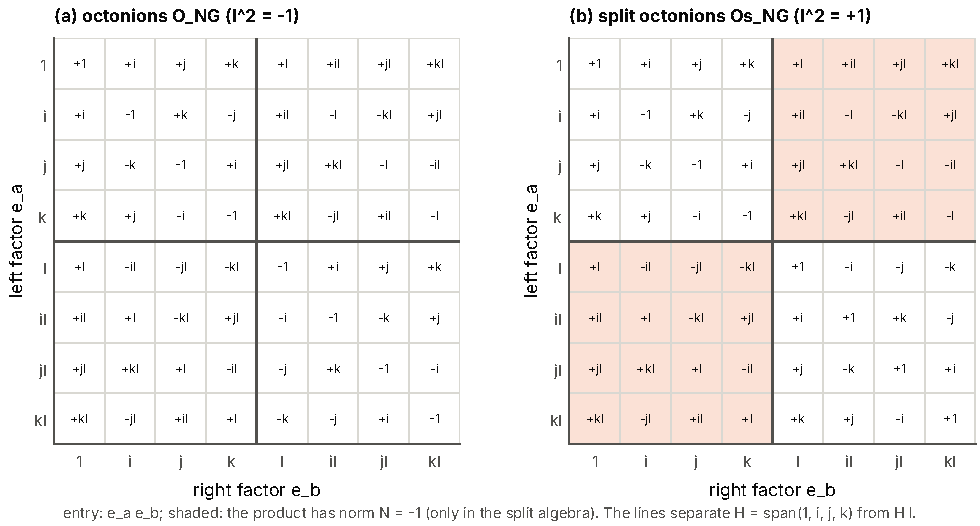
\includegraphics[width=0.92\textwidth]{../figures/fig_ng_tables.pdf}
\caption{Multiplication tables of the octonions (a) and the split octonions (b): the row gives the
left factor, the column the right factor, the entry their product. Shaded: products of norm $-1$
(only in the split algebra). The lines separate the quaternions from their complement. Data:
\texttt{data/ng\_octonion\_tables.csv}.}
\label{fig:tables}
\end{figure*}

The program verifies, in exact integer arithmetic and for both algebras, the following facts
(checks O-1 to O-13 of Appendix~\ref{app:checks}).

\emph{Composition.} $N_{\rm NG}(\mathsf x\mathsf y)=N_{\rm NG}(\mathsf x)N_{\rm NG}(\mathsf y)$. Because both sides
are polynomials of degree four, it suffices to verify the fully polarized identity
$\langle\mathsf x\mathsf y,\mathsf z\mathsf w\rangle_{\rm NG}+\langle\mathsf x\mathsf w,\mathsf z\mathsf y\rangle_{\rm NG}=
2\langle\mathsf x,\mathsf z\rangle_{\rm NG}\langle\mathsf y,\mathsf w\rangle_{\rm NG}$ on all $8^4=4096$ quadruples of
basis elements, which the program does.

\emph{Alternativity and non-associativity.} The associator $(\mathsf x,\mathsf y,\mathsf z)=(\mathsf x\mathsf y)\mathsf z-
\mathsf x(\mathsf y\mathsf z)$ is trilinear, so it is known once it is known on basis elements. It is
totally antisymmetric (the algebras are \emph{alternative}), but it is not zero: it vanishes on
344 of the 512 ordered triples of basis elements and is nonzero on the other
168, which are the triples of three different imaginary units that do not lie in one
quaternionic subalgebra; for example $(\mathsf e_1,\mathsf e_2,\mathsf e_4)=\mathsf e_3\mathsf e_4-\mathsf e_1\mathsf e_6=
\mathsf e_7-(-\mathsf e_7)=2\mathsf e_7$. Alternative algebras obey the Moufang identities
$\mathsf z(\mathsf x(\mathsf z\mathsf y))=((\mathsf z\mathsf x)\mathsf z)\mathsf y$, $\mathsf x(\mathsf z(\mathsf y\mathsf z))=
((\mathsf x\mathsf z)\mathsf y)\mathsf z$ and $(\mathsf z\mathsf x)(\mathsf y\mathsf z)=(\mathsf z(\mathsf x\mathsf y))\mathsf z$; the
program confirms them on 2000 random triples with integer coefficients.

\emph{The commutator algebra is not a Lie algebra.} The commutator $[\mathsf x,\mathsf y]=\mathsf x\mathsf y-
\mathsf y\mathsf x$ of two imaginary elements is imaginary. Its Jacobiator
\begin{equation}
\mathrm{Jac}_{\rm NG}(\mathsf x,\mathsf y,\mathsf z)=[[\mathsf x,\mathsf y],\mathsf z]+[[\mathsf y,\mathsf z],\mathsf x]+[[\mathsf z,\mathsf x],\mathsf y]
\label{eq:jacobiator}
\end{equation}
is, in any algebra, the sum of the six associators of $\mathsf x,\mathsf y,\mathsf z$ taken in all orders
with the signs of the permutations; in an alternative algebra each of them equals $(\mathsf x,\mathsf y,\mathsf z)$
times that sign, so $\mathrm{Jac}_{\rm NG}(\mathsf x,\mathsf y,\mathsf z)=6(\mathsf x,\mathsf y,\mathsf z)$, which the program verifies
on all basis triples. The Jacobiators of the imaginary basis elements span all seven imaginary
directions (rank 7). The imaginary octonions with this commutator form a Malcev
algebra~\cite{Malcev1955} (they satisfy the Malcev identity $\mathrm{Jac}_{\rm NG}(\mathsf x,\mathsf y,[\mathsf x,\mathsf z])=
[\mathrm{Jac}_{\rm NG}(\mathsf x,\mathsf y,\mathsf z),\mathsf x]$, checked), not a Lie algebra.

\emph{Theorem 1 (octonionic charges have no operator representation).} Let $\rho_{\rm NG}$ be a linear
map from the imaginary octonions (or split octonions) to the linear operators on some vector space
with $\rho_{\rm NG}([\mathsf x,\mathsf y])=\rho_{\rm NG}(\mathsf x)\rho_{\rm NG}(\mathsf y)-\rho_{\rm NG}(\mathsf y)
\rho_{\rm NG}(\mathsf x)$. Then $\rho_{\rm NG}=0$.
\emph{Proof.} Products of operators are associative, so the Jacobiator of any three operators
vanishes, and $\rho_{\rm NG}(\mathrm{Jac}_{\rm NG}(\mathsf x,\mathsf y,\mathsf z))=0$. Since the Jacobiators span all imaginary
elements, $\rho_{\rm NG}$ vanishes on all of them. $\square$

Charges that obey the octonionic commutation relations therefore cannot be generators of
symmetries in any quantum theory on a Hilbert space (hypothesis H0): the non-associativity of the
octonions removes them from the reach of the no-go theorems only by removing them from quantum
mechanics. (Octonionic quantum mechanics exists only for the exceptional Jordan algebra of $3\times3$
octonionic Hermitian matrices~\cite{JordanNeumannWigner1934,GunaydinPironRuegg1978}, which has no
tensor products and hence no scattering of several particles.) What survives in quantum mechanics
is the associative envelope: the left multiplications $L_{\rm NG}(\mathsf x)$, $\mathsf y\mapsto\mathsf x\mathsf y$,
are $8\times8$ matrices, and the Lie algebra that the seven $L_{\rm NG}(\mathsf e_1),\dots,
L_{\rm NG}(\mathsf e_7)$ generate under commutators has dimension 28 and is the whole rotation algebra
$\mathfrak{so}(8)$ (octonions) or $\mathfrak{so}(4,4)$ (split octonions) of the norm (check O-12). In the
associative world the octonionic ``charges'' \emph{are} rotation generators of eight dimensions.

\emph{Derivations.} A derivation is a linear map $\mathsf D$ with $\mathsf D(\mathsf x\mathsf y)=(\mathsf D\mathsf x)
\mathsf y+\mathsf x(\mathsf D\mathsf y)$; the derivations generate the automorphisms of the algebra. Solving this
linear condition exactly gives a space of dimension 14 for both algebras, inside the rotations of
the imaginary elements. Its Killing form $B_{\rm NG}(\mathsf D_1,\mathsf D_2)=\mathrm{tr}(\mathrm{ad}\,\mathsf D_1\,
\mathrm{ad}\,\mathsf D_2)$ (with $\mathrm{ad}\,\mathsf D_1$ the matrix of the map $\mathsf D\mapsto[\mathsf D_1,\mathsf D]$ of the derivations into themselves) is negative
definite for $\mathbb O_{\rm NG}$, so its derivations form the compact Lie algebra $\mathfrak g_2$ of the
compact group $\mathrm G_2$, and has $8$ positive and $6$ negative eigenvalues for $\mathbb O'_{\rm NG}$, the split real
form of $\mathfrak g_2$ (checks O-10, O-11).

\subsection{The Dirac matrices of the two spacetimes are octonionic}

\emph{$7{+}1$.} Write a point of the $7{+}1$ spacetime as the octonion
$\mathsf x=x4\,\mathsf e_0+x1\,\mathsf e_1+x2\,\mathsf e_2+x3\,\mathsf e_3+x0\,\mathsf e_4+x5\,\mathsf e_5+x6\,\mathsf e_6+x7\,\mathsf e_7$:
the time is the real part, the three directions of ordinary space are the imaginary quaternions, and
$x0,x5,x6,x7$ are the complement $\mathbb H_{\rm NG}\mathsf e_4$. Denote by $u_{\rm NG}(A)$ the index of the
unit attached to the coordinate $xA$ ($u_{\rm NG}(4)=0$, $u_{\rm NG}(j)=j$, $u_{\rm NG}(0)=4$,
$u_{\rm NG}(t)=t$). The metric $\eta_{1671}=\mathrm{diag}(-1,-1,-1,-1,+1,-1,-1,-1)$ of the $7{+}1$ spacetime is
then the real part of the square: $\eta_{1671}(\mathsf x,\mathsf x)=(x4)^2-\sum_{A\ne4}(xA)^2=\mathrm{Re}(\mathsf x^2)$
(check O-14c). The sixteen-dimensional matrices
\begin{align}
\Gamma^4_{71\rm NG}&=\begin{pmatrix}0&\mathsf 1_8\\ \mathsf 1_8&0\end{pmatrix},\nonumber\\
\Gamma^A_{71\rm NG}&=\begin{pmatrix}-L_{\rm NG}(\mathsf e_{u_{\rm NG}(A)})&0\\0&L_{\rm NG}(\mathsf e_{u_{\rm NG}(A)})\end{pmatrix}
\label{eq:gamma71oct}
\end{align}
($A\neq4$; $\mathsf 1_8$ is the unit matrix) satisfy $\Gamma^A_{71\rm NG}\Gamma^C_{71\rm NG}+
\Gamma^C_{71\rm NG}\Gamma^A_{71\rm NG}=2\eta_{1671}^{AC}\mathsf 1_{16}$: for an imaginary unit $\mathsf e$,
alternativity gives $\mathsf e(\mathsf e\mathsf y)=\mathsf e^2\mathsf y=-\mathsf y$, so $L_{\rm NG}(\mathsf e)^2=-\mathsf 1_8$, and
for two different imaginary units $\mathsf e(\mathsf f\mathsf y)+\mathsf f(\mathsf e\mathsf y)=(\mathsf e\mathsf f+\mathsf f\mathsf e)\mathsf y=0$
(check O-14a).

\emph{$4{+}4$.} Write a point as the split octonion $\mathsf x=\sum_A xA\,\mathsf e_A$. The metric
$\eta_{1644}=\mathrm{diag}(+1,+1,+1,+1,-1,-1,-1,-1)$ is the norm, $\eta_{1644}(\mathsf x,\mathsf x)=N_{\rm NG}(\mathsf x)$
(check O-14d), and the matrices
\begin{equation}
\Gamma^A_{44\rm NG}=\begin{pmatrix}0&L_{\rm NG}(\bar{\mathsf e}_A)\\L_{\rm NG}(\mathsf e_A)&0\end{pmatrix}
\label{eq:gamma44oct}
\end{equation}
satisfy the Clifford relations of $\eta_{1644}$, because $L_{\rm NG}(\bar{\mathsf x})L_{\rm NG}(\mathsf x)=
N_{\rm NG}(\mathsf x)\mathsf 1_8$ in a composition algebra (check O-14b).

\emph{Equivalence with the matrices of the project.} The project's Dirac matrices
$\gamma^A_{1671}$ and $\gamma^A_{1644}$ are built from octonion and split-octonion matrices
$\tau^A_{1671}$ and $\tau^A_{1644}$, $\bar\tau^A_{1644}$ in another basis. Two sets of matrices that
satisfy the same Clifford relations are related by a fixed invertible matrix: with $\gamma^K_{1671}$
the ordered product of the $\gamma^A_{1671}$ over an index set $K$, and $\Gamma^K_{71\rm NG}$ the same
product of the $\Gamma^A_{71\rm NG}$, the matrix
\begin{equation}
\mathcal I_{71\rm NG}=\sum_K\Gamma^K_{71\rm NG}\,\mathsf U_{\rm NG}\,(\gamma^K_{1671})^{-1}
\label{eq:intertwiner}
\end{equation}
(sum over the 256 index sets, $\mathsf U_{\rm NG}$ a fixed matrix with one entry 1 and all others 0) obeys
$\mathcal I_{71\rm NG}\gamma^A_{1671}=\Gamma^A_{71\rm NG}\mathcal I_{71\rm NG}$, because multiplying by
$\Gamma^A_{71\rm NG}$ on the left and by $(\gamma^A_{1671})^{-1}$ on the right only permutes the terms.
The program computes $\mathcal I_{71\rm NG}$ and the corresponding matrix $\mathcal I_{44\rm NG}$ of $4{+}4$ (the same
sum with $\Gamma^K_{44\rm NG}$ and $\gamma^K_{1644}$) in integers, finds them invertible (rank 16), and
finds the 256 products $\gamma^K_{1671}$ (and $\gamma^K_{1644}$) linearly independent, so that the
representation is irreducible and the intertwiner is unique up to a factor (check O-15; the two
matrices are in \texttt{data/ng\_intertwiner\_1671.csv} and \texttt{\_1644.csv}). Every statement about the
$\Gamma^A_{71\rm NG}$ or the $\Gamma^A_{44\rm NG}$ is therefore a statement about the $\gamma^A_{1671}$ or the
$\gamma^A_{1644}$ of the project.

\section{Triality: present for 4+4, absent for 7+1}
\label{sec:triality}

Cartan discovered in 1925 that the rotation group of eight dimensions has a symmetry of order three,
\emph{triality}, that permutes its three inequivalent eight-dimensional representations---the vectors
$V_{\rm NG}$ and the two kinds of half-spinors $S^+_{\rm NG}$ and $S^-_{\rm NG}$---and he proved it by identifying all three
spaces with the octonions~\cite{Cartan1925,Baez2002}. In the language of Lie algebras, triality is an
\emph{outer} automorphism of $\mathfrak{so}(8)$: a map of the algebra onto itself that preserves
commutators but is not a conjugation by a rotation. Whether it survives on a spacetime of signature
$7{+}1$ or $4{+}4$ is a question about the \emph{real form} of the algebra, and the answers differ.

\emph{Local triality.} Let $\mathbb A_{\rm NG}$ be $\mathbb O_{\rm NG}$ or $\mathbb O'_{\rm NG}$ and
$\mathfrak{so}(N_{\rm NG})$ the Lie algebra of the linear maps $\mathsf m$ of the algebra that preserve its
norm infinitesimally, $\langle\mathsf m\mathsf x,\mathsf y\rangle_{\rm NG}+\langle\mathsf x,\mathsf m\mathsf y\rangle_{\rm NG}=0$:
$\mathfrak{so}(8)$ for the octonions, $\mathfrak{so}(4,4)$ for the split octonions. The principle of local
triality~\cite{Schafer1966} states that for every $\mathsf m_1$ in this algebra there is exactly one pair
$(\mathsf m_2,\mathsf m_3)$ in it with
\begin{equation}
\mathsf m_1(\mathsf x\mathsf y)=(\mathsf m_2\mathsf x)\mathsf y+\mathsf x(\mathsf m_3\mathsf y)\qquad\text{for all }\mathsf x,\mathsf y.
\label{eq:lt}
\end{equation}
For each of the 28 basis elements $\mathsf m_1$ the program writes Eq.~(\ref{eq:lt}) on all 64 pairs of
basis elements as 512 linear equations for the 56 coefficients of $\mathsf m_2$ and $\mathsf m_3$ and solves
them exactly: the system is consistent and its solution unique, for both algebras (check T-1). The
maps $T^{(2)}_{\rm NG}:\mathsf m_1\mapsto\mathsf m_2$ and $T^{(3)}_{\rm NG}:\mathsf m_1\mapsto\mathsf m_3$ preserve all
378 commutators of basis elements, are invertible, and are involutions (checks T-2, T-3).

\emph{They are outer.} A conjugation by a matrix does not change the characteristic polynomial. The
generator $\mathsf r_{01}$ of rotations in the plane of $\mathsf e_0$ and $\mathsf e_1$ (with
$\mathsf r_{01}\mathsf e_1=\mathsf e_0$, $\mathsf r_{01}\mathsf e_0=-\mathsf e_1$, and zero on the other six units) has
$\det(\lambda_{\rm NG}\mathsf 1_8-\mathsf r_{01})=\lambda_{\rm NG}^6(\lambda_{\rm NG}^2+1)$, the spectrum of a vector
representation (eigenvalues $\pm i$ and six zeros). Its images have
$\det(\lambda_{\rm NG}\mathsf 1_8-T^{(2)}_{\rm NG}\mathsf r_{01})=\det(\lambda_{\rm NG}\mathsf 1_8-T^{(3)}_{\rm NG}\mathsf r_{01})=
(\lambda_{\rm NG}^2+\tfrac14)^4$, the spectrum of a half-spinor representation (eigenvalues $\pm i/2$, four
times each), computed exactly (check T-4, Fig.~\ref{fig:triality}). With the conjugation
$\kappa_{\rm NG}:\mathsf x\mapsto\bar{\mathsf x}$, which is a reflection and induces the automorphism
$\mathrm{Ad}\,\kappa_{\rm NG}:\mathsf m\mapsto\kappa_{\rm NG}\mathsf m\kappa_{\rm NG}$, the composition
$\vartheta_{\rm NG}=T^{(2)}_{\rm NG}\circ\mathrm{Ad}\,\kappa_{\rm NG}$ has order three ($\vartheta_{\rm NG}^3=1\ne
\vartheta_{\rm NG}$), and $\mathrm{Ad}\,\kappa_{\rm NG}\,\vartheta_{\rm NG}\,\mathrm{Ad}\,\kappa_{\rm NG}=
\vartheta_{\rm NG}^{-1}$: these automorphisms generate the permutation group of three objects, the outer
automorphism group of $\mathfrak{so}(8)$ (check T-5). For the split octonions the program also confirms
that the images have exactly the spectrum of the half-spinor generators of the project: the two
$8\times8$ diagonal blocks of $\Sigma^{01}_{1644}=\tfrac14[\gamma^0_{1644},\gamma^1_{1644}]$, which act on
the real half-spinors $S^\pm_{\rm NG}$ of $4{+}4$, both have the characteristic polynomial
$(\lambda_{\rm NG}^2+\tfrac14)^4$ (check T-6).

\begin{figure}[t]
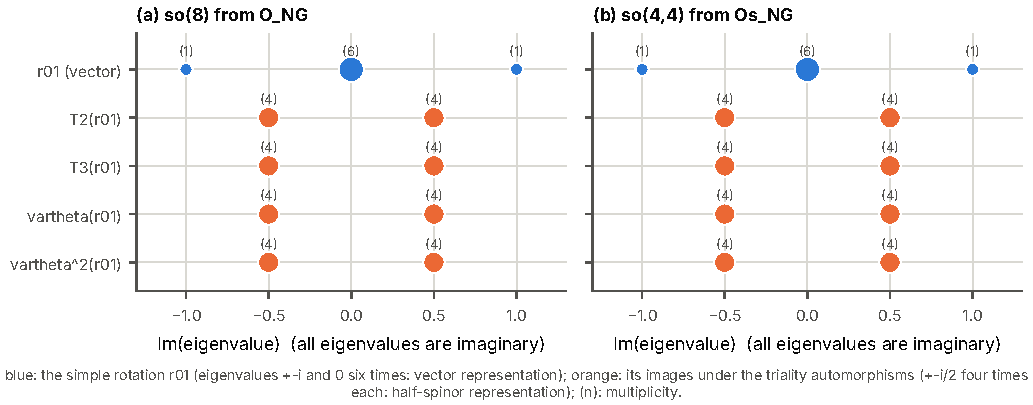
\includegraphics[width=\columnwidth]{../figures/fig_ng_triality.pdf}
\caption{Triality changes the spectrum of a rotation generator from that of a vector (blue: $\pm i$
and six zeros) to that of a half-spinor (orange: $\pm i/2$, four times each), for $\mathfrak{so}(8)$ (a)
and $\mathfrak{so}(4,4)$ (b). The numbers give multiplicities. Data:
\texttt{data/ng\_triality\_charpolys.csv} (exact characteristic polynomials).}
\label{fig:triality}
\end{figure}

\emph{Theorem 2 (no triality for $7{+}1$).} No automorphism of the Lorentz algebra
$\mathfrak{so}(7,1)$ maps its vector representation onto a half-spinor representation.
\emph{Proof.} (a) A real representation whose commuting matrices (its \emph{commutant}) form the
real numbers is of real type; one whose commutant is a copy of the complex numbers is of complex
type. Composing a representation with an automorphism does not change its matrices as a set, hence
not its commutant or its type. (b) The vector representation of $\mathfrak{so}(7,1)$ has commutant
$\mathbb R$ (check T-7d). (c) On the 16 real spinor components the commutant of the 28 generators
$\Sigma^{AB}_{1671}$ is spanned by $\mathsf 1_{16}$ and $\omega_{1671}=\gamma^0_{1671}\cdots
\gamma^7_{1671}$, and $\omega_{1671}^2=-\mathsf 1_{16}$ (check T-7b): the spinor representation is
irreducible over the real numbers and of complex type, so there is no real half-spinor representation
of dimension 8 at all; over the complex numbers the two half-spinors are complex conjugates of each
other. Hence no automorphism can map the vector representation (real type, dimension 8) onto a
half-spinor. $\square$

By contrast, on $4{+}4$ the commutant of the $\Sigma^{AB}_{1644}$ is spanned by $\mathsf 1_{16}$ and
$\omega_{1644}$ with $\omega_{1644}^2=+\mathsf 1_{16}$ (check T-7c): the spinors split into two real
half-spinors of dimension 8 (Majorana-Weyl spinors), and triality permutes $V_{\rm NG}$, $S^+_{\rm NG}$, $S^-_{\rm NG}$, all real.
A direct test agrees: for the boost $\mathsf m_1$ that mixes $\mathsf e_0$ with $\mathsf e_1$ in the metric
$\mathrm{Re}(\mathsf x^2)$ of $7{+}1$ (it maps $\mathsf e_0\mapsto\mathsf e_1$ and $\mathsf e_1\mapsto\mathsf e_0$),
Eq.~(\ref{eq:lt}) has no solution even with arbitrary $8\times8$ matrices $\mathsf m_2$, $\mathsf m_3$ (check
T-7a). Cartan's triality lives on the complex algebra $\mathfrak{so}(8,\mathbb C)$ and on those of its real
forms whose three eight-dimensional representations are real---the compact $\mathfrak{so}(8)$ and the split
$\mathfrak{so}(4,4)$; the octonions build the Dirac matrices of $7{+}1$ (Sec.~\ref{sec:octonions}), but
the order-three automorphism does not restrict to $\mathfrak{so}(7,1)$, which keeps only the reflection.

\section{Combined Lorentz-internal manifolds}
\label{sec:combined}

\subsection{Definition}

Split the eight coordinates of either spacetime into the four of a four-dimensional world,
$x1,x2,x3$ (space) and $x4$ (time), and the four of a fibre, $x0,x5,x6,x7$. The \emph{combined
manifold} is the product $\mathcal M^{3,1}_{\rm NG}\times\mathcal K_{\rm NG}$ of the four-dimensional
Minkowski spacetime $\mathcal M^{3,1}_{\rm NG}$ (coordinates $x1,\dots,x4$) and the fibre
$\mathcal K_{\rm NG}$ (coordinates $x0,x5,x6,x7$), with the metric $\eta_{1671}$ or $\eta_{1644}$
restricted to each factor: on $7{+}1$ the fibre $\mathcal K^4_{\rm NG}$ is Euclidean, on $4{+}4$ the fibre
$\mathcal K^{1,3}_{\rm NG}$ has one direction ($x0$) with $\eta_{1644}=+1$ and three ($x5,x6,x7$) with
$\eta_{1644}=-1$. Its tangent space at every point is the same eight-dimensional vector space as
before, but its symmetry is reduced from the eight-dimensional Lorentz group to the product of the
Lorentz group of $\mathcal M^{3,1}_{\rm NG}$ and the rotation group of $\mathcal K_{\rm NG}$. We consider two
readings of the fibre, which Sec.~\ref{sec:renorm} distinguishes sharply: (i) \emph{geometric}: a
compact manifold, for example a torus of radius $R_{\rm NG}$, on which fields may depend (Kaluza and
Klein~\cite{Kaluza1921,Klein1926}); (ii) \emph{internal}: the fields do not depend on $x0,x5,x6,x7$, so the
fibre carries no momentum and its rotations act on the field components only, like an internal
symmetry. Figure~\ref{fig:manifolds} shows the split and its octonionic meaning: on $7{+}1$ the
four-dimensional world is the algebra of quaternions inside the octonions (time is the real unit) and
the fibre is its complement $\mathbb H_{\rm NG}\mathsf e_4$; on $4{+}4$ the world is spanned by
$\mathsf e_1,\mathsf e_2,\mathsf e_3,\mathsf e_4$ and the fibre by $\mathsf e_0,\mathsf e_5,\mathsf e_6,\mathsf e_7$.

\begin{figure}[t]
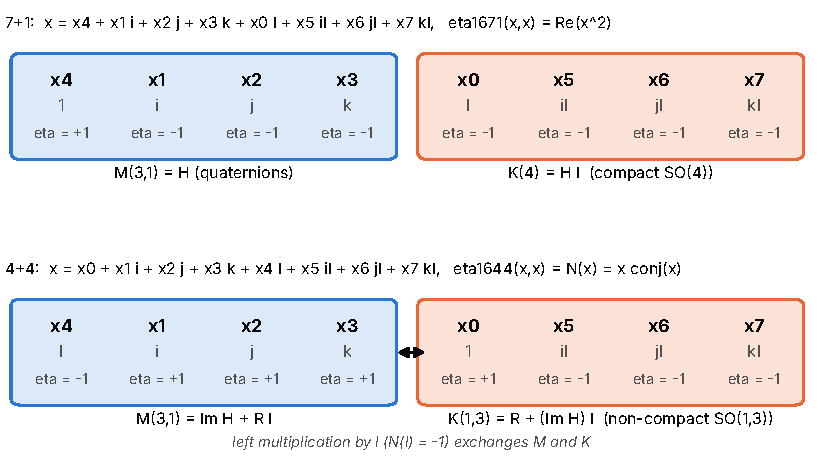
\includegraphics[width=\columnwidth]{../figures/fig_ng_manifolds.pdf}
\caption{The two combined manifolds: the coordinates, the octonion units attached to them, and the
signs of the metric. Blue: the four-dimensional world $\mathcal M^{3,1}_{\rm NG}$; orange: the fibre
$\mathcal K_{\rm NG}$. On $4{+}4$ the left multiplication by $\mathsf e_4$ (norm $-1$) exchanges the two.}
\label{fig:manifolds}
\end{figure}

\subsection{Lorentz generators become internal generators}

The 28 generators $\Sigma^{AB}_{1671}=\tfrac14[\gamma^A_{1671},\gamma^B_{1671}]$ of the eight-dimensional
Lorentz algebra fall into three sets: the six with $A,B$ both in $\{1,2,3,4\}$ (the Lorentz algebra
$\mathfrak{so}(3,1)$ of the world), the six with $A,B$ both in $\{0,5,6,7\}$ (the rotations of the fibre),
and the 16 mixed ones. The first two sets commute exactly, and every mixed generator fails to commute
with some generator of the first set (check K-1); the same holds for $4{+}4$. On the combined manifold
only the first two sets remain symmetries, and the second set acts on the fields \emph{at each point of
the world}: from the four-dimensional point of view it is an internal symmetry, although it is a
part of the eight-dimensional Lorentz group. This is the precise sense in which Lorentz degrees of
freedom become internal ones; the conclusion of the Coleman-Mandula theorem holds in four
dimensions (the world's Lorentz algebra and the fibre algebra commute), and in eight dimensions its
hypothesis H1 fails, because the background---the product structure---is not invariant under the
mixed generators.

\emph{Compact on $7{+}1$, non-compact on $4{+}4$.} On $7{+}1$ every generator $2\Sigma^{ab}_{1671}=
\gamma^a_{1671}\gamma^b_{1671}$ of the fibre squares to $-\mathsf 1_{16}$, so its eigenvalues are imaginary;
the trace form of the six generators (the trace of the product of two of them, as a quadratic form on their real combinations) is negative definite, and the fibre
algebra is the compact $\mathfrak{so}(4)$. On $4{+}4$ the three generators $2\Sigma^{0t}_{1644}$ square to
$+\mathsf 1_{16}$ and the trace form has signature $(3,3)$: the fibre algebra is the non-compact
$\mathfrak{so}(1,3)$ (check K-2). \emph{Theorem 3.} No positive-definite scalar product on the 16
components is invariant under the fibre algebra of $4{+}4$. \emph{Proof.} If a positive-definite scalar
product were invariant, every generator would be anti-Hermitian with respect to it and would have
purely imaginary eigenvalues; $\Sigma^{05}_{1644}$ has the real eigenvalues $\pm\tfrac12$. $\square$
The eight-dimensionally covariant density shows the same: on $7{+}1$ the Dirac conjugation matrix
$\mathsf A_{\rm NG}=\gamma^4_{1671}$, defined by $\mathsf A_{\rm NG}\Sigma^{AB}_{1671}\mathsf A_{\rm NG}^{-1}=
-(\Sigma^{AB}_{1671})^\dagger$ for all 28 generators, gives the density $\psi^\dagger_{1671}\mathsf A_{\rm NG}
\gamma^4_{1671}\psi_{1671}=\psi^\dagger_{1671}\psi_{1671}$, positive; on $4{+}4$ the conjugation matrix is
$\mathsf A_{\rm NG}=\gamma^4_{1644}\gamma^5_{1644}\gamma^6_{1644}\gamma^7_{1644}$ and the density matrix
$\mathsf A_{\rm NG}\gamma^4_{1644}=\gamma^5_{1644}\gamma^6_{1644}\gamma^7_{1644}$ is traceless with square
$\mathsf 1_{16}$, so the density is indefinite and the Fock space has states of negative norm (check K-7).
A theory of the $4{+}4$ field with positive norm keeps, of the fibre algebra, only its compact form,
spanned by $\Sigma^{st}_{1644}$ and $i\Sigma^{0t}_{1644}$ (Sec.~\ref{sec:superfluid}).

\emph{Spinors.} In statements that hold on both spacetimes, $\gamma^A_{\rm NG}$ denotes the Dirac
matrices of the spacetime under discussion ($\gamma^A_{1671}$ or $\gamma^A_{1644}$), and likewise
$\Sigma^{AB}_{\rm NG}$, $\omega_{\rm NG}$, $C^\pm_{\rm NG}$, $\beta_{\rm NG}$, $\alpha^j_{\rm NG}$ (the matrices
of the project), $\psi_{\rm NG}$ (the field $\psi_{1671}$ or $\psi_{1644}$) and $m_{\rm NG}$ (its mass). The products
$\omega^{\rm 4D}_{\rm NG}=\gamma^1_{\rm NG}\gamma^2_{\rm NG}\gamma^3_{\rm NG}\gamma^4_{\rm NG}$ and
$\omega^{\rm int}_{\rm NG}=\gamma^0_{\rm NG}\gamma^5_{\rm NG}\gamma^6_{\rm NG}\gamma^7_{\rm NG}$ commute; the 16
products of $\gamma^1_{\rm NG},\dots,\gamma^4_{\rm NG}$ and the 16 products of
$\omega^{\rm 4D}_{\rm NG}\gamma^a_{\rm NG}$ are each linearly independent, and the two sets commute, so the 16 components are the tensor product of a
four-dimensional Dirac spinor of the world and a four-component spinor of the fibre (check K-3). On
$7{+}1$, $(\omega^{\rm int}_{\rm NG})^2=+\mathsf 1_{16}$ splits the fibre spinor into the two real doublets of
$\mathfrak{so}(4)=\mathfrak{su}(2)\oplus\mathfrak{su}(2)$; on $4{+}4$, $(\omega^{\rm int}_{\rm NG})^2=-\mathsf 1_{16}$ and the
two doublets are complex conjugates, as for the Lorentz group.

\subsection{The octonions lock rotations to internal rotations}

The octonions carry the \emph{associative three-form} $\phi_{\rm NG}(\mathsf x,\mathsf y,\mathsf z)=
\langle\mathsf x,\mathsf y\mathsf z\rangle_{\rm NG}$ on the imaginary units; its symmetry group in the rotations
of the seven imaginary directions is $\mathrm G_2$. Consider, on $7{+}1$, the rotations of ordinary space
(the imaginary quaternions $\mathsf e_1,\mathsf e_2,\mathsf e_3$, algebra $\mathfrak{so}(3)$) and of the fibre
($\mathsf e_4,\dots,\mathsf e_7$, algebra $\mathfrak{so}(4)$). Inside $\mathfrak{so}(3)\oplus\mathfrak{so}(4)$ (dimension 9)
the elements that leave $\phi_{\rm NG}$ unchanged form an algebra of dimension
6; the same algebra leaves unchanged the six components
$\phi_{\rm NG}(\mathsf e_j,\mathsf e_{u_{\rm NG}(a)},\mathsf e_{u_{\rm NG}(b)})$ with one unit of ordinary space and two of the fibre (their part
$\phi^{\rm mix}_{\rm NG}$). It projects \emph{onto} the space rotations (rank
3), contains no rotation of space alone (dimension 0), and
contains 3 rotations of the fibre alone (checks K-5a, K-5b; Fig.~\ref{fig:locking}).
The same six-dimensional algebra is obtained from the derivations: the elements of
$\mathrm{Der}(\mathbb O_{\rm NG})=\mathfrak g_2$ that preserve the quaternions and their complement (check
K-5c). \emph{Every rotation of space that preserves the octonionic structure is accompanied by a
rotation of the fibre.}

\begin{figure}[t]
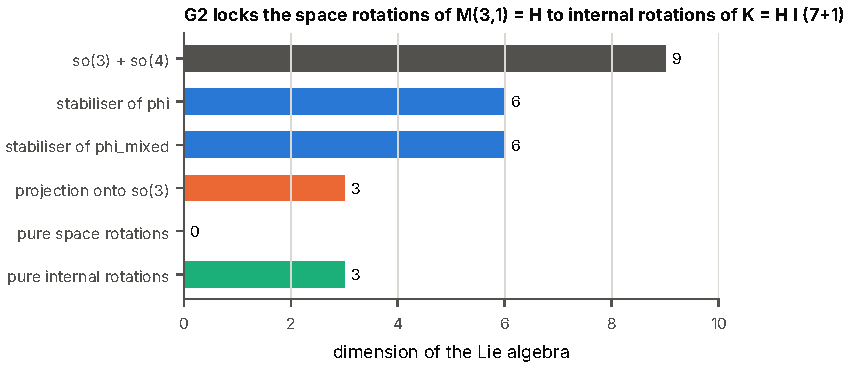
\includegraphics[width=\columnwidth]{../figures/fig_ng_locking.pdf}
\caption{Dimensions of the Lie algebras of the $\mathrm G_2$ locking on $7{+}1$. Of the nine rotations of
space and fibre, six preserve the associative three-form; they include every rotation of space, but
none without a rotation of the fibre. Data: \texttt{data/ng\_g2\_locking.csv}.}
\label{fig:locking}
\end{figure}

A background with these symmetries is a condensate of the pairs $\psi^T_{1671}C^+_{1671}
\gamma^j_{1671}\gamma^a_{1671}\gamma^b_{1671}\psi_{1671}$, with one space index and two fibre indices, whose
amplitudes are proportional to $\phi_{\rm NG}(\mathsf e_j,\mathsf e_{u_{\rm NG}(a)},\mathsf e_{u_{\rm NG}(b)})$. These
pairs are nonzero but vanish for two particles at rest (they are p-wave pairs, Sec.~\ref{sec:superfluid}),
and the condensate picks a rest frame: it can exist only in a medium, which breaks the boosts
(hypothesis H1). In such a medium the unbroken rotations are the diagonal combinations of space and
fibre rotations---the octonionic analogue of the B phase of superfluid helium-3, where the
condensate locks spin to orbital rotations~\cite{BalianWerthamer1963,Leggett1975}, of the
colour-flavour locking of dense quark matter~\cite{AlfordRajagopalWilczek1999}, and of the
``spin from isospin'' of Refs.~\cite{JackiwRebbi1976,HasenfratzTHooft1976}.

\subsection{Split octonions exchange space-time and fibre}

On $4{+}4$ the left multiplication $L_{\rm NG}(\mathsf e_4)$ by the split unit $\mathsf e_4$, of norm $-1$, is an
\emph{anti-isometry}: $N_{\rm NG}(\mathsf e_4\mathsf x)=-N_{\rm NG}(\mathsf x)$, and $L_{\rm NG}(\mathsf e_4)^2=\mathsf 1_8$.
It maps $\mathsf e_1,\mathsf e_2,\mathsf e_3,\mathsf e_4$ (the world) onto $\pm\mathsf e_5,\pm\mathsf e_6,\pm\mathsf e_7,
\mathsf e_0$ (the fibre) and back, and conjugation by it maps the Lorentz algebra $\mathfrak{so}(3,1)$ of the
world onto the algebra $\mathfrak{so}(1,3)$ of the fibre and back (check K-6). Since the overall sign of
a metric is a convention, the split-octonion product makes the distinction between space-time and
internal directions of $4{+}4$ a matter of choice; together with triality (Sec.~\ref{sec:triality}),
which permutes vectors and spinors, even the distinction between space-time vectors and spinors is
not invariant. On $7{+}1$ no such exchange exists: the Lorentz algebra of the world, with trace form of
signature $(3,3)$, is not isomorphic to the compact fibre algebra (check K-2).

\subsection{Mass splitting and the Kaluza-Klein spectrum}

\emph{O'Raifeartaigh.} A rotation of $7{+}1$ in the plane of $x1$ and $x0$ with cosine $\tfrac35$ and
sine $\tfrac45$ is an element of the eight-dimensional Poincar\'e group, which is finite-dimensional
and contains the four-dimensional one. Applied to a momentum with time component 5 and $x1$
component 3, it keeps the eight-dimensional mass squared 16 but changes the four-dimensional mass
squared $(5)^2-(\text{space part})^2$ from 16 to $\tfrac{544}{25}$ (exact, check K-8). There is no
contradiction with the theorem: a single eight-dimensional particle has a continuous spectrum of
four-dimensional masses, from its eight-dimensional mass upwards, so hypothesis H7 fails.

\emph{Kaluza-Klein modes.} On a torus fibre of radius $R_{\rm NG}$ a field of mass $m_{\rm NG}$ (the
mass $m_{1671}$ or $m_{1644}$ of the field of the spacetime under discussion) has the modes
$\exp(i\sum_a n^a_{\rm NG}x^a/R_{\rm NG})$ with integers $n^a_{\rm NG}$. Squaring the Dirac equation
$(i\gamma^A_{1671}\partial_A-m_{1671})\psi_{1671}=0$ of $7{+}1$ gives $(\eta^{AB}_{1671}\partial_A\partial_B+
m_{1671}^2)\psi_{1671}=0$, and squaring the Dirac equation $(\gamma^A_{1644}\partial_A-m_{1644})\psi_{1644}=0$
of $4{+}4$ gives $(\eta^{AB}_{1644}\partial_A\partial_B-m_{1644}^2)\psi_{1644}=0$. Inserting a mode with energy
$\varepsilon_{\rm NG}$ and momentum $\vec q$ in the world gives $\varepsilon_{\rm NG}^2=q^2+(m^{\rm eff}_{\rm NG})^2$ with
the four-dimensional mass squared
\begin{align}
(m^{\rm eff}_{\rm NG})^2&=m_{1671}^2+\textstyle\sum_a(n^a_{\rm NG})^2/R_{\rm NG}^2\quad(7{+}1),\nonumber\\
(m^{\rm eff}_{\rm NG})^2&=m_{1644}^2+\big[(n^0_{\rm NG})^2-\textstyle\sum_t(n^t_{\rm NG})^2\big]/R_{\rm NG}^2\quad(4{+}4).
\label{eq:kkmass}
\end{align}
On $7{+}1$ it is never negative; on $4{+}4$ it is negative for most modes: a tower of tachyons. With $(m_{\rm NG}R_{\rm NG})^2=1$
and $\lvert n^a_{\rm NG}\rvert\le n^{\max}_{\rm NG}=12$ the tachyonic fraction is 0.8660 (check K-9,
Fig.~\ref{fig:kk}). A geometric $4{+}4$ fibre is therefore inconsistent: the $4{+}4$ combined manifold
admits only the internal reading, in which the fibre carries no momentum.

\begin{figure*}[t]
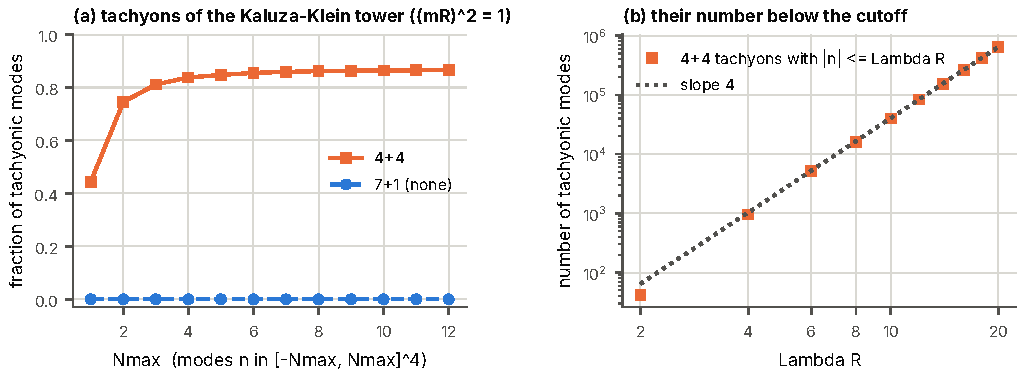
\includegraphics[width=0.92\textwidth]{../figures/fig_ng_kk.pdf}
\caption{Kaluza-Klein modes on a torus fibre with $(m_{\rm NG}R_{\rm NG})^2=1$. (a) Fraction of tachyonic
modes among all modes with $\lvert n^a_{\rm NG}\rvert\le n^{\max}_{\rm NG}$ (Nmax in the figure): none on $7{+}1$,
most of them on $4{+}4$.
(b) The number of $4{+}4$ tachyons with $\sum_a(n^a_{\rm NG})^2\le(\Lambda_{\rm NG}R_{\rm NG})^2$ grows like
$(\Lambda_{\rm NG}R_{\rm NG})^4$. Data: \texttt{data/ng\_kk\_tachyons.csv},
\texttt{data/ng\_kk\_tachyons\_cutoff.csv}.}
\label{fig:kk}
\end{figure*}

\section{The graded loophole: supersymmetry in eight dimensions}
\label{sec:susy}

\subsection{The super-Poincar\'e algebras}

The one extension of the conclusion of Coleman and Mandula that survives all their hypotheses is a
superalgebra~\cite{HLS1975,Nahm1978,Strathdee1987}. We build it explicitly on both spacetimes, with
the matrices of the project. Its generators are the 28 Lorentz generators $\mathcal J^{AB}_{\rm NG}$
($A<B$), the 8 momenta $\mathcal P^{\rm NG}_C$, 16 supercharges $\mathcal Q^{\rm NG}_l$ ($l=1,\dots,16$, one
for each real spinor component), and an R-charge $\mathcal R_{\rm NG}$. With the metric
$\eta_{\rm NG}$ of the spacetime (diagonal, entries $\eta_{AA}^{\rm NG}=\pm1$), the nonzero brackets are
\begin{subequations}
\label{eq:superalgebra}
\begin{align}
[\mathcal J^{AB}_{\rm NG},\mathcal J^{CD}_{\rm NG}]&=\eta^{\rm NG}_{BC}\mathcal J^{AD}_{\rm NG}-\eta^{\rm NG}_{AC}\mathcal J^{BD}_{\rm NG}\nonumber\\
&\quad-\eta^{\rm NG}_{BD}\mathcal J^{AC}_{\rm NG}+\eta^{\rm NG}_{AD}\mathcal J^{BC}_{\rm NG},\\
[\mathcal J^{AB}_{\rm NG},\mathcal P^{\rm NG}_C]&=\eta^{\rm NG}_{BC}\mathcal P^{\rm NG}_A-\eta^{\rm NG}_{AC}\mathcal P^{\rm NG}_B,\\
[\mathcal J^{AB}_{\rm NG},\mathcal Q^{\rm NG}_l]&=\sum_{l'}(\Sigma^{\rm NG}_{AB})_{l'l}\,\mathcal Q^{\rm NG}_{l'},\\
\{\mathcal Q^{\rm NG}_l,\mathcal Q^{\rm NG}_{l'}\}&=\sum_C(\mathsf Y^C_{\rm NG})_{ll'}\,\mathcal P^{\rm NG}_C,\\
[\mathcal R_{\rm NG},\mathcal Q^{\rm NG}_l]&=\sum_{l'}(\omega_{\rm NG})_{l'l}\,\mathcal Q^{\rm NG}_{l'},
\end{align}
\end{subequations}
where $\mathcal J^{BA}_{\rm NG}=-\mathcal J^{AB}_{\rm NG}$ and $\mathcal J^{AA}_{\rm NG}=0$, the spinor generators
with lowered indices are $\Sigma^{\rm NG}_{AB}=\eta^{\rm NG}_{AA}\eta^{\rm NG}_{BB}\Sigma^{AB}_{\rm NG}$, and the
matrices of the anticommutator are $\mathsf Y^C_{\rm NG}=2C^+_{\rm NG}\gamma^C_{\rm NG}$. On both spacetimes
$C^+_{\rm NG}\gamma^C_{\rm NG}(C^+_{\rm NG})^{-1}=(\gamma^C_{\rm NG})^T$ and $C^+_{\rm NG}$ is symmetric, so every
$\mathsf Y^C_{\rm NG}$ is symmetric, as an anticommutator requires; the R-charge acts through
$\omega_{\rm NG}=\gamma^0_{\rm NG}\cdots\gamma^7_{\rm NG}$, which commutes with every
$\gamma^A_{\rm NG}\gamma^B_{\rm NG}$, so $\mathcal R_{\rm NG}$ commutes with $\mathcal J^{AB}_{\rm NG}$ and
$\mathcal P^{\rm NG}_C$: it is an internal symmetry. It does not commute with the supercharges, and their
anticommutator is a momentum. Lorentz and internal symmetry are tied together through the odd
generators.

The program builds the complete table of brackets of the 53 generators and checks the graded Jacobi
identity, $(-1)^{|\mathsf x||\mathsf z|}[\mathsf x,[\mathsf y,\mathsf z]\}+\text{cyclic}=0$ with $|\mathsf x|=1$ for a
supercharge and 0 otherwise, on every one of the 148877 ordered triples of generators,
on both spacetimes: no triple violates it (checks S-1, S-2a). All structure constants are integers,
halves or quarters; binary floating-point arithmetic represents them and all their sums and
products exactly, so the check is exact.

\subsection{Positivity: present on 7+1, absent on 4+4}

For Hermitian supercharges the matrix $\{\mathcal Q^{\rm NG}_l,\mathcal Q^{\rm NG}_{l'}\}$ has a nonnegative
expectation value in every state, because $\langle\{\mathcal Q^{\rm NG}_{\mathsf v},\mathcal Q^{\rm NG}_{\mathsf v}\}\rangle=
2\lVert\mathcal Q^{\rm NG}_{\mathsf v}\lvert\cdot\rangle\rVert^2$ for every real combination $\mathcal Q^{\rm NG}_{\mathsf v}=\sum_l\mathsf v^l\mathcal Q^{\rm NG}_l$ of them (with real coefficients $\mathsf v^l$ and any state $\lvert\cdot\rangle$).
On $7{+}1$, $C^+_{1671}\gamma^4_{1671}=\mathsf 1_{16}$, and the seven matrices $C^+_{1671}\gamma^A_{1671}$ with
$A\neq4$ anticommute and square to $\mathsf 1_{16}$ (check S-4). Hence
$\sum_C\mathsf Y^C_{\rm NG}\mathcal P^{\rm NG}_C$ has the eigenvalues
$2(\mathcal P^{\rm NG}_4\pm\lvert\vec{\mathcal P}_{\rm NG}\rvert)$, with $\lvert\vec{\mathcal P}_{\rm NG}\rvert^2=
\sum_{A\neq4}(\mathcal P^{\rm NG}_A)^2$: it is positive exactly for momenta in the forward light cone, and
unitary representations of positive energy exist. The R-symmetry is compact: $\omega_{1671}^2=
-\mathsf 1_{16}$, so $\exp(\varphi_{\rm NG}\omega_{1671})=\cos\varphi_{\rm NG}+\omega_{1671}\sin\varphi_{\rm NG}$ is a rotation by an
angle $\varphi_{\rm NG}$, a group $U(1)$. This is the minimal supersymmetry algebra of eight dimensions, with 16 real
supercharges~\cite{Strathdee1987,KugoTownsend1983}.

On $4{+}4$ every $\mathsf Y^C_{\rm NG}=2C^+_{1644}\gamma^C_{1644}$ is traceless (a product of an odd number of
different Dirac matrices), so $\sum_C\mathsf Y^C_{\rm NG}\mathcal P^{\rm NG}_C$ is traceless and nonzero for
every nonzero momentum and has a negative eigenvalue (check S-4, Fig.~\ref{fig:susy}): the algebra
exists, its Jacobi identities hold, but it has no unitary representation with nonzero momentum
(hypothesis H8 fails). Its R-symmetry is non-compact, $\omega_{1644}^2=+\mathsf 1_{16}$, and
$\exp(\varphi_{\rm NG}\omega_{1644})$ multiplies the two chiral halves of the supercharges by $\exp(\mp\varphi_{\rm NG})$; since
$\omega_{1644}$ anticommutes with every $\mathsf Y^C_{\rm NG}$, the anticommutator pairs a supercharge of one
chirality with one of the other.

\begin{figure*}[t]
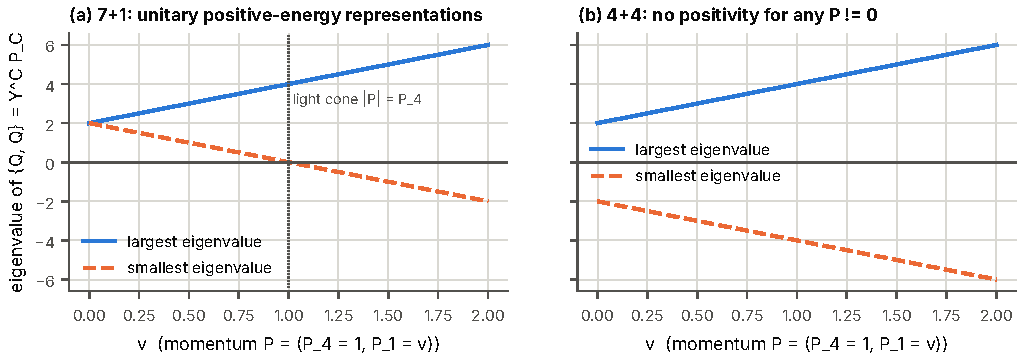
\includegraphics[width=0.92\textwidth]{../figures/fig_ng_superalgebra.pdf}
\caption{Smallest and largest eigenvalue of the matrix $\sum_C\mathsf Y^C_{\rm NG}\mathcal P^{\rm NG}_C$ of the anticommutators $\{\mathcal Q^{\rm NG}_l,\mathcal Q^{\rm NG}_{l'}\}$
for the momentum with $\mathcal P^{\rm NG}_4=1$ and $\mathcal P^{\rm NG}_1=v_{\rm NG}$, all other components zero.
(a) $7{+}1$: both are positive inside the light cone $v_{\rm NG}<1$. (b) $4{+}4$: the smallest is negative for
every momentum. Data: \texttt{data/ng\_superalgebra\_positivity.csv}.}
\label{fig:susy}
\end{figure*}

\subsection{Tensorial charges: a McGlinn-type counterexample}

On $7{+}1$ the matrix $C^+_{1671}\gamma^K_{1671}$ is symmetric exactly when the number $r$ of indices in
$K$ is 0, 1, 4, 5 or 8, because transposition reverses the order of the factors; their numbers
$1+8+70+56+1=136$ add up to the dimension of the space of symmetric $16\times16$ matrices. The most
general anticommutator therefore is
\begin{align}
\{\mathcal Q^{\rm NG}_l,\mathcal Q^{\rm NG}_{l'}\}&=\sum_C(\mathsf Y^C_{\rm NG})_{ll'}\mathcal P^{\rm NG}_C\nonumber\\
&\quad+\sum_{K:\,r\in\{0,4,5,8\}}(C^+_{1671}\gamma^K_{1671})_{ll'}\,\mathcal Z^K_{\rm NG},
\label{eq:tensorial}
\end{align}
with 128 \emph{tensorial charges} $\mathcal Z^K_{\rm NG}$ that commute with the momenta and the
supercharges, and on which the Lorentz generators and the R-charge act as the graded Jacobi identity
dictates (the program determines these actions from it). The extended algebra of 181 generators
satisfies the graded Jacobi identity on all 5929741 triples (check S-2b). Of the
charges, the 126 with four or five indices commute with all momenta but are \emph{not} Lorentz
scalars, and 72 (those with 0, 4 or 8 indices) carry R-charge (check S-3). Generators that commute
with the translations but not with the Lorentz group are what McGlinn's theorem excludes when they
form a semisimple algebra; these form an abelian algebra, so its hypothesis H6 fails. In a theory of
particles alone such charges must vanish~\cite{HLS1975}; they are carried by extended objects.

\section{Where the hypotheses fail in eight dimensions: the counterexamples}
\label{sec:catalogue}

Table~\ref{tab:catalogue} collects the constructions of Secs.~\ref{sec:octonions} to \ref{sec:susy}
and of the superfluid of Sec.~\ref{sec:superfluid}. Each one combines Lorentz and internal symmetry
in a way that the conclusion of the no-go theorems forbids, and each one violates at least one
hypothesis of Table~\ref{tab:hypotheses}; the last column names the machine checks that establish it.
None is a counterexample to a theorem whose hypotheses hold---there is none---but together they map
out how much room eight dimensions, and the octonions in particular, leave.

Three lessons stand out. First, the specifically octonionic mechanisms act on the \emph{first}
hypothesis, H0: non-associativity removes octonionic charges from operator algebras altogether
(Theorem~1), and triality, an automorphism of the Lie algebra rather than an operator, exists only
for the split signature $4{+}4$, which violates H0 (indefinite metric) and H1 (four times) anyway.
Second, on $7{+}1$ the hypotheses H0 and H2 to H5 hold for any reasonable field theory with a mass gap,
and the theorem of Pelc and Horwitz applies: every combination of Lorentz and internal symmetry on
$7{+}1$ requires either odd generators (supersymmetry) or a background that breaks the eight-dimensional
Poincar\'e group (a combined manifold, a medium, a condensate). Third, the combined manifolds turn a
part of the eight-dimensional Lorentz group into an internal group of the four-dimensional world; that
internal group can then be combined freely with other internal symmetries, and the superfluid of
Sec.~\ref{sec:superfluid} does so: its chiral phase leaves unbroken a sum of an eight-dimensional
Lorentz rotation and the fermion number, in a vacuum that is invariant under the four-dimensional
Lorentz group.

\begin{table*}[t]
\caption{The constructions of this paper that combine Lorentz and internal symmetry, the hypothesis
of Table~\ref{tab:hypotheses} that each violates, and the checks of Appendix~\ref{app:checks} that
establish it.}
\label{tab:catalogue}
\begin{ruledtabular}
\begin{tabular}{>{\raggedright\arraybackslash}p{0.27\textwidth}l>{\raggedright\arraybackslash}p{0.33\textwidth}>{\raggedright\arraybackslash}p{0.12\textwidth}l}
construction & spacetime & what is combined & failing hypothesis & checks\\
\hline
octonionic charges (Malcev algebra) & both & imaginary units as charges; their associative envelope is $\mathfrak{so}(8)$ or $\mathfrak{so}(4,4)$, the rotations themselves & H0 (no Jacobi identity) & O-7 to O-9, O-12\\
triality & $4{+}4$ & vectors exchanged with half-spinors by an outer automorphism & H0, H1 & T-1 to T-6\\
no triality & $7{+}1$ & (proof that the order-three automorphism does not exist) & --- & T-7a to T-7d\\
exchange of world and fibre & $4{+}4$ & left multiplication by a split unit swaps the Lorentz algebras of world and fibre & H0, H1 & K-6\\
non-compact fibre algebra & $4{+}4$ & internal $\mathfrak{so}(1,3)$ from the Lorentz group, non-unitary & H0 & K-2, K-7\\
Kaluza-Klein tachyons & $4{+}4$ & internal momenta lower the mass below zero & H2 & K-9\\
reduction to world times fibre & $7{+}1$ & internal $\mathfrak{so}(4)$ from the Lorentz group & H1 (in eight dimensions) & K-1, K-3\\
mass splitting & $7{+}1$ & a Lorentz rotation changes four-dimensional masses & H7 & K-8\\
$\mathrm G_2$ locking & $7{+}1$ & space rotations locked to fibre rotations by the octonionic three-form & H1 (a medium) & K-5a to K-5c\\
super-Poincar\'e algebra with R-symmetry & $7{+}1$ & R-charge rotates the supercharges, whose anticommutator is a momentum & H0 (odd generators) & S-1, S-2a, S-4\\
super-Poincar\'e algebra & $4{+}4$ & as above, without positive energy & H8, H1 & S-2a, S-4\\
tensorial charges & $7{+}1$ & charges commuting with all momenta but not Lorentz scalars & H6 (abelian) & S-2b, S-3\\
internal-vector condensate & both & stabilizer mixes world and fibre directions in eight dimensions & H1 (in eight dimensions) & K-10, P-10\\
chiral spin-zero superfluid & $7{+}1$ & a fibre rotation (part of the eight-dimensional Lorentz group) locked to the fermion number & H1 (in eight dimensions) & P-3a, P-10\\
\end{tabular}
\end{ruledtabular}
\end{table*}

\section{The spin-zero superfluid on the combined manifolds}
\label{sec:superfluid}

\subsection{The field of the four-dimensional world}

On the combined manifold in its internal reading the 16-component field does not depend on
$x0,x5,x6,x7$. On $7{+}1$ the Dirac equation $(i\gamma^A_{1671}\partial_A-m_{1671})\psi_{1671}=0$, multiplied
by $\gamma^4_{1671}$ (whose square is $\mathsf 1_{16}$), becomes $i\partial_4\psi_{1671}=\sum_j\gamma^4_{1671}
\gamma^j_{1671}(-i\partial_j)\psi_{1671}+\gamma^4_{1671}m_{1671}\psi_{1671}$. On $4{+}4$ the Dirac equation
$(\gamma^A_{1644}\partial_A-m_{1644})\psi_{1644}=0$, multiplied by $-i\gamma^4_{1644}$ (with
$(\gamma^4_{1644})^2=-\mathsf 1_{16}$), becomes $i\partial_4\psi_{1644}=\sum_j(-\gamma^4_{1644}\gamma^j_{1644})
(-i\partial_j)\psi_{1644}+(-i\gamma^4_{1644})m_{1644}\psi_{1644}$. In both cases, for a plane wave of
momentum $\vec q=(q^1,q^2,q^3)$ in ordinary space,
\begin{align}
i\partial_4\psi_{\rm NG}&=\mathsf h_{\rm NG}(\vec q)\psi_{\rm NG},\nonumber\\
\mathsf h_{\rm NG}(\vec q)&=\sum_j\alpha^j_{\rm NG}q^j+\beta_{\rm NG}m_{\rm NG},
\label{eq:h4d}
\end{align}
with $\alpha^j_{1671}=\gamma^4_{1671}\gamma^j_{1671}$, $\beta_{1671}=\gamma^4_{1671}$ on $7{+}1$ and
$\alpha^j_{1644}=-\gamma^4_{1644}\gamma^j_{1644}$, $\beta_{1644}=-i\gamma^4_{1644}$ on $4{+}4$ (the matrices
of the project, here with $j=1,2,3$ only). They are Hermitian, square to $\mathsf 1_{16}$ and anticommute
pairwise (check P-1), so $\mathsf h_{\rm NG}(\vec q)$ has the eigenvalues $\pm\varepsilon_{\rm NG}$,
$\varepsilon_{\rm NG}=(q^2+m^2_{\rm NG})^{1/2}$ with $q=\lvert\vec q\rvert$, eight times each: the 16
components describe four four-dimensional Dirac particles, the four states of the fibre spinor
(Sec.~\ref{sec:combined}). On $7{+}1$ the matrices $\alpha^j_{1671}$ and $\beta_{1671}$ are real and
symmetric; on $4{+}4$ the $\alpha^j_{1644}$ are real and symmetric and $\beta_{1644}$ is imaginary and
antisymmetric.

\subsection{Spin-zero pairs of a single field}

For anticommuting components a pair $\psi^T_{\rm NG}\mathsf K_{\rm NG}\psi_{\rm NG}$ (with a $16\times16$ matrix
$\mathsf K_{\rm NG}$) vanishes unless $\mathsf K_{\rm NG}$ is antisymmetric. Under a Lorentz transformation
$\psi_{\rm NG}\to\exp(\varphi_{\rm NG}\Sigma^{AB}_{\rm NG})\psi_{\rm NG}$ the pair is unchanged when
$(\Sigma^{AB}_{\rm NG})^T\mathsf K_{\rm NG}+\mathsf K_{\rm NG}\Sigma^{AB}_{\rm NG}=0$. For
$\mathsf K_{\rm NG}=C^\pm_{\rm NG}\gamma^K_{\rm NG}$ the relation $C^\pm_{\rm NG}\Sigma^{AB}_{\rm NG}
(C^\pm_{\rm NG})^{-1}=-(\Sigma^{AB}_{\rm NG})^T$, which follows from $C^\pm_{\rm NG}\gamma^A_{\rm NG}
(C^\pm_{\rm NG})^{-1}=\pm(\gamma^A_{\rm NG})^T$ on $7{+}1$ and $\mp(\gamma^A_{\rm NG})^T$ on $4{+}4$, turns this
condition into $[\gamma^K_{\rm NG},\Sigma^{AB}_{\rm NG}]=0$. In eight dimensions only $K=\emptyset$ and
$K=\{0,\dots,7\}$ satisfy it for all 28 generators, and the corresponding matrices $C^\pm_{\rm NG}$ and
$C^\pm_{\rm NG}\omega_{\rm NG}$ (which equal $C^\mp_{\rm NG}$ up to sign; check K-4a) are all symmetric:

\emph{Theorem 4.} On either spacetime a single 16-component field has no pair that is a scalar of the
eight-dimensional Lorentz group.

On the combined manifold the pair need only be a scalar of the Lorentz group of the world, i.e.\
$\gamma^K_{\rm NG}$ must commute with the six $\Sigma^{AB}_{\rm NG}$ with $A,B\in\{1,2,3,4\}$; this holds when
$K$ lies in the fibre (or contains all four world indices, which gives the same matrices up to sign).
The program examines all 512 matrices $C^\pm_{\rm NG}\gamma^K_{\rm NG}$ on both spacetimes (the two
families contain the same 256 matrices up to sign; check K-4a) and records whether each is
antisymmetric, whether its pair survives for two particles at rest, and whether it is isotropic. A pair
survives at rest (it is an \emph{s-wave} pair) when it has a nonzero component on the states of positive
energy at rest, the eigenvectors of $\beta_{\rm NG}$ with eigenvalue $+1$; this is the case when
$\mathsf K_{\rm NG}$ commutes with $\gamma^4_{\rm NG}$ on $7{+}1$, where $\beta_{1671}$ is symmetric, and when
it anticommutes with it on $4{+}4$, where $\beta_{1644}$ is antisymmetric. A pair is \emph{isotropic} when it
is s-wave and $\mathsf K_{\rm NG}$ anticommutes with all three $\alpha^j_{\rm NG}$; Theorem~5 below shows that
such a pair gives a gap that does not depend on the direction of motion. Figure~\ref{fig:channels} shows
the result: on both spacetimes the nonzero, four-dimensionally scalar, s-wave, isotropic pairs are
exactly
\begin{equation}
\mathsf K^a_{\rm NG}=C^-_{\rm NG}\gamma^a_{\rm NG}\ \ (4),\qquad \mathsf K^{ab}_{\rm NG}=C^+_{\rm NG}\gamma^a_{\rm NG}\gamma^b_{\rm NG}\ \ (6),
\label{eq:channels}
\end{equation}
a vector and a two-form of the fibre (check K-4). The pairs $\psi^T_{1671}\mathsf K^a_{\rm NG}\psi_{1671}$ are
the fibre components $\Delta^a_{1671}$ of the eight-dimensional vector pair operators $\Delta^A_{1671}=
\psi^T_{1671}C^-_{1671}\gamma^A_{1671}\psi_{1671}$ of the project, and $\psi^T_{1671}\mathsf K^{ab}_{\rm NG}
\psi_{1671}$ are the fibre components $\Delta^{ab}_{1671}$ of its two-form pair operators
$\Delta^{AB}_{1671}=\psi^T_{1671}C^+_{1671}\gamma^A_{1671}\gamma^B_{1671}\psi_{1671}$; on $4{+}4$ the vector
pairs are the fibre components $\Delta^a_{1644}$ of $\Delta^A_{1644}=\psi^T_{1644}C^-_{1644}\gamma^A_{1644}
\psi_{1644}$, and the two-form pairs are $\Xi^{ab}_{\rm NG}=\psi^T_{1644}C^+_{1644}\gamma^a_{1644}
\gamma^b_{1644}\psi_{1644}$. The space components $C^-_{\rm NG}\gamma^j_{\rm NG}$ give s-wave pairs of spin
one, which are not isotropic. \emph{A single field, which cannot form a spin-zero pair on the
eight-dimensional spacetime, forms spin-zero pairs on the combined manifold, and these pairs carry an
index of the eight-dimensional Lorentz group.} A pair that is also a singlet of the fibre needs two
fields: with $\psi^1_{\rm NG}$, $\psi^2_{\rm NG}$ two copies of $\psi_{1671}$, the pair $\Phi^{\rm D}_{\rm NG}=
2(\psi^1_{\rm NG})^TC^+_{1671}\psi^2_{\rm NG}$ is nonzero, because the symmetric matrix $C^+_{1671}$ is allowed
between two different fields (the \emph{doublet} channel).

\begin{figure*}[t]
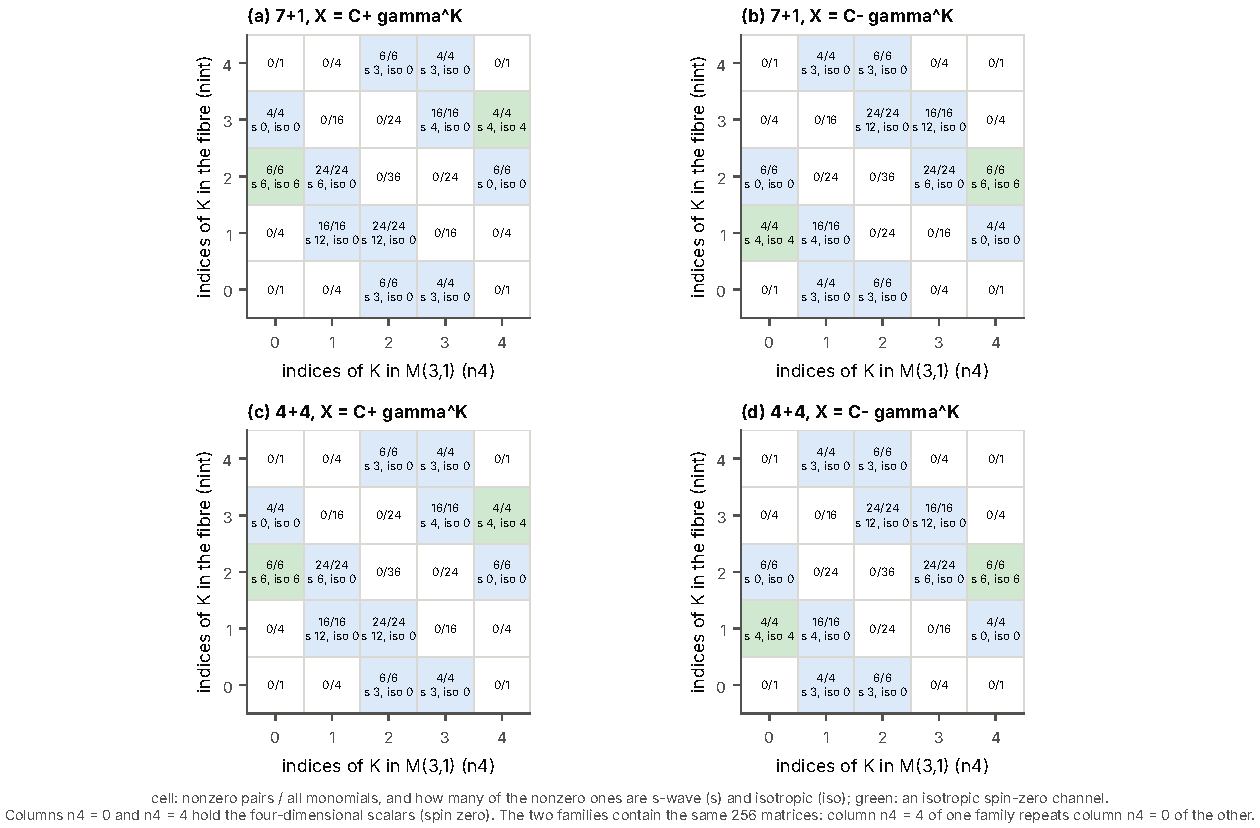
\includegraphics[width=0.85\textwidth]{../figures/fig_ng_channels.pdf}
\caption{All 512 one-field pair matrices $C^\pm_{\rm NG}\gamma^K_{\rm NG}$ on $7{+}1$ (a, b) and $4{+}4$ (c, d),
sorted by the number of indices of $K$ in the world (horizontal) and in the fibre (vertical). Each cell
gives the number of nonzero pairs among all products, and of these the numbers that are s-wave and
isotropic. Green: the isotropic spin-zero channels, Eq.~(\ref{eq:channels}). Data:
\texttt{data/ng\_pair\_channels.csv}.}
\label{fig:channels}
\end{figure*}

\subsection{The model}

We take the eight-dimensionally Lorentz-invariant interaction of the vector pairs,
\begin{equation}
\mathcal H^{\rm V}_{\rm NG}=\frac{G_{\rm NG}}4\sum_{A,B}\eta^{AB}_{1671}\,(\Delta^A_{1671})^\dagger\Delta^B_{1671}
\label{eq:hv}
\end{equation}
on $7{+}1$ (and the same with the tag 1644 on $4{+}4$), with a coupling $G_{\rm NG}>0$ of dimension
mass$^{-2}$ in the four-dimensional world, and restrict it to the fields of the world. On $7{+}1$ the
entries $\eta^{aa}_{1671}=\eta^{jj}_{1671}=-1$ make it attractive in the four spin-zero components
$\Delta^a_{1671}$ and in the three spin-one components $\Delta^j_{1671}$, all with the \emph{same}
coupling, and repulsive in the time component $\Delta^4_{1671}$. On $4{+}4$ it is attractive where
$\eta^{AA}_{1644}=-1$: in the spin-zero components $\Delta^t_{1644}$ ($t=5,6,7$) and in the time
component, which is not s-wave; it repels $\Delta^0_{1644}$ and the space components (check P-11). In
the attractive spin-zero channel the interaction is
\begin{equation}
\mathcal H^{\rm int}_{\rm NG}=-\frac{G_{\rm NG}}4\sum_a(\psi^T_{\rm NG}\mathsf K^a_{\rm NG}\psi_{\rm NG})^\dagger
(\psi^T_{\rm NG}\mathsf K^a_{\rm NG}\psi_{\rm NG})
\label{eq:hint}
\end{equation}
(on $4{+}4$ the sum runs over $t=5,6,7$ only). The same form with $\mathsf K^{ab}_{\rm NG}$ describes the
two-form channel, and $\mathcal H^{\rm D}_{\rm NG}=-\tfrac14G^{\rm D}_{\rm NG}(\Phi^{\rm D}_{\rm NG})^\dagger
\Phi^{\rm D}_{\rm NG}$, with its own coupling $G^{\rm D}_{\rm NG}$, the doublet channel. The mean-field
approximation replaces the product of two pairs by the products of each with the expectation value of
the other. With the pair amplitudes $\Delta^a_{\rm NG}=\tfrac12G_{\rm NG}\langle\psi^T_{\rm NG}
\mathsf K^a_{\rm NG}\psi_{\rm NG}\rangle$ (complex numbers),
\begin{align}
\mathcal H^{\rm MF}_{\rm NG}&=\psi^\dagger_{\rm NG}(\mathsf h_{\rm NG}-\mu_{\rm NG})\psi_{\rm NG}+\frac{\lvert\Delta_{\rm NG}\rvert^2}{G_{\rm NG}}\nonumber\\
&\quad-\tfrac12\sum_a\big(\Delta^{a*}_{\rm NG}\,\psi^T_{\rm NG}\mathsf K^a_{\rm NG}\psi_{\rm NG}+{\rm h.c.}\big),
\label{eq:hmf}
\end{align}
with $\lvert\Delta_{\rm NG}\rvert^2=\sum_a\lvert\Delta^a_{\rm NG}\rvert^2$ and the chemical potential
$\mu_{\rm NG}$ that fixes the density of fermions. The two-form amplitudes $\Delta^{ab}_{\rm NG}$ and the
doublet amplitude $\Delta^{\rm D}_{\rm NG}=\tfrac12G^{\rm D}_{\rm NG}\langle\Phi^{\rm D}_{\rm NG}\rangle$ are
defined in the same way.

\subsection{Bogoliubov-de Gennes spectrum}

With the Nambu spinor $\mathcal N_{\rm NG}(\vec q)=(\psi_{\rm NG}(\vec q),\psi_{\rm NG}(-\vec q)^{\dagger T})$ of
32 components, $\sum_{\vec q}\mathcal H^{\rm MF}_{\rm NG}=\tfrac12\sum_{\vec q}\mathcal N^\dagger_{\rm NG}
\mathsf H_{\rm NG}(\vec q)\mathcal N_{\rm NG}+\text{constant}$, with the Bogoliubov-de Gennes matrix
\begin{align}
\mathsf H_{\rm NG}(\vec q)&=\begin{pmatrix}\mathsf h_{\rm NG}(\vec q)-\mu_{\rm NG}&\mathsf P_{\rm NG}\\
\mathsf P_{\rm NG}^\dagger&-(\mathsf h_{\rm NG}(-\vec q)-\mu_{\rm NG})^T\end{pmatrix},\nonumber\\
\mathsf P_{\rm NG}&=-\sum_a\Delta^a_{\rm NG}(\mathsf K^a_{\rm NG})^\dagger.
\label{eq:bdg}
\end{align}
For the doublet the Nambu spinor is $(\psi^1_{\rm NG}(\vec q),\psi^2_{\rm NG}(-\vec q)^{\dagger T})$, the factor
$\tfrac12$ is absent, and $\mathsf P_{\rm NG}=\Delta^{\rm D}_{\rm NG}(C^+_{1671})^*$. The lower right block equals
$\mu_{\rm NG}-\beta_{1671}\mathsf h_{\rm NG}(\vec q)\beta_{1671}$ on $7{+}1$ and $\mathsf h_{\rm NG}(\vec q)+
\mu_{\rm NG}$ on $4{+}4$, by the symmetry properties of $\alpha^j_{\rm NG}$ and $\beta_{\rm NG}$ stated above.
The grand potential per volume at zero temperature, the \emph{effective potential} of the superfluid,
is the ground-state energy of $\mathcal H^{\rm MF}_{\rm NG}$ per volume:
\begin{equation}
\Omega_{\rm NG}=\frac{\lvert\Delta_{\rm NG}\rvert^2}{G_{\rm NG}}-\frac12\int\frac{d^3q}{(2\pi)^3}
\sum_{\mathcal E_{\rm NG}>0}\mathcal E_{\rm NG}(\vec q),
\label{eq:omega}
\end{equation}
summed over the positive eigenvalues $\mathcal E_{\rm NG}$ of $\mathsf H_{\rm NG}(\vec q)$, up to terms that do not
depend on the pair amplitudes. The factor $\tfrac12$ appears because each mode of one field occurs twice in
the Nambu spinor; for the doublet, whose Nambu spinor contains each mode once, it is absent (and
$G^{\rm D}_{\rm NG}$ replaces $G_{\rm NG}$).

\emph{Theorem 5 (isotropic gap).} Let $\mathsf P_{\rm NG}$ commute with $\beta_{\rm NG}$ (on $7{+}1$) or
anticommute with it (on $4{+}4$), anticommute with every $\alpha^j_{\rm NG}$, and satisfy
$\mathsf P_{\rm NG}\mathsf P_{\rm NG}^\dagger=\mathsf P^\dagger_{\rm NG}\mathsf P_{\rm NG}=\lvert\Delta_{\rm NG}\rvert^2\mathsf 1_{16}$.
Then the eigenvalues of $\mathsf H_{\rm NG}(\vec q)$ are $\pm E^+_{\rm NG}$ and $\pm E^-_{\rm NG}$, eight times
each, with
\begin{equation}
E^\pm_{\rm NG}=\big[(\varepsilon_{\rm NG}\pm\mu_{\rm NG})^2+\lvert\Delta_{\rm NG}\rvert^2\big]^{1/2}.
\label{eq:epm}
\end{equation}
\emph{Proof} (for $7{+}1$; on $4{+}4$ replace $\mu_{\rm NG}-\beta_{1671}\mathsf h_{\rm NG}\beta_{1671}$ by
$\mathsf h_{\rm NG}+\mu_{\rm NG}$ and use the anticommutation with $\beta_{1644}$). The off-diagonal block of
$\mathsf H_{\rm NG}^2$ is $(\mathsf h_{\rm NG}-\mu_{\rm NG})\mathsf P_{\rm NG}+\mathsf P_{\rm NG}(\mu_{\rm NG}-
\beta_{1671}\mathsf h_{\rm NG}\beta_{1671})=\mathsf h_{\rm NG}\mathsf P_{\rm NG}-\mathsf P_{\rm NG}\beta_{1671}
\mathsf h_{\rm NG}\beta_{1671}$; since $\beta_{1671}\mathsf h_{\rm NG}(\vec q)\beta_{1671}=-\sum_j\alpha^j_{1671}q^j+
\beta_{1671}m_{1671}$ and $\mathsf P_{\rm NG}$ anticommutes with the $\alpha^j_{1671}$ and commutes with
$\beta_{1671}$, $\mathsf P_{\rm NG}\beta_{1671}\mathsf h_{\rm NG}\beta_{1671}=\mathsf h_{\rm NG}\mathsf P_{\rm NG}$, and the
block vanishes. The diagonal blocks are $(\mathsf h_{\rm NG}-\mu_{\rm NG})^2+\lvert\Delta_{\rm NG}\rvert^2$ and
$(\mu_{\rm NG}-\beta_{1671}\mathsf h_{\rm NG}\beta_{1671})^2+\lvert\Delta_{\rm NG}\rvert^2$, each with the
eigenvalues $(\varepsilon_{\rm NG}+\mu_{\rm NG})^2+\lvert\Delta_{\rm NG}\rvert^2$ and $(\varepsilon_{\rm NG}-
\mu_{\rm NG})^2+\lvert\Delta_{\rm NG}\rvert^2$, eight times each. Hence $\mathsf H_{\rm NG}$ has the eigenvalues
$\pm E^+_{\rm NG}$, $\pm E^-_{\rm NG}$ with 16 eigenvalues of each modulus. $\mathsf H_{\rm NG}$ is traceless
(its diagonal blocks have the traces $\mathrm{tr}\,\mathsf h_{\rm NG}(\vec q)=0$ and
$-\mathrm{tr}\,\mathsf h_{\rm NG}(-\vec q)=0$, apart from $\mp16\mu_{\rm NG}$, which cancel). When
$E^+_{\rm NG}/E^-_{\rm NG}$ is irrational, a vanishing sum of the eigenvalues requires as many eigenvalues
$+E^\pm_{\rm NG}$ as $-E^\pm_{\rm NG}$, i.e.\ eight of each; the eigenvalues depend continuously on
$\mu_{\rm NG}$ and never pass through zero (they have moduli $E^\pm_{\rm NG}\ge\lvert\Delta_{\rm NG}\rvert>0$),
so the multiplicities are eight for all parameters. $\square$

The channels of Eq.~(\ref{eq:channels}) satisfy the hypotheses for every real direction of the pair
amplitudes (and every common phase): for real amplitudes the cross terms $\Delta^a_{\rm NG}\Delta^b_{\rm NG}$
of $\mathsf P_{\rm NG}\mathsf P_{\rm NG}^\dagger$ multiply the antisymmetric combinations $\gamma^a_{\rm NG}
\gamma^b_{\rm NG}+\gamma^b_{\rm NG}\gamma^a_{\rm NG}=0$ ($a\ne b$). The program confirms the spectrum on random
momenta, chemical potentials, masses and directions for the vector, two-form and doublet channels on
both spacetimes (check P-2). With Eq.~(\ref{eq:omega}) every isotropic state has
\begin{align}
\Omega_{\rm NG}&=\frac{\lvert\Delta_{\rm NG}\rvert^2}{G_{\rm NG}}-\nu_{\rm NG}\int\frac{d^3q}{(2\pi)^3}
\big(E^+_{\rm NG}+E^-_{\rm NG}\big),\nonumber\\
\frac1{G_{\rm NG}}&=\frac{\nu_{\rm NG}}2\int\frac{d^3q}{(2\pi)^3}
\Big(\frac1{E^+_{\rm NG}}+\frac1{E^-_{\rm NG}}\Big),
\label{eq:gap}
\end{align}
the second equation (the \emph{gap equation}) being the condition for a minimum away from zero, with
$\nu_{\rm NG}=4$ for one field and $\nu_{\rm NG}=8$ for the doublet (for which $G^{\rm D}_{\rm NG}$ replaces
$G_{\rm NG}$): eight positive eigenvalues of each kind, times $\tfrac12$ or 1. The program verifies the
first equation against the numerical sum over the eigenvalues of $\mathsf H_{\rm NG}$ (check P-5).
Throughout, the momentum integrals are cut off at $\lvert\vec q\rvert=\Lambda_{\rm NG}$, and we set
$\Lambda_{\rm NG}=1$.

\emph{Non-unitary and spin-one states.} For the complex direction $\Delta^0_{\rm NG}=\lvert\Delta_{\rm NG}
\rvert\cos\upsilon_{\rm NG}$, $\Delta^5_{\rm NG}=i\lvert\Delta_{\rm NG}\rvert\sin\upsilon_{\rm NG}$,
$\Delta^6_{\rm NG}=\Delta^7_{\rm NG}=0$ of the vector amplitudes on $7{+}1$, with an angle $\upsilon_{\rm NG}$,
the cross terms no longer cancel. With $C^-_{1671}$ orthogonal and the $\gamma^a_{1671}$ real,
antisymmetric and of square $-\mathsf 1_{16}$, $(\mathsf K^a_{\rm NG})^\dagger\mathsf K^b_{\rm NG}=
-\gamma^a_{1671}\gamma^b_{1671}$, and one finds
$\mathsf P_{\rm NG}\mathsf P^\dagger_{\rm NG}=\lvert\Delta_{\rm NG}\rvert^2(\mathsf 1_{16}+\sin2\upsilon_{\rm NG}\,
i\gamma^0_{1671}\gamma^5_{1671})$ and $\mathsf P^\dagger_{\rm NG}\mathsf P_{\rm NG}=\lvert\Delta_{\rm NG}\rvert^2(\mathsf 1_{16}-
\sin2\upsilon_{\rm NG}\,i\gamma^0_{1671}\gamma^5_{1671})$, where $i\gamma^0_{1671}\gamma^5_{1671}$ is
Hermitian, has square $\mathsf 1_{16}$, and commutes with $\alpha^j_{1671}$ and $\beta_{1671}$. The
off-diagonal block of $\mathsf H_{\rm NG}^2$ still vanishes, and on the eigenspaces of $i\gamma^0_{1671}\gamma^5_{1671}$ the
gap splits into $\lvert\Delta_{\rm NG}\rvert(1\pm\zeta_{\rm NG})^{1/2}$, $\zeta_{\rm NG}=\lvert\sin
2\upsilon_{\rm NG}\rvert$, still independent of the direction of motion (check P-3a, which also confirms
the multiplicities, four each); the \emph{chiral} state $\upsilon_{\rm NG}=\pi/4$ has the gaps
$\sqrt2\lvert\Delta_{\rm NG}\rvert$ and 0. The spin-one pair $C^-_{\rm NG}\gamma^1_{\rm NG}$ (direction
$\hat n_{\rm NG}$ along $x1$) commutes with $\alpha^1_{\rm NG}$ instead of anticommuting with it, and its
spectrum is (check P-4)
\begin{align}
(E^{(1)\pm}_{\rm NG})^2&=\varepsilon_{\rm NG}^2+\mu_{\rm NG}^2+\lvert\Delta_{\rm NG}\rvert^2\nonumber\\
&\quad\pm2\big[\mu_{\rm NG}^2\varepsilon_{\rm NG}^2+\lvert\Delta_{\rm NG}\rvert^2(q^1)^2\big]^{1/2},
\label{eq:spin1}
\end{align}
eight times each, which depends on the angle between $\vec q$ and $\hat n_{\rm NG}$. For $\vec q$ along
$\hat n_{\rm NG}$ on the Fermi surface $\varepsilon_{\rm NG}=\mu_{\rm NG}$, the lower energy is
$\lvert\Delta_{\rm NG}\rvert m_{\rm NG}/\mu_{\rm NG}$ to leading order in $\lvert\Delta_{\rm NG}\rvert$; for
massless fermions $(E^{(1)-}_{\rm NG})^2=(q-(\mu_{\rm NG}^2+\lvert\Delta_{\rm NG}\rvert^2)^{1/2})^2$ along
$\hat n_{\rm NG}$, which vanishes exactly at $q=(\mu_{\rm NG}^2+\lvert\Delta_{\rm NG}\rvert^2)^{1/2}$.

\subsection{Vacuum and finite density}

\emph{Vacuum.} At $\mu_{\rm NG}=0$ a pair condensate forms only if the gap equation~(\ref{eq:gap}) has a
solution, i.e.\ above the critical coupling $G^{\rm crit}_{\rm NG}$ with $1/G^{\rm crit}_{\rm NG}=\nu_{\rm NG}
\int d^3q\,(2\pi)^{-3}\varepsilon_{\rm NG}^{-1}$ (the right side of the gap equation at
$\lvert\Delta_{\rm NG}\rvert\to0$, which is its largest value); for massless fermions $\int d^3q\,
(2\pi)^{-3}q^{-1}=\Lambda_{\rm NG}^2/(4\pi^2)$ and $G^{\rm crit}_{\rm NG}=4\pi^2/(\nu_{\rm NG}
\Lambda_{\rm NG}^2)$: $\pi^2/\Lambda_{\rm NG}^2$ for one field and $\pi^2/(2\Lambda_{\rm NG}^2)$ for the doublet
(the program finds $9.8696044011$ and $4.9348022005$; for $m_{\rm NG}=0.2$ the one-field value
is $10.643305$; check P-6, Fig.~\ref{fig:gap}). The vacuum condensate is a four-dimensional
Lorentz scalar, so the vacuum of the world stays Lorentz invariant.

\begin{figure}[t]
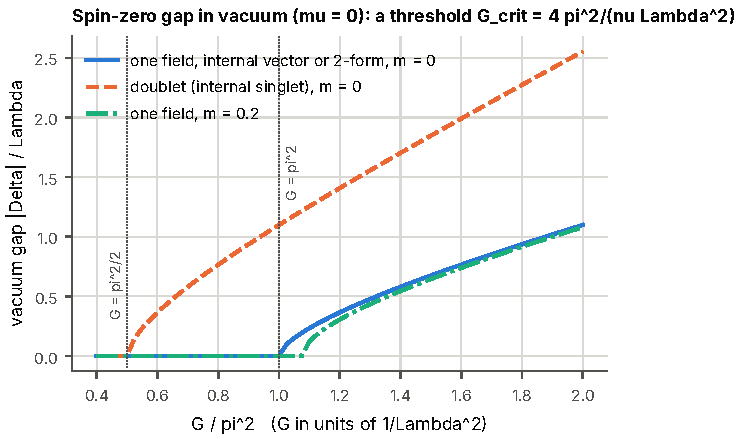
\includegraphics[width=\columnwidth]{../figures/fig_ng_gap.pdf}
\caption{Gap of the vacuum versus coupling. A single field condenses in the internal-vector or
two-form channel above $G_{\rm NG}=\pi^2$ ($m_{\rm NG}=0$; blue) or slightly above it ($m_{\rm NG}=0.2$;
aqua); the doublet (orange) above $\pi^2/2$. Units: $\Lambda_{\rm NG}=1$; gaps of order
$\Lambda_{\rm NG}$ and more lie outside the range in which a model with a cutoff is meaningful. Data:
\texttt{data/ng\_gap\_vs\_coupling.csv}.}
\label{fig:gap}
\end{figure}

\emph{Finite density.} For $\mu_{\rm NG}>m_{\rm NG}$ there is a Fermi surface at
$q=q^{\rm F}_{\rm NG}=(\mu_{\rm NG}^2-m_{\rm NG}^2)^{1/2}$, where $E^-_{\rm NG}$ becomes as small as
$\lvert\Delta_{\rm NG}\rvert$; the integral of $1/E^-_{\rm NG}$ then grows like $\ln(1/\lvert\Delta_{\rm NG}
\rvert)$, and the gap equation has a solution for every attraction (Cooper instability~\cite{BCS1957}).
Near the Fermi surface $d^3q/(2\pi)^3=q^2dq/(2\pi^2)$ and $q\,dq=\varepsilon_{\rm NG}d\varepsilon_{\rm NG}$
give $d^3q/(2\pi)^3\approx q^{\rm F}_{\rm NG}\mu_{\rm NG}\,d\varepsilon_{\rm NG}/(2\pi^2)$, so at weak coupling
$\ln\lvert\Delta_{\rm NG}\rvert=\text{constant}-2\pi^2/(\nu_{\rm NG}q^{\rm F}_{\rm NG}\mu_{\rm NG}G_{\rm NG})$. The
program finds a gap for a coupling that is subcritical in the vacuum, none below $\mu_{\rm NG}=m_{\rm NG}$,
and a slope of $\ln\lvert\Delta_{\rm NG}\rvert$ against $1/G_{\rm NG}$ equal to $0.9945$ times the
predicted one (check P-7, Fig.~\ref{fig:density}).

\begin{figure*}[t]
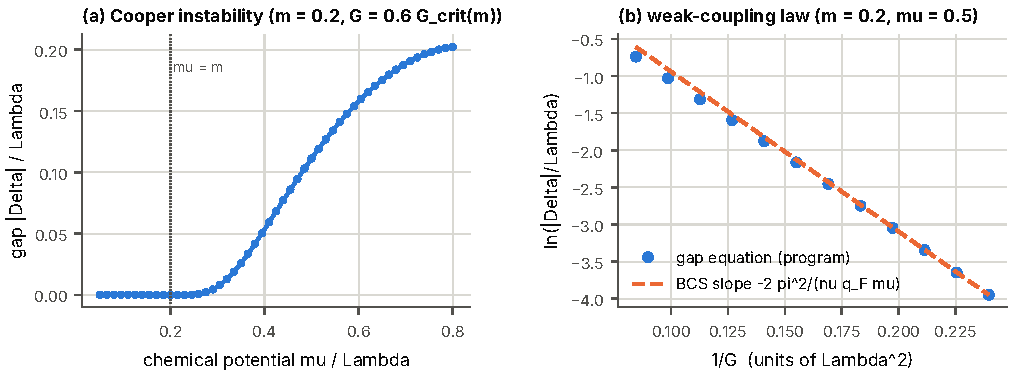
\includegraphics[width=0.92\textwidth]{../figures/fig_ng_density.pdf}
\caption{(a) The gap versus the chemical potential for a coupling below the vacuum threshold: it appears
when a Fermi surface exists. (b) At weak coupling the logarithm of the gap falls linearly in
$1/G_{\rm NG}$ with the slope $-2\pi^2/(\nu_{\rm NG}q^{\rm F}_{\rm NG}\mu_{\rm NG})$ (dashed). Data:
\texttt{data/ng\_gap\_vs\_mu.csv}, \texttt{data/ng\_bcs\_law.csv}.}
\label{fig:density}
\end{figure*}

\subsection{Which state wins}

The interaction~(\ref{eq:hv}) treats the four spin-zero and the three spin-one components of the vector
pairs on $7{+}1$ alike. The ground state is nevertheless the polar spin-zero state: \emph{at every
amplitude $\lvert\Delta_{\rm NG}\rvert$, $\Omega_{\rm NG}$ is lowest for the isotropic (polar) state.} For the
non-unitary states the two gaps $\lvert\Delta_{\rm NG}\rvert(1\pm\zeta_{\rm NG})^{1/2}$ have the mean square
$\lvert\Delta_{\rm NG}\rvert^2$, and the square root is concave, so with $\xi_{\rm NG}=\varepsilon_{\rm NG}\pm
\mu_{\rm NG}$, $\sum_\pm[\xi_{\rm NG}^2+\lvert\Delta_{\rm NG}\rvert^2(1\pm\zeta_{\rm NG})]^{1/2}\le
2[\xi_{\rm NG}^2+\lvert\Delta_{\rm NG}\rvert^2]^{1/2}$ at every momentum, and the subtracted integral in
Eq.~(\ref{eq:omega}) is smaller. For the spin-one state the sum of the squares of the two energies of
Eq.~(\ref{eq:spin1}) is the same as for the polar state, $2(\varepsilon_{\rm NG}^2+\mu_{\rm NG}^2+
\lvert\Delta_{\rm NG}\rvert^2)$, but the square of their product is smaller by $4\lvert\Delta_{\rm NG}\rvert^2
(q^1)^2$, so their sum $[(E^{(1)+}_{\rm NG})^2+(E^{(1)-}_{\rm NG})^2+2E^{(1)+}_{\rm NG}E^{(1)-}_{\rm NG}]^{1/2}$ is
smaller. The program confirms the order at all 60 amplitudes of its grid (check P-8,
Fig.~\ref{fig:states}): at $m_{\rm NG}=0.2$, $\mu_{\rm NG}=0.5$ and $G_{\rm NG}=0.9\,G^{\rm crit}_{\rm NG}$ (the
critical coupling for $m_{\rm NG}=0.2$) the smallest values of $\Omega_{\rm NG}$ on the grid are
$-2.505051$ (polar
spin zero), $-1.252231$ (chiral) and $-0.4971294$ (spin one), in units of
$10^{-3}\Lambda_{\rm NG}^4$, and the polar gap is $0.317478$.

\begin{figure*}[t]
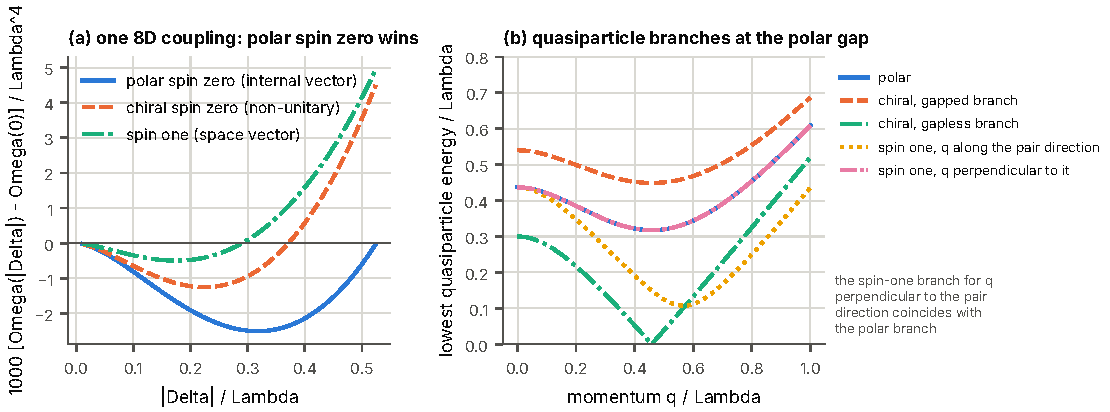
\includegraphics[width=0.92\textwidth]{../figures/fig_ng_states.pdf}
\caption{(a) Effective potential of the polar spin-zero, chiral spin-zero and spin-one states for one
eight-dimensional coupling ($m_{\rm NG}=0.2$, $\mu_{\rm NG}=0.5$, $G_{\rm NG}=0.9\,G^{\rm crit}_{\rm NG}$). (b)
Lowest quasi-particle energies at the polar gap: the polar branch, the two branches of the chiral state
(one gapless), and the spin-one branch along and perpendicular to the direction of the pair. Data:
\texttt{data/ng\_omega\_states.csv}, \texttt{data/ng\_dispersion.csv}.}
\label{fig:states}
\end{figure*}

\subsection{The amplitude mode}

By the proof of Theorem~5, each isotropic channel decomposes into independent pairs of a particle and a
hole with the $2\times2$ matrices $\big(\begin{smallmatrix}\xi_{\rm NG}&\lvert\Delta_{\rm NG}\rvert\\
\lvert\Delta_{\rm NG}\rvert&-\xi_{\rm NG}\end{smallmatrix}\big)$, $\xi_{\rm NG}=\varepsilon_{\rm NG}\pm
\mu_{\rm NG}$, as in the theory of Bardeen, Cooper and Schrieffer. Let the amplitude oscillate,
$\lvert\Delta_{\rm NG}\rvert\to\lvert\Delta_{\rm NG}\rvert+\delta_{\rm NG}\exp(-iw_{\rm NG}x4)$ with a small real
$\delta_{\rm NG}$ and a frequency $w_{\rm NG}$. In each block it couples to the off-diagonal matrix
$\big(\begin{smallmatrix}0&1\\1&0\end{smallmatrix}\big)$, whose matrix element between the two eigenstates
of energy $\pm E^\pm_{\rm NG}$ has the square $\xi_{\rm NG}^2/(E^\pm_{\rm NG})^2$; the linear response of
the pair amplitude then gives the inverse propagator of the oscillation (random-phase approximation),
\begin{align}
\Pi^{\rm A}_{\rm NG}(w_{\rm NG})&=\frac1{G_{\rm NG}}\nonumber\\
&\quad-\frac{\nu_{\rm NG}}2\int\frac{d^3q}{(2\pi)^3}\sum_\pm
\frac{4(\varepsilon_{\rm NG}\pm\mu_{\rm NG})^2}{E^\pm_{\rm NG}[4(E^\pm_{\rm NG})^2-w_{\rm NG}^2]},
\label{eq:pia}
\end{align}
a mode existing where it vanishes. Eliminating $1/G_{\rm NG}$ with the gap equation and using
$(E^\pm_{\rm NG})^2-(\varepsilon_{\rm NG}\pm\mu_{\rm NG})^2=\lvert\Delta_{\rm NG}\rvert^2$ gives
\begin{align}
\Pi^{\rm A}_{\rm NG}(w_{\rm NG})&=(4\lvert\Delta_{\rm NG}\rvert^2-w_{\rm NG}^2)\,c^\sigma_{\rm NG}(w_{\rm NG}),\nonumber\\
c^\sigma_{\rm NG}(w_{\rm NG})&=\frac{\nu_{\rm NG}}2\int\frac{d^3q}{(2\pi)^3}\sum_\pm\frac1{E^\pm_{\rm NG}
[4(E^\pm_{\rm NG})^2-w_{\rm NG}^2]},
\label{eq:csigma}
\end{align}
and $c^\sigma_{\rm NG}$ is finite and positive for $0\le w_{\rm NG}\le2\lvert\Delta_{\rm NG}\rvert$ in the
vacuum (there $E^\pm_{\rm NG}\ge\lvert\Delta_{\rm NG}\rvert$, and near the minimum the factor $q^2$ of the
volume element cancels the zero of the denominator). Hence the amplitude (Higgs) mode has the mass
$m^\sigma_{\rm NG}=2\lvert\Delta_{\rm NG}\rvert$ exactly, at the threshold for breaking a pair. The program
evaluates $c^\sigma_{\rm NG}$ on $[0,2\lvert\Delta_{\rm NG}\rvert]$ for $m_{\rm NG}=0$, $G_{\rm NG}=1.5\pi^2$, where
$\lvert\Delta_{\rm NG}\rvert=$$0.6753386910$, and checks the static limit: $\Pi^{\rm A}_{\rm NG}(0)$ must
equal half the second derivative of $\Omega_{\rm NG}$ with respect to $\lvert\Delta_{\rm NG}\rvert$ at the
minimum, and the two numbers are $3.28385662\times10^{-2}$ and $3.28385662\times10^{-2}$ (check P-9,
Fig.~\ref{fig:amplitude}). For an oscillation of the phase, the matrix element squared is 1 instead of
$\xi_{\rm NG}^2/(E^\pm_{\rm NG})^2$, and the same steps give the inverse propagator
$-w_{\rm NG}^2\,c^\sigma_{\rm NG}(w_{\rm NG})$, which vanishes at $w_{\rm NG}=0$: the phase oscillation is a
Goldstone mode (derived here, not machine-checked).

\begin{figure}[t]
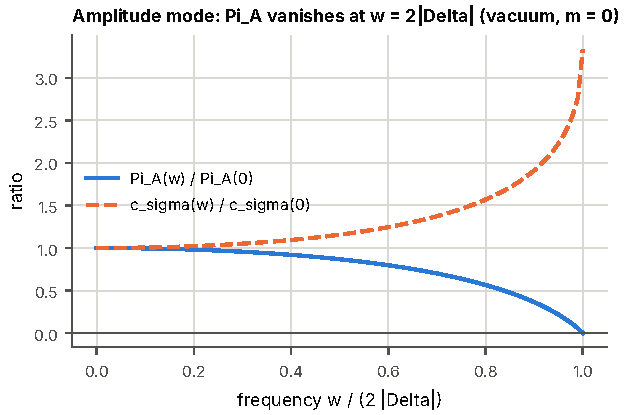
\includegraphics[width=\columnwidth]{../figures/fig_ng_amplitude.pdf}
\caption{The amplitude mode in the vacuum ($m_{\rm NG}=0$, $G_{\rm NG}=1.5\pi^2$): the inverse propagator
$\Pi^{\rm A}_{\rm NG}$ vanishes at $w_{\rm NG}=2\lvert\Delta_{\rm NG}\rvert$, where $c^\sigma_{\rm NG}$ is still
finite. Data: \texttt{data/ng\_amplitude\_mode.csv}.}
\label{fig:amplitude}
\end{figure}

\subsection{Spontaneous breaking and the locking of a Lorentz rotation to the fermion number}

On $7{+}1$ the one-field theory is symmetric under the Lorentz group of the world, the rotations of the
fibre and the fermion number. We denote by $\mathcal T^{ab}_{\rm NG}$ ($a<b$) the generator of rotations of
the fibre in the plane of $xa$ and $xb$; on the vector amplitudes it acts by changing $\Delta^a_{\rm NG}$ by
$-\Delta^b_{\rm NG}$ and $\Delta^b_{\rm NG}$ by $+\Delta^a_{\rm NG}$ per unit parameter (and on the two-form
amplitudes as on the products of two vectors). The fermion number $\psi_{\rm NG}\to\exp(i\varphi_{\rm NG})
\psi_{\rm NG}$ multiplies every pair by $\exp(2i\varphi_{\rm NG})$; its generator $F_{\rm NG}$ multiplies every
pair amplitude by $2i$. The condensates are scalars of the world, so its Lorentz group stays unbroken;
the symmetry of the fibre and of the fermion number, a group of dimension 7, is broken to the stabilizer
of the condensate, which the program computes exactly (check P-10, Fig.~\ref{fig:goldstone}):
\begin{itemize}
\item polar vector, only $\Delta^0_{\rm NG}\neq0$: unbroken rotations of $x5,x6,x7$ (dimension 3); four
broken generators;
\item chiral vector, $\Delta^5_{\rm NG}=i\Delta^0_{\rm NG}$ and $\Delta^6_{\rm NG}=\Delta^7_{\rm NG}=0$: unbroken
$\mathcal T^{05}_{\rm NG}+\tfrac12F_{\rm NG}$ and $\mathcal T^{67}_{\rm NG}$ (dimension 2); five broken generators;
\item self-dual two-form, $\Delta^{05}_{\rm NG}=\Delta^{67}_{\rm NG}$ and all other components zero: unbroken
$U(1)\times SU(2)$ (dimension 4); three broken generators.
\end{itemize}
For the chiral state, $\mathcal T^{05}_{\rm NG}$ changes $(\Delta^0_{\rm NG},\Delta^5_{\rm NG})=(1,i)\Delta^0_{\rm NG}$
by $(-i,1)\Delta^0_{\rm NG}=-i(1,i)\Delta^0_{\rm NG}$, and $\tfrac12F_{\rm NG}$ by $+i(1,i)\Delta^0_{\rm NG}$, so their
sum leaves it unchanged. The unbroken generator $\mathcal T^{05}_{\rm NG}+\tfrac12F_{\rm NG}$ is the sum of a
rotation in the plane of $x0$ and $x5$---an element of the eight-dimensional Lorentz group---and the
fermion number: \emph{a Lorentz rotation of eight dimensions is locked to an internal charge in the
symmetry of a four-dimensionally Lorentz-invariant vacuum.} In four dimensions this is allowed, because
the rotation of the fibre is an internal symmetry there; in eight dimensions it is possible because the
combined manifold breaks the eight-dimensional Poincar\'e group (H1). Seen in eight dimensions, a polar
vector condensate is a vector of the Lorentz group pointing into the fibre; its stabilizer in
$\mathfrak{so}(7,1)$ is $\mathfrak{so}(6,1)$, of dimension 21, and 12 of its generators mix the world with
the fibre (check K-10). (At finite density, two broken generators whose commutator has a nonzero
expectation value give one Goldstone mode with quadratic dispersion instead of two; we count broken
generators and do not analyse the dispersions.)

\begin{figure}[t]
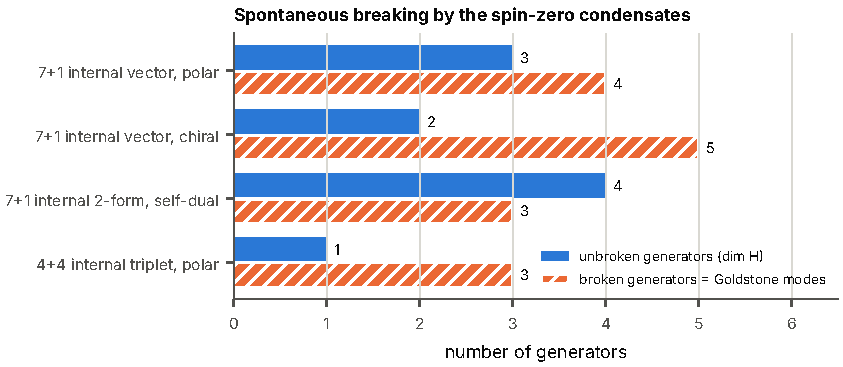
\includegraphics[width=\columnwidth]{../figures/fig_ng_goldstone.pdf}
\caption{Unbroken and broken generators of the spin-zero phases. Data: \texttt{data/ng\_goldstone.csv}.}
\label{fig:goldstone}
\end{figure}

\subsection{The superfluid on 4+4}

\emph{Theorem 6 (Wick map).} For every complex vector amplitude, the eigenvalues of the $4{+}4$ matrix
$\mathsf H_{\rm NG}(\vec q)$ equal those of the $7{+}1$ matrix with $\Delta^0_{\rm NG}$ replaced by
$i\Delta^0_{\rm NG}$; for the two-form channel, with $\Delta^{0t}_{\rm NG}$ replaced by $i\Delta^{0t}_{\rm NG}$.

\emph{Why.} For every complex amplitude $\mathsf P_{\rm NG}$ anticommutes with the $\alpha^j_{\rm NG}$ and
commutes (on $7{+}1$) or anticommutes (on $4{+}4$) with $\beta_{\rm NG}$, so, as in the proof of Theorem~5,
$\mathsf H_{\rm NG}^2$ is block diagonal; its blocks are a kinetic part with the eigenvalues
$(\varepsilon_{\rm NG}\pm\mu_{\rm NG})^2$, eight times each, plus $\mathsf P_{\rm NG}\mathsf P^\dagger_{\rm NG}$ or
$\mathsf P^\dagger_{\rm NG}\mathsf P_{\rm NG}$. These two products are combinations of $\mathsf 1_{16}$ and the
products $\gamma^a_{\rm NG}\gamma^b_{\rm NG}$ of fibre matrices, with coefficients quadratic in the
amplitudes. The products act on the fibre factor of $\mathbb C^4\otimes\mathbb C^4$ (check K-3) and commute
with the kinetic part, which acts on the world factor; the spectrum of $\mathsf H^2_{\rm NG}$ is therefore
fixed by the algebraic relations and the Hermiticity of the fibre matrices, and by the coefficients. On
$7{+}1$ the four fibre matrices are anti-Hermitian with square $-\mathsf 1_{16}$. On $4{+}4$ the three
$\gamma^t_{1644}$ are, but $\gamma^0_{1644}$ is Hermitian with square $+\mathsf 1_{16}$; the matrix
$i\gamma^0_{1644}$ is anti-Hermitian with square $-\mathsf 1_{16}$, and $\Delta^0_{\rm NG}(C^-_{1644}
\gamma^0_{1644})^\dagger=(i\Delta^0_{\rm NG})(C^-_{1644}\,i\gamma^0_{1644})^\dagger$. Hence the $4{+}4$
amplitudes $(\Delta^0_{\rm NG},\Delta^t_{\rm NG})$ enter exactly as the $7{+}1$ amplitudes $(i\Delta^0_{\rm NG},
\Delta^t_{\rm NG})$, and the spectra of $\mathsf H^2_{\rm NG}$ coincide. The square does not fix the signs of
the eigenvalues of $\mathsf H_{\rm NG}$; the program confirms that the full spectra coincide, for random
complex amplitudes and momenta, to rounding accuracy (check P-3b).

Hence the $4{+}4$ superfluid with a positive-definite norm is the $7{+}1$ superfluid with the fibre
direction $x0$ rotated to imaginary values: it has the compact fibre symmetry $\mathfrak{so}(4)$ of
Sec.~\ref{sec:combined} (generated by $\Sigma^{st}_{1644}$ and $i\Sigma^{0t}_{1644}$), not the non-compact
$\mathfrak{so}(1,3)$, which Theorem~3 excludes. The interaction~(\ref{eq:hv}) of $4{+}4$ breaks even the
compact symmetry to the rotations of $x5,x6,x7$: it attracts only the triplet $\Delta^t_{1644}$, whose
polar condensate breaks $U(1)\times SO(3)$ to $SO(2)$, with three broken generators (check P-10).

\section{Does the combined manifold cure non-renormalizability?}
\label{sec:renorm}

\subsection{Power counting}

With $\hbar=1$ and the speed of light 1, every quantity has a mass dimension, written in square
brackets. Let $D$ be the number of space dimensions in which the fields carry momentum (the symbol of
the project with this meaning): $D=7$ on the eight-dimensional spacetimes, $D=3$ in the
four-dimensional world. The action is dimensionless, so the Lagrangian density has dimension $D+1$,
and its kinetic terms fix the dimension of a fermion field to $D/2$ and of a scalar or gauge field to
$(D-1)/2$. The couplings then have the dimensions of Table~\ref{tab:powercount}: a gauge or Yukawa
coupling $(3-D)/2$, a quartic scalar coupling $3-D$, and a four-fermion contact coupling, such as
$G_{\rm NG}$ of Eq.~(\ref{eq:hv}), $1-D$ (check R-1). For $D=7$ every interaction has a coupling of
negative mass dimension.

\begin{table}[t]
\caption{Mass dimensions of fields and couplings for $D$ space dimensions (exact; data
\texttt{data/ng\_power\_counting.csv}).}
\label{tab:powercount}
\begin{ruledtabular}
\begin{tabular}{lccc}
& general $D$ & $D=3$ & $D=7$\\
\hline
fermion field & $D/2$ & $3/2$ & $7/2$\\
scalar or gauge field & $(D-1)/2$ & $1$ & $3$\\
gauge or Yukawa coupling & $(3-D)/2$ & $0$ & $-2$\\
quartic scalar coupling & $3-D$ & $0$ & $-4$\\
four-fermion coupling & $1-D$ & $-2$ & $-6$\\
\end{tabular}
\end{ruledtabular}
\end{table}

A coupling of negative dimension makes a theory non-renormalizable: the superficial degree of
divergence of a one-particle-irreducible graph, the power of the cutoff with which the graph grows
when all its loop momenta are large, is
\begin{align}
\deg_{\rm NG}&=(D+1)-\frac D2e^{\rm F}_{\rm NG}-\frac{D-1}2e^{\rm B}_{\rm NG}\nonumber\\
&\quad-\sum_{\rm vertices}[\text{coupling of the vertex}],
\label{eq:degree}
\end{align}
with $e^{\rm F}_{\rm NG}$ and $e^{\rm B}_{\rm NG}$ the numbers of external fermion and boson lines; it
grows without bound with the number of vertices when a coupling has negative dimension, and infinitely
many counterterms are needed. For the four-point function of the four-fermion interaction
($e^{\rm F}_{\rm NG}=4$, $e^{\rm B}_{\rm NG}=0$) with $\mathcal V_{\rm NG}$ vertices, Eq.~(\ref{eq:degree})
gives $\deg_{\rm NG}=(\mathcal V_{\rm NG}-1)(D-1)$: for $D=3$ it is 2 at one loop---the quadratic
growth with $\Lambda_{\rm NG}$ of the gap equation~(\ref{eq:gap})---and it grows with
$\mathcal V_{\rm NG}$, so the four-fermion model of Sec.~\ref{sec:superfluid} is non-renormalizable
already in four dimensions, like the model of Nambu and Jona-Lasinio~\cite{NambuJonaLasinio1961}: an
effective theory valid below its cutoff $\Lambda_{\rm NG}$. For $D=7$ it is $6(\mathcal V_{\rm NG}-1)$. For
the vertex function of a Yukawa coupling ($e^{\rm F}_{\rm NG}=2$, $e^{\rm B}_{\rm NG}=1$) it is
$\tfrac12(3-D)(1-\mathcal V_{\rm NG})$: 0 for every $\mathcal V_{\rm NG}$ when $D=3$ (renormalizable), and
growing by 2 per vertex when $D=7$ (check R-2, Fig.~\ref{fig:renorm}b).

\begin{figure*}[t]
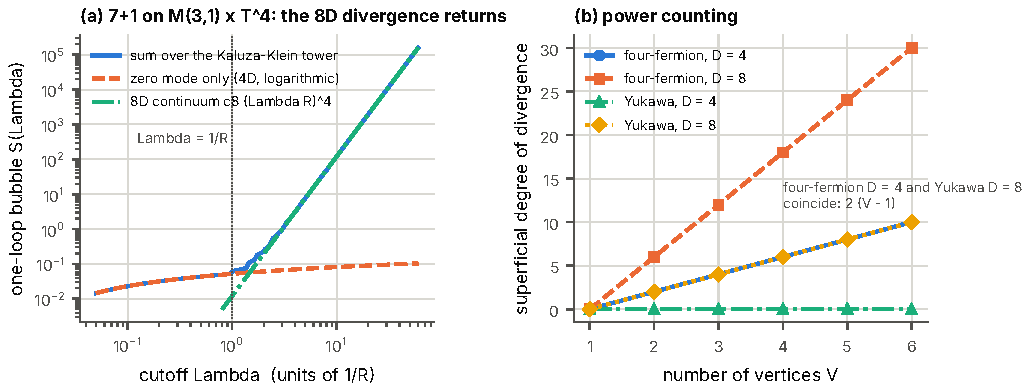
\includegraphics[width=0.92\textwidth]{../figures/fig_ng_renorm.pdf}
\caption{(a) The one-loop bubble on $7{+}1$ with a torus fibre of radius $R_{\rm NG}$ ($m_{\rm NG}R_{\rm NG}=0.01$),
summed over the Kaluza-Klein tower ($\mathcal B_{\rm NG}$, blue), compared with the bubble of the zero
mode alone ($f_{\rm NG}$, orange; logarithmic, four-dimensional) and with the eight-dimensional form
$\mathcal C^{(8)}_{\rm NG}(\Lambda_{\rm NG}R_{\rm NG})^4$ (green). Above $\Lambda_{\rm NG}=1/R_{\rm NG}$ the
eight-dimensional divergence returns. (b) The superficial degree of divergence $\deg_{\rm NG}$ versus the
number $\mathcal V_{\rm NG}$ of vertices. In the figure, B, f, C8, Lambda, R and nvert are
$\mathcal B_{\rm NG}$, $f_{\rm NG}$, $\mathcal C^{(8)}_{\rm NG}$, $\Lambda_{\rm NG}$, $R_{\rm NG}$ and
$\mathcal V_{\rm NG}$, and M(3,1) x T\^{}4 is the combined manifold with a torus fibre. Data:
\texttt{data/ng\_kk\_bubble.csv}, \texttt{data/ng\_superficial\_degree.csv}.}
\label{fig:renorm}
\end{figure*}

\subsection{A geometric fibre: the Kaluza-Klein tower}

If the fibre is a torus of radius $R_{\rm NG}$ on which the fields depend, each field of $7{+}1$ is a tower of
four-dimensional fields with the masses $(m^{\rm eff}_{\rm NG})^2=m_{1671}^2+\ell_{\rm NG}/R_{\rm NG}^2$ of
Eq.~(\ref{eq:kkmass}), where $\ell_{\rm NG}=\sum_a(n^a_{\rm NG})^2$ is the squared length of the integer
vector $(n^0_{\rm NG},n^5_{\rm NG},n^6_{\rm NG},n^7_{\rm NG})$. The number of integer vectors of squared length
$\ell_{\rm NG}$ is given by Jacobi's four-square theorem: $\mathrm r_4(\ell_{\rm NG})=8$ times the sum of the
divisors of $\ell_{\rm NG}$ that are not multiples of 4, and $\mathrm r_4(0)=1$ (check R-3 compares it with
a direct count). As a measure of the divergences we take the one-loop bubble of one four-dimensional
field of mass $m^{\rm eff}_{\rm NG}$, the integral over the Euclidean four-momentum $\varkappa_{\rm NG}$ of the
world (cut off at $\Lambda_{\rm NG}$) of the product of two propagators,
\begin{align}
&f_{\rm NG}\big((m^{\rm eff}_{\rm NG})^2\big)=\int_{\varkappa_{\rm NG}<\Lambda_{\rm NG}}\frac{d^4\varkappa_{\rm NG}}{(2\pi)^4}
\frac1{(\varkappa^2_{\rm NG}+(m^{\rm eff}_{\rm NG})^2)^2}\nonumber\\
&\ =\frac1{16\pi^2}\Big[\ln\Big(1+\frac{\Lambda_{\rm NG}^2}
{(m^{\rm eff}_{\rm NG})^2}\Big)-\frac{\Lambda_{\rm NG}^2}{\Lambda_{\rm NG}^2+(m^{\rm eff}_{\rm NG})^2}\Big],
\label{eq:bubble}
\end{align}
which grows only logarithmically, $\Lambda_{\rm NG}\,df_{\rm NG}/d\Lambda_{\rm NG}=2\Lambda_{\rm NG}^4/[16\pi^2
(\Lambda_{\rm NG}^2+(m^{\rm eff}_{\rm NG})^2)^2]\to1/(8\pi^2)$: the divergence of a dimensionless coupling in four
dimensions. Summed over the tower up to the cutoff, i.e.\ over $\ell_{\rm NG}\le(\Lambda_{\rm NG}R_{\rm NG})^2$,
\begin{equation}
\mathcal B_{\rm NG}(\Lambda_{\rm NG})=\sum_{\ell_{\rm NG}}\mathrm r_4(\ell_{\rm NG})\,
f_{\rm NG}\big(m_{1671}^2+\ell_{\rm NG}/R_{\rm NG}^2\big).
\label{eq:tower}
\end{equation}
For $\Lambda_{\rm NG}<1/R_{\rm NG}$ only the zero mode contributes, and $\mathcal B_{\rm NG}$ is the
logarithmic bubble of four dimensions (check R-4: its logarithmic slope at $\Lambda_{\rm NG}=0.3/R_{\rm NG}$
is $0.99778$ times $1/(8\pi^2)$). For $\Lambda_{\rm NG}\gg1/R_{\rm NG}$ the sum over integer
vectors becomes $R^4_{\rm NG}$ times an integral over the fibre momentum, whose four-dimensional volume
element is $2\pi^2$ times the cube of its length times its differential; with
$\varpi_{\rm NG}$ the ratio of that length to $\Lambda_{\rm NG}$, and for $m_{1671}\to0$,
\begin{align}
\mathcal B_{\rm NG}&\to(\Lambda_{\rm NG}R_{\rm NG})^4\,\mathcal C^{(8)}_{\rm NG},\nonumber\\
\mathcal C^{(8)}_{\rm NG}&=\frac18\int_0^1d\varpi_{\rm NG}\,\varpi_{\rm NG}^3\Big[\ln\big(1+\varpi_{\rm NG}^{-2}\big)
-\frac1{1+\varpi_{\rm NG}^2}\Big]\nonumber\\
&=1.207170\times10^{-2},
\label{eq:c8}
\end{align}
the quartic divergence of the bubble in eight dimensions, whose integrand falls off only like the
inverse fourth power of the eight-dimensional momentum. The program finds
$\mathcal B_{\rm NG}/(\Lambda_{\rm NG}R_{\rm NG})^4=$$1.207225\times10^{-2}$ at $\Lambda_{\rm NG}R_{\rm NG}=60$ (ratio
$1.0000$ to $\mathcal C^{(8)}_{\rm NG}$; check R-4, Fig.~\ref{fig:renorm}a). Below the
Kaluza-Klein scale $1/R_{\rm NG}$ the theory is four-dimensional; above it every mode of the tower takes
part, and the divergence of the eight-dimensional theory returns. \emph{A geometric fibre does not make
the theory renormalizable; it only postpones the eight-dimensional behaviour to the scale
$1/R_{\rm NG}$.}

On $4{+}4$ a geometric fibre is worse: the masses $(m^{\rm eff}_{\rm NG})^2=m_{1644}^2+[(n^0_{\rm NG})^2-
\sum_t(n^t_{\rm NG})^2]/R^2_{\rm NG}$ are negative for most modes (Fig.~\ref{fig:kk}), the number of tachyonic
modes below the cutoff grows like $(\Lambda_{\rm NG}R_{\rm NG})^4$ (39966 at
$\Lambda_{\rm NG}R_{\rm NG}=10$ and 644274 at 20, ratio $16.121$; check R-5), and the
Euclidean bubble $f_{\rm NG}$ does not exist for $(m^{\rm eff}_{\rm NG})^2<0$: the vacuum is unstable.

\subsection{The internal reading, and the verdict}

In the internal reading the fields do not depend on the fibre coordinates, and the theory is a
four-dimensional theory ($D=3$) of the four Dirac fields of Sec.~\ref{sec:superfluid}, with the
internal symmetry $\mathfrak{so}(4)$ that comes from the eight-dimensional Lorentz group. Its four-fermion
interaction is still non-renormalizable, but only mildly so, like the model of Nambu and
Jona-Lasinio, and it has a renormalizable completion: the pair amplitudes $\Delta^a_{\rm NG}$ become an
elementary complex scalar field, a vector of the fibre algebra with kinetic and quartic terms of its own
and the Yukawa coupling $\Delta^{a*}_{\rm NG}\psi^T_{\rm NG}\mathsf K^a_{\rm NG}\psi_{\rm NG}+{\rm h.c.}$; for $D=3$
the Yukawa and quartic couplings are dimensionless, and the theory is renormalizable by power counting
(checks R-1, R-2). The four-fermion model of Sec.~\ref{sec:superfluid} is the limit of this theory in which
the scalar field has no kinetic term at the scale $\Lambda_{\rm NG}$.

The answer to the question of the task is therefore: \emph{the combined manifolds do not cure the
non-renormalizability of the eight-dimensional theory.} With a geometric fibre the theory is
eight-dimensional above $1/R_{\rm NG}$ and as non-renormalizable as before ($7{+}1$) or inconsistent
($4{+}4$). With an internal fibre the problem disappears only because the theory is no longer
eight-dimensional: it is a four-dimensional theory with an internal symmetry inherited from the
eight-dimensional Lorentz group, and it is renormalizable in its Yukawa form, as any four-dimensional
theory of fermions and scalars with these couplings is.

\section{What has been established, and what has not}
\label{sec:status}

\subsection{Established}

Every statement in the following list is a theorem proved in the text or a result verified by the
program of Appendix~\ref{app:data}; the labels of the machine checks are given in parentheses, and
Appendix~\ref{app:checks} lists all of them with their results. All 94 checks of the
program pass. The checks of the algebra (O, T, K, S and R-1 to R-3) are exact, in integer or rational
arithmetic; the checks of the superfluid (P) and R-4, R-5 are numerical, with the tolerances stated in
each check.
\begin{enumerate}
\item The octonions and the split octonions are composition algebras, alternative, not associative
(168 of the 512 ordered basis triples have a nonzero associator), and Moufang; their derivations form
the compact and the split real forms of $\mathfrak g_2$; their left multiplications generate
$\mathfrak{so}(8)$ and $\mathfrak{so}(4,4)$; they produce the Dirac matrices of $7{+}1$ and $4{+}4$, which are
equivalent to those of the project by integer intertwiners (O-1 to O-15).
\item Theorem~1: the commutator algebra of the imaginary (split) octonions has no nonzero
representation by operators, because its Jacobiators span it (O-7 to O-9).
\item Local triality holds for $\mathfrak{so}(8)$ and $\mathfrak{so}(4,4)$, with outer automorphisms that
generate the permutation group of three objects; on $4{+}4$ the images of a vector rotation have the
spectrum of the half-spinor generators of the project. Theorem~2: $\mathfrak{so}(7,1)$ has no triality (T-1
to T-7d).
\item On the combined manifolds the 28 Lorentz generators split as $6+6+16$; the fibre algebra is
compact on $7{+}1$ and non-compact on $4{+}4$, where no positive-definite scalar product is invariant
(Theorem~3); the 16 components are a product of a world spinor and a fibre spinor; $\mathrm G_2$ locks the
space rotations to fibre rotations on $7{+}1$; on $4{+}4$ a split unit exchanges world and fibre; a Lorentz
rotation splits four-dimensional masses; a geometric $4{+}4$ fibre has a tower of tachyons; the
stabilizer of a fibre vector is $\mathfrak{so}(6,1)$ or $\mathfrak{so}(4,3)$, with 12 mixing generators (K-1 to
K-10).
\item The super-Poincar\'e algebras of $7{+}1$ (with and without the 128 tensorial charges) and of $4{+}4$
satisfy the graded Jacobi identity on every triple of generators; positivity holds on $7{+}1$ and fails
for every nonzero momentum on $4{+}4$ (S-1 to S-4).
\item Theorem~4 and the classification of all one-field pairs: on the combined manifolds the
spin-zero, s-wave, isotropic pairs of one field are exactly the fibre vector and the fibre two-form
(K-4, K-4a).
\item Theorems~5 and~6 and the spectra of the isotropic, non-unitary and spin-one states (P-1 to P-4);
the effective potential, the vacuum threshold, the Cooper instability with the weak-coupling law, the
order of the states at one eight-dimensional coupling, the amplitude mode at $2\lvert\Delta_{\rm NG}\rvert$,
the patterns of symmetry breaking with the locking of $\mathcal T^{05}_{\rm NG}$ to the fermion number, and
the signs of the eight-dimensional interaction in each channel (P-5 to P-11).
\item The power counting for $D=3$ and $D=7$; the return of the eight-dimensional divergence above
$1/R_{\rm NG}$ in the Kaluza-Klein tower of $7{+}1$; the growth of the number of $4{+}4$ tachyons below the
cutoff (R-1 to R-5).
\end{enumerate}

\subsection{Not established}

\begin{enumerate}
\item \emph{Counterexamples to the theorems as proved.} There are none, and there can be none: a
theorem whose hypotheses hold has no counterexample. What this paper provides, and all that can be
provided, is a set of structures in which a hypothesis fails and Lorentz and internal symmetries are
combined (Table~\ref{tab:catalogue}).
\item \emph{Scattering theory on the combined manifolds.} No scattering matrix was constructed. The
statements about the hypotheses H2 to H5 are statements about the structures, not about a particular
interacting theory; that the Coleman-Mandula conclusion holds in the four-dimensional world of the
combined manifold, with the fibre algebra as internal symmetry, follows from the theorem itself and was
not tested by computation.
\item \emph{Beyond mean field.} The superfluid is treated in the mean-field and random-phase
approximations of a four-fermion model with a sharp momentum cutoff; corrections beyond these
approximations, finite temperatures and the dispersions of the Goldstone modes were not computed. The
inverse propagator $-w_{\rm NG}^2c^\sigma_{\rm NG}(w_{\rm NG})$ of the phase mode was derived, not machine
checked. Numbers in units of $\Lambda_{\rm NG}$ depend on the regularization; gaps of order
$\Lambda_{\rm NG}$ are outside the range of validity of the model.
\item \emph{Theorem~6} is proved for the square of the Bogoliubov-de Gennes matrix; the equality of the
full spectra, including signs, is established by the numerical check P-3b on random samples, not by a
proof.
\item \emph{The octonionic locking.} Only the symmetry algebra of a $\mathrm G_2$-locked condensate was
computed; whether an interaction makes such a condensate (of p-wave pairs, in a medium) the ground state
was not studied.
\item \emph{Tensorial charges and the $4{+}4$ superalgebra.} Whether any state carries the tensorial
charges (they require extended objects), and whether the $4{+}4$ superalgebra has a consistent
quantization in a space with indefinite metric, were not studied.
\item \emph{Renormalizability} was decided by power counting and by the one-loop bubble of the
Kaluza-Klein tower; the renormalization of the Yukawa completion of the internal reading was not
carried out (it is that of a four-dimensional theory of fermions and scalars with dimensionless
couplings).
\end{enumerate}

\section{Conclusions}
\label{sec:conclusions}

The no-go theorems of McGlinn, O'Raifeartaigh and Coleman and Mandula cannot be broken where their
hypotheses hold, and in eight dimensions their hypotheses are where the interest lies. On both
eight-dimensional spacetimes of the project the octonions are present from the start: the $7{+}1$ metric
is the real part of the square of an octonion, the $4{+}4$ metric the norm of a split octonion, and the
Dirac matrices are octonionic. The specifically octonionic mechanisms all act on the first hypothesis.
Non-associativity removes octonionic charges from every operator algebra (Theorem~1); triality, an
outer automorphism, exists for the split signature $4{+}4$ and provably not for $7{+}1$ (Theorem~2). On
$7{+}1$, where the theorem of Pelc and Horwitz applies, Lorentz and internal symmetries can be combined
only through odd generators---the super-Poincar\'e algebra with its $U(1)$ R-symmetry and tensorial
charges, whose graded Jacobi identities we verified on every triple---or through a background that
breaks the eight-dimensional Poincar\'e group.

The combined manifolds, a four-dimensional world times a four-dimensional fibre, are such a background.
They turn six generators of the eight-dimensional Lorentz group into an internal symmetry of the
four-dimensional world: compact $\mathfrak{so}(4)$ on $7{+}1$, non-compact $\mathfrak{so}(1,3)$ on $4{+}4$, where
only the compact form survives in a theory with positive norm. On them a single 16-component field,
which cannot form a Lorentz-scalar pair in eight dimensions (Theorem~4), forms spin-zero pairs that are
vectors and two-forms of the fibre. Their superfluid has a vacuum threshold, a Cooper instability at
finite density, an amplitude mode at twice the gap and Goldstone modes, and its chiral phase locks a
rotation of the eight-dimensional Lorentz group to the fermion number while the four-dimensional vacuum
stays Lorentz invariant. On $4{+}4$ the superfluid with positive norm is the Wick rotation of the one on
$7{+}1$ (Theorem~6). The combined manifolds do not cure the non-renormalizability of the eight-dimensional
theory: a geometric fibre restores the eight-dimensional divergence above its inverse radius (and on
$4{+}4$ brings tachyons), and an internal fibre gives a four-dimensional theory, renormalizable in its
Yukawa form, in which eight-dimensional spacetime has been given up.

\section*{Data availability}

All programs, data files and figures of this paper are in the public repository of PROJECT
spacetimes, \url{https://github.com/once-ere/spacetimes}, in the folder \texttt{Revision\_NoGo}.
Appendix~\ref{app:data} lists them, with the commands that reproduce every number and figure and the
SHA-256 checksums of the data files.

\appendix
\onecolumngrid

\section{Notation}
\label{app:notation}

Table~\ref{tab:symbols} defines every symbol of this paper. Symbols marked ``taken'' in the
provenance documents are those of the rest of PROJECT spacetimes, used here with exactly the meaning
that they have there (the meaning is copied from the project's master registries, with a note on the
use here where needed); all others are new. Every new symbol carries the suffix NG, except the elements
of the algebras (sans-serif type), the unit matrices, the standard number sets and operation signs; the
Dirac matrices and their relatives keep the tags 1671 ($7{+}1$) and 1644 ($4{+}4$) of the project. The
machine checks NG-S1 to NG-S6 (Appendix~\ref{app:checks}) verify that no symbol is registered twice,
that the taken symbols carry the meanings of the project's master registries, that no new symbol
coincides with a symbol of those registries, that every name in the data files is registered, and that
no letter with another meaning in the project is used in a formula of this paper without its suffix.
Units: $\hbar=1$, the speed of light 1, and the momentum cutoff $\Lambda_{\rm NG}=1$ in
Secs.~\ref{sec:superfluid} and~\ref{sec:renorm} unless a unit is shown.

{\small
\begin{longtable}{p{0.24\textwidth}p{0.54\textwidth}>{\raggedright\arraybackslash\footnotesize}p{0.16\textwidth}}
\caption{The symbols of this paper, by group, with the plain-text names under which the programs, the
figures and the data files write them.}\label{tab:symbols}\\
\toprule
symbol & meaning & plain-text names\\
\midrule
\endfirsthead
\toprule
symbol & meaning (continued) & plain-text names\\
\midrule
\endhead
\bottomrule
\endfoot
\multicolumn{3}{l}{\textbf{1 Coordinates, indices and conventions}}\\
$X=\{x0,\dots,x7\}$ & the eight coordinates of both spacetimes, never renamed: $x0$ hidden space-like; $x1,x2,x3$ ordinary space; $x4$ ordinary time; $x5,x6,x7$ additional coordinates (time-like in 4+4, space-like in 7+1) & \texttt{x0} \texttt{x1} \texttt{x2} \texttt{x3} \texttt{x4} \texttt{x5} \texttt{x6} \texttt{x7}\\
$A,B,C,D$ & index with the values $0,\dots,7$; always labels the coordinate $xA$. In Revision\_NoGo the letters $A$, $B$, $C$ are such indices (also as lower indices, as in $\eta^{\rm NG}_{AB}$, $\mathcal P^{\rm NG}_C$); the letter $D$ is used only with the meaning of the entry $D$ of this table. & \\
$i,j$ & index of space-like coordinates; values 1, 2, 3 (ordinary space) unless a sum is said to run over all space-like coordinates of the spacetime. In Revision\_NoGo only $j$ is used as an index, with the values 1, 2, 3; the letter $i$ is the imaginary unit (entry $i$). & \\
$a,b$ & indices whose range is stated at each place of use: the four extra axes, values 0, 5, 6, 7 (in everything that concerns pairs and the order parameter), or the four flat coordinates other than the time, values 0, 1, 2, 3 (in the statements of the machine checks). The letters $\mathsf a$, $\mathsf b$ in sans-serif type are the scale factors of the Einstein-Lovelock evolution; $a_{\rm sp}$, $a_{\rm sc}$, $a(T)$, $b_t$ and $b$ have their own entries. In Revision\_NoGo $a$ and $b$ always take the values 0, 5, 6, 7 (the fibre of the combined manifolds). & \texttt{INT}\\
$t$, $s$ (indices) & indices of the three additional coordinates $x5,x6,x7$, values 5, 6, 7; $s$ is a second such index where two are needed (the matrices $s_h$ carry the index $h$) & \\
$D$ & the number of space dimensions in which the particles of matter have momentum: 7 (all space coordinates of 7+1), 4 (fields that do not depend on $x5,x6,x7$) or 3 (fields that depend on ordinary space only). $V_D=\pi^{D/2}/\Gamma_{\rm E}(D/2+1)$ is the volume and $A_D=D\,V_D$ the area of the unit ball in $D$ dimensions ($\Gamma_{\rm E}$: Euler's gamma function). In Revision\_NoGo $D=7$ on the eight-dimensional spacetimes and $D=3$ in the four-dimensional world of the combined manifolds; the volume and the area of the unit ball do not occur. & \texttt{D}\\
$K$, $J$ (index sets); $r$, $r'$ (ranks) & $K$, $J$: a strictly increasing list $A_1<\dots<A_r$ of indices out of $0,\dots,7$ (there are 256); $r=\lvert K\rvert$ is its rank, $0\le r\le8$; $r'$ is a second rank and $l$ the summation index in the closed form of the Fierz matrix. In the data files an index set is given by its bit mask (`mask`: the sum of $2^A$ over its indices). In Revision\_NoGo only $K$ and $r$ are used: $\gamma^K_{\rm NG}$, $\Gamma^K_{71\rm NG}$ and the tensorial charges $\mathcal Z^K_{\rm NG}$ are labelled by $K$; the Fierz matrix and the bit mask do not occur. & \texttt{K}\\
$i$ & the imaginary unit, $i^2=-1$ (in the plain text of the checks O-14a, O-14c and K-6 and of the figures of the algebras the letter i is the octonion unit $\mathsf e_1$, see the entry $\mathsf e_0,\dots,\mathsf e_7$) & \\
$l$, $l'$ & indices of the 16 supercharges $\mathcal Q^{\rm NG}_l$, one for each real spinor component (values $1,\dots,16$); the summation index of the Fierz matrix, which a master registry also calls $l$, does not occur in Revision\_NoGo & \\
$p$ & a summation index over the basis of an algebra (values $0,\dots,7$, or $0,\dots,3$ for the quaternions); used only in Sec. III A & \\
$\vec q=(q^1,q^2,q^3)$, $q$ & the momentum of a particle in ordinary space (the three directions $x1,x2,x3$) and its length $q=\lvert\vec q\rvert$ & \texttt{q} \texttt{q\_1}\\
$\gamma^A_{\rm NG}$, $\gamma^K_{\rm NG}$, $\Sigma^{AB}_{\rm NG}$, $\omega_{\rm NG}$, $C^\pm_{\rm NG}$, $\beta_{\rm NG}$, $\alpha^j_{\rm NG}$, $\psi_{\rm NG}$, $m_{\rm NG}$, $\eta_{\rm NG}$ & in statements that hold on both spacetimes: the object of the spacetime under discussion, i.e.\ $\gamma^A_{1671}$ or $\gamma^A_{1644}$, $\Sigma^{AB}_{1671}$ or $\Sigma^{AB}_{1644}$, $\omega_{1671}$ or $\omega_{1644}$, $C^\pm_{1671}$ or $C^\pm_{1644}$, $\beta_{1671}$ or $\beta_{1644}$, $\alpha^j_{1671}$ or $\alpha^j_{1644}$, $\psi_{1671}$ or $\psi_{1644}$, $m_{1671}$ or $m_{1644}$, $\eta_{1671}$ or $\eta_{1644}$; $\gamma^K_{\rm NG}$ is the ordered product of the $\gamma^A_{\rm NG}$ with $A$ in $K$ (increasing $A$; $\mathsf 1_{16}$ for the empty set); $\eta^{AB}_{1671}$, $\eta^{\rm NG}_{AB}$ and $\eta^{\rm NG}_{AA}=\pm1$ are the entries of the diagonal metric & \texttt{gamma\^{}A} \texttt{gamma\^{}K} \texttt{gamma\^{}a} \texttt{gamma\^{}j} \texttt{Sigma\^{}(AB)} \texttt{Sigma\^{}(ab)} \texttt{omega} \texttt{C+} \texttt{C-} \texttt{C(+-)} \texttt{beta} \texttt{alpha\^{}j} \texttt{psi} \texttt{m} \texttt{eta} \texttt{eta\_AB} \texttt{eta\_AA}\\
$\Sigma^{\rm NG}_{AB}$ & the spinor generators with lowered indices, $\Sigma^{\rm NG}_{AB}=\eta^{\rm NG}_{AA}\eta^{\rm NG}_{BB}\Sigma^{AB}_{\rm NG}$ (no sum), with which the Lorentz generators $\mathcal J^{AB}_{\rm NG}$ act on the supercharges & \\
$\mathsf 1_8$, $\mathsf 1_{16}$ & the unit matrices of size 8 and 16 & \\
\multicolumn{3}{l}{\textbf{2 Matrices and fields of the two spacetimes}}\\
$\eta_{1671}$ & metric of the 7+1 spacetime, $\mathrm{diag}(-1,-1,-1,-1,+1,-1,-1,-1)$: time-like $=+1$, time at index 4 & \texttt{eta1671}\\
$\eta_{1644}$ & metric of the 4+4 spacetime, $\mathrm{diag}(+1,+1,+1,+1,-1,-1,-1,-1)$: space-like $=+1$ & \texttt{eta1644}\\
$\gamma_{1671}^A$ & the eight real $16\times16$ Dirac matrices of the 7+1 spacetime (contravariant index) & \texttt{gamma1671}\\
$\gamma_{1644}^A$ & the eight real $16\times16$ Dirac matrices of the 4+4 spacetime & \texttt{gamma1644}\\
$\Sigma_{1671}^{AB}$ & $\tfrac14[\gamma_{1671}^A,\gamma_{1671}^B]$, the scaled commutators; they span $\mathfrak{so}(7,1)$ & \texttt{Sigma1671}\\
$\Sigma_{1644}^{AB}$ & $\tfrac14[\gamma_{1644}^A,\gamma_{1644}^B]$, the scaled commutators; they span $\mathfrak{so}(4,4)$ & \texttt{Sigma1644}\\
$\omega_{1671}$ & the product $\gamma_{1671}^0\cdots\gamma_{1671}^7$; real, $\omega_{1671}^2=-1$ & \texttt{omega1671}\\
$\omega_{1644}$ & the product $\gamma_{1644}^0\cdots\gamma_{1644}^7$; real chirality matrix of 4+4, $\mathrm{diag}(-1_8,+1_8)$ & \texttt{omega1644}\\
$C_{1671}^{+}$, $C_{1671}^{-}$ & $\gamma_{1671}^4$ and $\gamma_{1671}^4\omega_{1671}$; $C^{\pm}\gamma^A(C^{\pm})^{-1}=\pm(\gamma^A)^T$ & \texttt{Cp1671} \texttt{Cm1671}\\
$C_{1644}^{-}$, $C_{1644}^{+}$ & the products $\gamma^0\gamma^1\gamma^2\gamma^3$ and $\gamma^4\gamma^5\gamma^6\gamma^7$ of the 4+4 matrices; $C^{\mp}\gamma^A(C^{\mp})^{-1}=\mp(\gamma^A)^T$ & \texttt{Cm1644} \texttt{Cp1644}\\
$\beta_{1671}$, $\alpha_{1671}^j$ & the real symmetric matrices $\gamma_{1671}^4$ and $\gamma_{1671}^4\gamma_{1671}^j$ (seven space indices $j$) of the Hamiltonian. In Revision\_NoGo only $j=1,2,3$ occurs. & \texttt{beta1671} \texttt{alpha1671}\\
$\beta_{1644}$, $\alpha_{1644}^j$ & the Hermitian matrices $-i\gamma_{1644}^4$ and $-\gamma_{1644}^4\gamma_{1644}^j$ ($j=0,1,2,3$) of the quantized 4+4 theory. In Revision\_NoGo only $j=1,2,3$ occurs. & \texttt{beta1644} \texttt{alpha1644}\\
$\tau_{1671}^A$ & the real $8\times8$ matrices of the 7+1 construction: $\tau_{1671}^4=1_8$, the other seven represent the imaginary octonion units & \texttt{tau1671}\\
$\tau_{1644}^A$, $\bar\tau_{1644}^A$ & the real $8\times8$ blocks of the 4+4 Dirac matrices (reduced generators of the split octonion algebra) & \texttt{tau1644} \texttt{taubar1644}\\
$\psi_{1671}$ & the field dirac1671: 16 complex Grassmann components on the 7+1 spacetime; $(i\gamma_{1671}^A\partial_A-m_{1671})\psi_{1671}=0$ & \texttt{dirac1671}\\
$\psi_{1644}$ & the field dirac1644: 16 complex Grassmann components on the 4+4 spacetime; $(\gamma_{1644}^A\partial_A-m_{1644})\psi_{1644}=0$ & \texttt{dirac1644}\\
$m_{1671}$ & mass of the field dirac1671 & \texttt{m1671}\\
$m_{1644}$ & mass of the field dirac1644 & \texttt{m1644}\\
$u_{\rm NG}(A)$ & on $7{+}1$: the index of the octonion unit attached to the coordinate $xA$, $u_{\rm NG}(4)=0$, $u_{\rm NG}(j)=j$ ($j=1,2,3$), $u_{\rm NG}(0)=4$, $u_{\rm NG}(t)=t$ ($t=5,6,7$) & \\
$\Gamma^A_{71\rm NG}$, $\Gamma^A_{44\rm NG}$; $\Gamma^K_{71\rm NG}$, $\Gamma^K_{44\rm NG}$ & the octonionic $16\times16$ Dirac matrices: on $7{+}1$, $\Gamma^4_{71\rm NG}=\begin{pmatrix}0&\mathsf 1_8\\\mathsf 1_8&0\end{pmatrix}$ and $\Gamma^A_{71\rm NG}=\begin{pmatrix}-L_{\rm NG}(\mathsf e_{u_{\rm NG}(A)})&0\\0&L_{\rm NG}(\mathsf e_{u_{\rm NG}(A)})\end{pmatrix}$ for $A\ne4$, with $\Gamma^A_{71\rm NG}\Gamma^C_{71\rm NG}+\Gamma^C_{71\rm NG}\Gamma^A_{71\rm NG}=2\eta^{AC}_{1671}\mathsf 1_{16}$; on $4{+}4$, $\Gamma^A_{44\rm NG}=\begin{pmatrix}0&L_{\rm NG}(\bar{\mathsf e}_A)\\L_{\rm NG}(\mathsf e_A)&0\end{pmatrix}$ with the Clifford relations of $\eta_{1644}$; $\Gamma^K_{71\rm NG}$, $\Gamma^K_{44\rm NG}$ are their ordered products over an index set $K$ & \texttt{Gamma71oct} \texttt{Gamma44oct} \texttt{Gamma\_oct}\\
$\mathcal I_{71\rm NG}$, $\mathcal I_{44\rm NG}$; $\mathsf U_{\rm NG}$ & the integer intertwiners $\mathcal I_{71\rm NG}=\sum_K\Gamma^K_{71\rm NG}\mathsf U_{\rm NG}(\gamma^K_{1671})^{-1}$ (sum over the 256 index sets), with $\mathcal I_{71\rm NG}\gamma^A_{1671}=\Gamma^A_{71\rm NG}\mathcal I_{71\rm NG}$, and $\mathcal I_{44\rm NG}$, the same sum with $\Gamma^K_{44\rm NG}$ and $\gamma^K_{1644}$; $\mathsf U_{\rm NG}$ is a fixed $16\times16$ matrix with one entry 1 and all others 0 & \texttt{I1671} \texttt{I1644} \texttt{I}\\
$\omega^{\rm 4D}_{\rm NG}$, $\omega^{\rm int}_{\rm NG}$ & the products $\gamma^1_{\rm NG}\gamma^2_{\rm NG}\gamma^3_{\rm NG}\gamma^4_{\rm NG}$ of the four matrices of the world and $\gamma^0_{\rm NG}\gamma^5_{\rm NG}\gamma^6_{\rm NG}\gamma^7_{\rm NG}$ of the four matrices of the fibre & \texttt{omega4} \texttt{omega\_int}\\
$\mathsf A_{\rm NG}$ & the Dirac conjugation matrix, $\mathsf A_{\rm NG}\Sigma^{AB}_{\rm NG}\mathsf A_{\rm NG}^{-1}=-(\Sigma^{AB}_{\rm NG})^\dagger$ for all 28 generators: $\gamma^4_{1671}$ on $7{+}1$, $\gamma^4_{1644}\gamma^5_{1644}\gamma^6_{1644}\gamma^7_{1644}$ on $4{+}4$ & \texttt{A8}\\
\multicolumn{3}{l}{\textbf{3 Octonions, split octonions and triality}}\\
$\mathbb H_{\rm NG}$ & the quaternions: real combinations of $\mathsf e_0,\mathsf e_1,\mathsf e_2,\mathsf e_3$ with $\mathsf e_1^2=\mathsf e_2^2=\mathsf e_3^2=-1$, $\mathsf e_1\mathsf e_2=-\mathsf e_2\mathsf e_1=\mathsf e_3$ and cyclic permutations (plain text: Im H its imaginary part, H l the set $\mathbb H_{\rm NG}\mathsf e_4$) & \texttt{H}\\
$\mathsf e_0,\dots,\mathsf e_7$; $\mathsf e_p$, $\mathsf e_A$, $\mathsf e_j$, $\mathsf e_{u_{\rm NG}(A)}$ & the basis of the octonions and of the split octonions, also called 1, i, j, k, l, il, jl, kl: $\mathsf e_0=1$, $\mathsf e_1,\mathsf e_2,\mathsf e_3$ the imaginary quaternion units (as pairs $(\mathsf e_p,0)$), $\mathsf e_4=(0,1)$, $\mathsf e_5=(0,\mathsf e_1)$, $\mathsf e_6=(0,\mathsf e_2)$, $\mathsf e_7=(0,\mathsf e_3)$ & \texttt{e0} \texttt{e1} \texttt{e2} \texttt{e3} \texttt{e4} \texttt{e5} \texttt{e6} \texttt{e7} \texttt{e\_A} \texttt{1} \texttt{i} \texttt{j} \texttt{k} \texttt{l} \texttt{il} \texttt{jl} \texttt{kl}\\
$\mathsf x$, $\mathsf y$, $\mathsf z$, $\mathsf w$; $\mathsf x^p$; $\mathsf x_1$, $\mathsf x_2$, $\mathsf y_1$, $\mathsf y_2$; $\mathsf e$, $\mathsf f$ & elements of the algebras (octonions, split octonions or quaternions); $\mathsf x^p$ the real coefficients of $\mathsf x=\sum_p\mathsf x^p\mathsf e_p$; $(\mathsf x_1,\mathsf x_2)=\mathsf x_1+\mathsf x_2\mathsf e_4$ the pair of quaternions that represents an element of the doubled algebra; $\mathsf e$, $\mathsf f$ two imaginary units; in Sec. VI, $\mathsf x$, $\mathsf y$, $\mathsf z$ are generators of a superalgebra & \texttt{x} \texttt{y} \texttt{z}\\
$\bar{\mathsf x}$ & the conjugate of $\mathsf x$: the signs of $\mathsf e_1,\dots,\mathsf e_7$ are changed; $\overline{(\mathsf x_1,\mathsf x_2)}=(\bar{\mathsf x}_1,-\mathsf x_2)$ & \texttt{conj(x)}\\
$\varsigma_{\rm NG}$ & the sign in the Cayley-Dickson product $(\mathsf x_1,\mathsf x_2)(\mathsf y_1,\mathsf y_2)=(\mathsf x_1\mathsf y_1+\varsigma_{\rm NG}\bar{\mathsf y}_2\mathsf x_2,\ \mathsf y_2\mathsf x_1+\mathsf x_2\bar{\mathsf y}_1)$: $-1$ for the octonions, $+1$ for the split octonions & \texttt{varsigma}\\
$\mathbb O_{\rm NG}$, $\mathbb O'_{\rm NG}$; $\mathbb A_{\rm NG}$ & the octonions ($\varsigma_{\rm NG}=-1$, $\mathsf e_4^2=-1$) and the split octonions ($\varsigma_{\rm NG}=+1$, $\mathsf e_4^2=+1$); $\mathbb A_{\rm NG}$ denotes either & \texttt{O\_NG} \texttt{Os\_NG} \texttt{O} \texttt{Os}\\
$N_{\rm NG}$; $\langle\mathsf x,\mathsf y\rangle_{\rm NG}$ & the norm $N_{\rm NG}(\mathsf x)=\mathsf x\bar{\mathsf x}$, $\sum_{p=0}^7(\mathsf x^p)^2$ in $\mathbb O_{\rm NG}$ and $\sum_{p=0}^3(\mathsf x^p)^2-\sum_{p=4}^7(\mathsf x^p)^2$ in $\mathbb O'_{\rm NG}$, and its polarization, the scalar product with $\langle\mathsf x,\mathsf x\rangle_{\rm NG}=N_{\rm NG}(\mathsf x)$ (plain text: $\langle\mathsf x,\mathsf y\rangle_{\rm NG}$ is written <x,y>) & \texttt{N}\\
$(\mathsf x,\mathsf y,\mathsf z)$; $[\mathsf x,\mathsf y]$ & the associator $(\mathsf x\mathsf y)\mathsf z-\mathsf x(\mathsf y\mathsf z)$ and the commutator $\mathsf x\mathsf y-\mathsf y\mathsf x$ of elements of an algebra & \\
$\mathrm{Jac}_{\rm NG}$ & the Jacobiator $\mathrm{Jac}_{\rm NG}(\mathsf x,\mathsf y,\mathsf z)=[[\mathsf x,\mathsf y],\mathsf z]+[[\mathsf y,\mathsf z],\mathsf x]+[[\mathsf z,\mathsf x],\mathsf y]$; it vanishes in every Lie algebra & \texttt{Jac}\\
$\rho_{\rm NG}$ & a linear map from the imaginary (split) octonions to the linear operators on a vector space that turns commutators into commutators (Theorem 1) & \\
$L_{\rm NG}(\mathsf x)$ & the left multiplication $\mathsf y\mapsto\mathsf x\mathsf y$, an $8\times8$ matrix & \texttt{L\_e1} \texttt{L\_e7} \texttt{L\_e\_A} \texttt{L\_conj(e\_A)} \texttt{L\_l} \texttt{L}\\
$\mathsf D$; $\mathsf D_1$, $\mathsf D_2$; $\mathrm{Der}(\mathbb A_{\rm NG})$ & derivations: linear maps with $\mathsf D(\mathsf x\mathsf y)=(\mathsf D\mathsf x)\mathsf y+\mathsf x(\mathsf D\mathsf y)$; $\mathrm{Der}(\mathbb A_{\rm NG})$ is the Lie algebra of all derivations (dimension 14) & \texttt{delta} \texttt{Der}\\
$B_{\rm NG}$ & the Killing form of the derivation algebra, $B_{\rm NG}(\mathsf D_1,\mathsf D_2)=\mathrm{tr}(\mathrm{ad}\,\mathsf D_1\,\mathrm{ad}\,\mathsf D_2)$, with $\mathrm{ad}\,\mathsf D_1$ the matrix of the map $\mathsf D\mapsto[\mathsf D_1,\mathsf D]$ & \\
$\mathfrak g_2$, $\mathrm G_2$ & the exceptional Lie algebra of dimension 14 (compact for $\mathbb O_{\rm NG}$, split for $\mathbb O'_{\rm NG}$) and the compact group of automorphisms of the octonions & \texttt{g2} \texttt{G2} \texttt{Aut(O)}\\
$\mathfrak{so}(N_{\rm NG})$ & the Lie algebra of the linear maps $\mathsf m$ of an algebra with $\langle\mathsf m\mathsf x,\mathsf y\rangle_{\rm NG}+\langle\mathsf x,\mathsf m\mathsf y\rangle_{\rm NG}=0$: $\mathfrak{so}(8)$ for the octonions, $\mathfrak{so}(4,4)$ for the split octonions & \texttt{so(N)}\\
$\mathsf m$, $\mathsf m_1$, $\mathsf m_2$, $\mathsf m_3$ & elements of $\mathfrak{so}(N_{\rm NG})$; local triality: $\mathsf m_1(\mathsf x\mathsf y)=(\mathsf m_2\mathsf x)\mathsf y+\mathsf x(\mathsf m_3\mathsf y)$ for all $\mathsf x$, $\mathsf y$ (plain text LT: this system of equations) & \texttt{m1} \texttt{m2} \texttt{m3} \texttt{LT}\\
$T^{(2)}_{\rm NG}$, $T^{(3)}_{\rm NG}$ & the triality maps $\mathsf m_1\mapsto\mathsf m_2$ and $\mathsf m_1\mapsto\mathsf m_3$, outer automorphisms of $\mathfrak{so}(N_{\rm NG})$ of order two & \texttt{T2} \texttt{T3}\\
$\mathsf r_{01}$ & the generator of rotations in the plane of $\mathsf e_0$ and $\mathsf e_1$: $\mathsf r_{01}\mathsf e_1=\mathsf e_0$, $\mathsf r_{01}\mathsf e_0=-\mathsf e_1$, zero on the other six units & \texttt{r01}\\
$\lambda_{\rm NG}$ & the variable of characteristic polynomials, $\det(\lambda_{\rm NG}\mathsf 1_8-\mathsf m)$ & \texttt{lambda}\\
$\kappa_{\rm NG}$; $\mathrm{Ad}\,\kappa_{\rm NG}$ & the conjugation $\mathsf x\mapsto\bar{\mathsf x}$ (a reflection), and the automorphism $\mathsf m\mapsto\kappa_{\rm NG}\mathsf m\kappa_{\rm NG}$ that it induces & \texttt{kappa}\\
$\vartheta_{\rm NG}$ & the triality automorphism of order three, $\vartheta_{\rm NG}=T^{(2)}_{\rm NG}\circ\mathrm{Ad}\,\kappa_{\rm NG}$ & \texttt{vartheta}\\
$V_{\rm NG}$, $S^+_{\rm NG}$, $S^-_{\rm NG}$ & the three eight-dimensional representations of the rotation algebra of eight dimensions: the vectors and the two kinds of half-spinors ($S^\pm_{\rm NG}$ also the two real halves of the spinors of $4{+}4$) & \texttt{S+} \texttt{S-}\\
$\phi_{\rm NG}$, $\phi^{\rm mix}_{\rm NG}$ & the associative three-form $\phi_{\rm NG}(\mathsf x,\mathsf y,\mathsf z)=\langle\mathsf x,\mathsf y\mathsf z\rangle_{\rm NG}$ on the imaginary octonions, and its part with one unit of ordinary space and two of the fibre & \texttt{phi} \texttt{phi\_mixed}\\
\multicolumn{3}{l}{\textbf{4 The no-go theorems and the superalgebras}}\\
H0, \dots, H8 & the labels of the hypotheses of the no-go theorems (Table I) & \\
$\mathcal Q_{\rm NG}$, $\mathcal Q^{\rm NG}_l$; $\mathcal Q^{\rm NG}_{\mathsf v}$, $\mathsf v^l$ & supercharges (odd generators); $\mathcal Q^{\rm NG}_l$ the 16 supercharges of Sec. VI; $\mathcal Q^{\rm NG}_{\mathsf v}=\sum_l\mathsf v^l\mathcal Q^{\rm NG}_l$ a real combination with real coefficients $\mathsf v^l$ (plain text: Q+ and Q- are the supercharges of the two chiralities of $4{+}4$) & \texttt{Q} \texttt{Q+} \texttt{Q-}\\
$\mathcal J^{AB}_{\rm NG}$ & the 28 Lorentz generators of the super-Poincaré algebra ($A<B$; $\mathcal J^{BA}_{\rm NG}=-\mathcal J^{AB}_{\rm NG}$) & \texttt{J}\\
$\mathcal P^{\rm NG}_C$; $\vec{\mathcal P}_{\rm NG}$ & the eight momenta (translation generators); $\lvert\vec{\mathcal P}_{\rm NG}\rvert^2=\sum_{A\ne4}(\mathcal P^{\rm NG}_A)^2$ & \texttt{P} \texttt{P\_C} \texttt{P\_A} \texttt{P\_4}\\
$\mathcal R_{\rm NG}$ & the R-charge, the even generator that commutes with the Lorentz generators and the momenta and acts on the supercharges by $\omega_{\rm NG}$ & \texttt{Rch}\\
$\mathsf Y^C_{\rm NG}$ & the symmetric matrices $2C^+_{\rm NG}\gamma^C_{\rm NG}$ of the anticommutator $\{\mathcal Q^{\rm NG}_l,\mathcal Q^{\rm NG}_{l'}\}=\sum_C(\mathsf Y^C_{\rm NG})_{ll'}\mathcal P^{\rm NG}_C$ & \texttt{Y\^{}C}\\
$\mathcal Z^K_{\rm NG}$ & the 128 tensorial charges of $7{+}1$ (index sets $K$ with 0, 4, 5 or 8 elements), which commute with the momenta and the supercharges & \texttt{Z\_K}\\
$\lvert\mathsf x\rvert$ & the degree of a generator $\mathsf x$ of a superalgebra: 1 for a supercharge, 0 otherwise & \\
$\varphi_{\rm NG}$ & the real parameter of a one-parameter group of transformations: a rotation angle, a rapidity, or the phase of the fermion number & \texttt{varphi}\\
$v_{\rm NG}$ & the component $\mathcal P^{\rm NG}_1$ of the momentum of the figure of the superalgebras, whose component $\mathcal P^{\rm NG}_4$ is 1 & \texttt{v}\\
\multicolumn{3}{l}{\textbf{5 The combined manifolds}}\\
$\mathcal M^{3,1}_{\rm NG}$ & the four-dimensional world of the combined manifolds: Minkowski spacetime with the coordinates $x1,x2,x3$ (space) and $x4$ (time) & \texttt{M(3,1)} \texttt{M}\\
$\mathcal K_{\rm NG}$; $\mathcal K^4_{\rm NG}$, $\mathcal K^{1,3}_{\rm NG}$ & the fibre with the coordinates $x0,x5,x6,x7$: Euclidean on $7{+}1$ ($\mathcal K^4_{\rm NG}$), with one direction of each sign class on $4{+}4$ ($\mathcal K^{1,3}_{\rm NG}$: $\eta_{1644}=+1$ along $x0$, $-1$ along $x5,x6,x7$) & \texttt{K(4)} \texttt{K(1,3)}\\
$R_{\rm NG}$ & the radius of a torus fibre (each of its four circles has the circumference $2\pi R_{\rm NG}$) & \texttt{R}\\
$n^a_{\rm NG}$; $n^{\max}_{\rm NG}$ & the integers that label the Kaluza-Klein modes $\exp(i\sum_an^a_{\rm NG}x^a/R_{\rm NG})$ on a torus fibre; $n^{\max}_{\rm NG}$ a bound on $\lvert n^a_{\rm NG}\rvert$ & \texttt{n} \texttt{n\_a} \texttt{n0} \texttt{n5} \texttt{n6} \texttt{n7} \texttt{Nmax}\\
$m^{\rm eff}_{\rm NG}$ & the four-dimensional mass of a Kaluza-Klein mode: $(m^{\rm eff}_{\rm NG})^2=m_{1671}^2+\sum_a(n^a_{\rm NG})^2/R_{\rm NG}^2$ on $7{+}1$, $m_{1644}^2+[(n^0_{\rm NG})^2-\sum_t(n^t_{\rm NG})^2]/R_{\rm NG}^2$ on $4{+}4$ & \texttt{m\_eff}\\
$\varepsilon_{\rm NG}$ & the energy $(q^2+m_{\rm NG}^2)^{1/2}$ of a particle of momentum $\vec q$ in the four-dimensional world (with $m^{\rm eff}_{\rm NG}$ in place of $m_{\rm NG}$ for a Kaluza-Klein mode) & \texttt{eps}\\
\multicolumn{3}{l}{\textbf{6 The spin-zero superfluid}}\\
$\Delta_{1644}^{A}$, $\Delta_{1671}^{A}$ & the vector pair operators $\psi^TC^{-}\gamma^A\psi$ of each spacetime & \texttt{V\^{}A} \texttt{V\^{}B}\\
$\Delta_{1671}^{AB}$ & the two-form pair operators $\psi^TC^{+}\gamma^A\gamma^B\psi$ of the 7+1 spacetime & \texttt{DeltaT1671}\\
$\mathsf h_{\rm NG}(\vec q)$ & the Hamiltonian matrix $\sum_j\alpha^j_{\rm NG}q^j+\beta_{\rm NG}m_{\rm NG}$ of a plane wave of momentum $\vec q$ in the four-dimensional world, $i\partial_4\psi_{\rm NG}=\mathsf h_{\rm NG}\psi_{\rm NG}$; eigenvalues $\pm\varepsilon_{\rm NG}$, eight times each & \texttt{h(q)}\\
$\mathsf K_{\rm NG}$; $\mathsf K^a_{\rm NG}$, $\mathsf K^{ab}_{\rm NG}$ & a $16\times16$ matrix of a pair $\psi^T_{\rm NG}\mathsf K_{\rm NG}\psi_{\rm NG}$; the isotropic spin-zero channels $\mathsf K^a_{\rm NG}=C^-_{\rm NG}\gamma^a_{\rm NG}$ (fibre vector) and $\mathsf K^{ab}_{\rm NG}=C^+_{\rm NG}\gamma^a_{\rm NG}\gamma^b_{\rm NG}$ (fibre two-form) & \\
$\Xi^{ab}_{\rm NG}$ & the two-form pair operators of $4{+}4$, $\psi^T_{1644}C^+_{1644}\gamma^a_{1644}\gamma^b_{1644}\psi_{1644}$ & \\
$\psi^1_{\rm NG}$, $\psi^2_{\rm NG}$; $\Phi^{\rm D}_{\rm NG}$ & two copies of the field $\psi_{1671}$ (the doublet) and their fibre-singlet spin-zero pair $\Phi^{\rm D}_{\rm NG}=2(\psi^1_{\rm NG})^TC^+_{1671}\psi^2_{\rm NG}$ & \\
$G_{\rm NG}$, $G^{\rm D}_{\rm NG}$, $G^{\rm crit}_{\rm NG}$ & the coupling of the eight-dimensional vector-pair interaction (dimension mass$^{-2}$ in the four-dimensional world), the coupling of the doublet channel, and the critical coupling above which the vacuum condenses (plain text G4f in check R-1: a four-fermion coupling in general) & \texttt{G} \texttt{G\_crit} \texttt{G4f} \texttt{G\^{}crit} \texttt{G\^{}D}\\
$\mathcal H^{\rm V}_{\rm NG}$, $\mathcal H^{\rm int}_{\rm NG}$, $\mathcal H^{\rm D}_{\rm NG}$, $\mathcal H^{\rm MF}_{\rm NG}$ & Hamiltonian densities: the eight-dimensionally Lorentz-invariant interaction $\tfrac14G_{\rm NG}\sum_{A,B}\eta^{AB}_{1671}(\Delta^A_{1671})^\dagger\Delta^B_{1671}$ of the vector pairs (and the same on $4{+}4$), its attractive spin-zero part, the interaction $-\tfrac14G^{\rm D}_{\rm NG}(\Phi^{\rm D}_{\rm NG})^\dagger\Phi^{\rm D}_{\rm NG}$ of the doublet, and the mean-field Hamiltonian density & \\
$\Delta^a_{\rm NG}$, $\Delta^{ab}_{\rm NG}$, $\Delta^{\rm D}_{\rm NG}$; $\lvert\Delta_{\rm NG}\rvert$ & the pair amplitudes (complex numbers) of the mean-field theory, $\Delta^a_{\rm NG}=\tfrac12G_{\rm NG}\langle\psi^T_{\rm NG}\mathsf K^a_{\rm NG}\psi_{\rm NG}\rangle$ and likewise for the two-form and the doublet; $\lvert\Delta_{\rm NG}\rvert^2$ the sum of the squared moduli of the components; for an isotropic state $\lvert\Delta_{\rm NG}\rvert$ is the gap & \texttt{Delta} \texttt{Delta\^{}0} \texttt{Delta\^{}5} \texttt{Delta\_0} \texttt{Delta\_0a}\\
$\mu_{\rm NG}$ & the chemical potential, which fixes the density of fermions & \texttt{mu}\\
$\mathcal N_{\rm NG}(\vec q)$ & the Nambu spinor of 32 components, $(\psi_{\rm NG}(\vec q),\psi_{\rm NG}(-\vec q)^{\dagger T})$, for the doublet $(\psi^1_{\rm NG}(\vec q),\psi^2_{\rm NG}(-\vec q)^{\dagger T})$ & \\
$\mathsf H_{\rm NG}(\vec q)$; $\mathsf P_{\rm NG}$ & the $32\times32$ Bogoliubov-de Gennes matrix $\begin{pmatrix}\mathsf h_{\rm NG}(\vec q)-\mu_{\rm NG}&\mathsf P_{\rm NG}\\\mathsf P_{\rm NG}^\dagger&-(\mathsf h_{\rm NG}(-\vec q)-\mu_{\rm NG})^T\end{pmatrix}$ and its pairing block, $\mathsf P_{\rm NG}=-\sum_a\Delta^a_{\rm NG}(\mathsf K^a_{\rm NG})^\dagger$ (for the doublet $\Delta^{\rm D}_{\rm NG}(C^+_{1671})^*$) & \\
$\Omega_{\rm NG}$ & the grand potential per volume at zero temperature (effective potential of the superfluid), up to terms that do not depend on the pair amplitudes & \texttt{Omega}\\
$\mathcal E_{\rm NG}$ & an eigenvalue of $\mathsf H_{\rm NG}(\vec q)$ & \\
$E^\pm_{\rm NG}$ & the quasi-particle energies of an isotropic state, $[(\varepsilon_{\rm NG}\pm\mu_{\rm NG})^2+\lvert\Delta_{\rm NG}\rvert^2]^{1/2}$ & \texttt{E\^{}+} \texttt{E\^{}-} \texttt{E\^{}(+-)}\\
$E^{(1)\pm}_{\rm NG}$ & the quasi-particle energies of the spin-one state, $(E^{(1)\pm}_{\rm NG})^2=\varepsilon_{\rm NG}^2+\mu_{\rm NG}^2+\lvert\Delta_{\rm NG}\rvert^2\pm2[\mu_{\rm NG}^2\varepsilon_{\rm NG}^2+\lvert\Delta_{\rm NG}\rvert^2(q^1)^2]^{1/2}$ & \texttt{E\_(+-)}\\
$\nu_{\rm NG}$ & the factor 4 (one field) or 8 (doublet) of the isotropic grand potential $\lvert\Delta_{\rm NG}\rvert^2/G_{\rm NG}-\nu_{\rm NG}\int d^3q\,(2\pi)^{-3}(E^+_{\rm NG}+E^-_{\rm NG})$ & \texttt{nu}\\
$\Lambda_{\rm NG}$ & the momentum cutoff: momentum integrals of the four-dimensional world are cut off at $\lvert\vec q\rvert=\Lambda_{\rm NG}$ (Euclidean four-momenta at $\varkappa_{\rm NG}=\Lambda_{\rm NG}$); $\Lambda_{\rm NG}=1$ sets the units & \texttt{Lambda}\\
$\upsilon_{\rm NG}$, $\zeta_{\rm NG}$ & the angle of the non-unitary vector states $\Delta^0_{\rm NG}=\lvert\Delta_{\rm NG}\rvert\cos\upsilon_{\rm NG}$, $\Delta^5_{\rm NG}=i\lvert\Delta_{\rm NG}\rvert\sin\upsilon_{\rm NG}$, and $\zeta_{\rm NG}=\lvert\sin2\upsilon_{\rm NG}\rvert$ & \texttt{ups} \texttt{zeta}\\
$\hat n_{\rm NG}$ & the unit vector in ordinary space along which a spin-one pair points & \\
$q^{\rm F}_{\rm NG}$ & the Fermi momentum $(\mu_{\rm NG}^2-m_{\rm NG}^2)^{1/2}$ for $\mu_{\rm NG}>m_{\rm NG}$ & \texttt{q\_F}\\
$\xi_{\rm NG}$ & the energy $\varepsilon_{\rm NG}\pm\mu_{\rm NG}$ of a particle (or hole) measured from the chemical potential & \\
$\delta_{\rm NG}$, $w_{\rm NG}$ & the small real amplitude and the frequency of an oscillation $\lvert\Delta_{\rm NG}\rvert+\delta_{\rm NG}\exp(-iw_{\rm NG}x4)$ of the gap & \texttt{w}\\
$\Pi^{\rm A}_{\rm NG}$; $c^\sigma_{\rm NG}$; $m^\sigma_{\rm NG}$ & the inverse propagator of the amplitude oscillation (random-phase approximation), $\Pi^{\rm A}_{\rm NG}(w_{\rm NG})=(4\lvert\Delta_{\rm NG}\rvert^2-w_{\rm NG}^2)c^\sigma_{\rm NG}(w_{\rm NG})$ with $c^\sigma_{\rm NG}(w_{\rm NG})=\tfrac12\nu_{\rm NG}\int d^3q\,(2\pi)^{-3}\sum_\pm\{E^\pm_{\rm NG}[4(E^\pm_{\rm NG})^2-w_{\rm NG}^2]\}^{-1}$; the mass $m^\sigma_{\rm NG}=2\lvert\Delta_{\rm NG}\rvert$ of the amplitude mode & \texttt{Pi\_A} \texttt{Pi\^{}A} \texttt{c\_sigma} \texttt{m\_sigma}\\
$\mathcal T^{ab}_{\rm NG}$ & the generator of rotations of the fibre in the plane of $xa$ and $xb$ ($a<b$); it changes $\Delta^a_{\rm NG}$ by $-\Delta^b_{\rm NG}$ and $\Delta^b_{\rm NG}$ by $+\Delta^a_{\rm NG}$ per unit parameter (plain text: Rot(0,5) is $\mathcal T^{05}_{\rm NG}$) & \texttt{Rot}\\
$F_{\rm NG}$ & the generator of the fermion number $\psi_{\rm NG}\to\exp(i\varphi_{\rm NG})\psi_{\rm NG}$; it multiplies every pair amplitude by $2i$ (plain text: U(1)\_F is its group) & \texttt{F}\\
\multicolumn{3}{l}{\textbf{7 Power counting and the Kaluza-Klein tower}}\\
$\deg_{\rm NG}$ & the superficial degree of divergence of a one-particle-irreducible graph: the power of the cutoff with which it grows when all its loop momenta are large & \texttt{deg}\\
$e^{\rm F}_{\rm NG}$, $e^{\rm B}_{\rm NG}$ & the numbers of external fermion and boson lines of a graph & \\
$\mathcal V_{\rm NG}$ & the number of vertices of a graph & \texttt{nvert}\\
$\ell_{\rm NG}$; $\mathrm r_4$ & the squared length $\sum_a(n^a_{\rm NG})^2$ of the integer vector of a Kaluza-Klein mode on the torus fibre, and the number $\mathrm r_4(\ell_{\rm NG})$ of integer vectors of four components with that squared length (Jacobi: 8 times the sum of the divisors of $\ell_{\rm NG}$ that are not multiples of 4; $\mathrm r_4(0)=1$) & \texttt{ell} \texttt{r4}\\
$\varkappa_{\rm NG}$ & the Euclidean four-momentum of the world (and its length) in the one-loop bubble & \\
$f_{\rm NG}$ & the one-loop bubble of one four-dimensional field as a function of its squared mass, $f_{\rm NG}((m^{\rm eff}_{\rm NG})^2)=\int_{\varkappa_{\rm NG}<\Lambda_{\rm NG}}d^4\varkappa_{\rm NG}(2\pi)^{-4}(\varkappa^2_{\rm NG}+(m^{\rm eff}_{\rm NG})^2)^{-2}$ & \texttt{f}\\
$\mathcal B_{\rm NG}$ & the one-loop bubble summed over the Kaluza-Klein tower of a torus fibre up to the cutoff, $\sum_{\ell_{\rm NG}\le(\Lambda_{\rm NG}R_{\rm NG})^2}\mathrm r_4(\ell_{\rm NG})f_{\rm NG}(m_{1671}^2+\ell_{\rm NG}/R_{\rm NG}^2)$ & \texttt{B}\\
$\mathcal C^{(8)}_{\rm NG}$; $\varpi_{\rm NG}$ & the coefficient of the eight-dimensional growth $\mathcal B_{\rm NG}\to(\Lambda_{\rm NG}R_{\rm NG})^4\mathcal C^{(8)}_{\rm NG}$, $\mathcal C^{(8)}_{\rm NG}=\tfrac18\int_0^1d\varpi_{\rm NG}\,\varpi_{\rm NG}^3[\ln(1+\varpi_{\rm NG}^{-2})-(1+\varpi_{\rm NG}^2)^{-1}]$, with the integration variable $\varpi_{\rm NG}$ (the length of the fibre momentum divided by $\Lambda_{\rm NG}$) & \texttt{C8} \texttt{u}\\
\multicolumn{3}{l}{\textbf{8 Number sets, groups, operations and labels}}\\
$\mathbb R$, $\mathbb C$ & the real and the complex numbers & \\
$\mathfrak{so}(8)$, $\mathfrak{so}(7,1)$, $\mathfrak{so}(4,4)$, $\mathfrak{so}(8,\mathbb C)$, $\mathfrak{so}(3,1)$, $\mathfrak{so}(1,3)$, $\mathfrak{so}(4)$, $\mathfrak{so}(3)$, $\mathfrak{so}(6,1)$, $\mathfrak{so}(4,3)$, $\mathfrak{su}(2)$ & Lie algebras of the linear maps that preserve a quadratic form: $\mathfrak{so}(8)$ for a definite form in eight dimensions, $\mathfrak{so}(7,1)$ and $\mathfrak{so}(4,4)$ for the metrics $\eta_{1671}$ and $\eta_{1644}$, $\mathfrak{so}(3,1)$ for the world, $\mathfrak{so}(4)$ and $\mathfrak{so}(1,3)$ for the fibres of $7{+}1$ and $4{+}4$, $\mathfrak{so}(3)$ for ordinary space, $\mathfrak{so}(6,1)$ and $\mathfrak{so}(4,3)$ for the directions orthogonal to a fibre vector on $7{+}1$ and on $4{+}4$, $\mathfrak{so}(8,\mathbb C)$ for a complex form in eight dimensions; $\mathfrak{su}(2)$ is the Lie algebra of the special unitary group of two dimensions (plain text gl(8): all real $8\times8$ matrices) & \texttt{so(8)} \texttt{so(7,1)} \texttt{so(4,4)} \texttt{so(3,1)} \texttt{so(1,3)} \texttt{so(4)} \texttt{so(3)} \texttt{so(6,1)} \texttt{so(4,3)} \texttt{su(2)} \texttt{gl(8)}\\
$SO(2)$, $SO(3)$, $SO(4)$, $SO(1,1)$, $U(1)$, $SU(2)$ & the rotation groups, the group of phases and the special unitary group of two dimensions (plain text: U(1)\_R and SO(1,1)\_R are the groups of the R-symmetry of $7{+}1$ and $4{+}4$, U(1)\_F the group of the fermion number, Sym(3) the group of permutations of three objects, O(N) the group that preserves the norm $N_{\rm NG}$, Z2 the group of two elements; a Z2 grading splits an algebra into an even and an odd part) & \texttt{SO(2)} \texttt{SO(3)} \texttt{SO(4)} \texttt{U(1)} \texttt{SU(2)} \texttt{U(1)\_R} \texttt{SO(1,1)\_R} \texttt{U(1)\_F} \texttt{Sym(3)} \texttt{O(N)} \texttt{Z2}\\
$\mathrm{tr}$, $\det$, $\mathrm{diag}$, $\mathrm{Re}$ & trace, determinant, diagonal matrix with the listed entries, real part (plain text: Im is the imaginary part, of an algebra the set of its imaginary elements; span the set of real linear combinations; ln, sqrt, sin, cos the natural logarithm, the square root, sine and cosine; int and sum an integral and a sum; dim a dimension) & \texttt{tr} \texttt{det} \texttt{diag} \texttt{Re} \texttt{Im} \texttt{span} \texttt{ln} \texttt{sqrt} \texttt{sin} \texttt{cos} \texttt{int} \texttt{sum} \texttt{dim}\\
${}^T$, ${}^\dagger$, ${}^*$; $[\ ,\ ]$, $\{\ ,\ \}$, $[\ ,\ \}$; $\langle\ \rangle$; $\otimes$; h.c. & transpose, Hermitian conjugate, complex conjugate (for operators: the Hermitian conjugate of each component); commutator, anticommutator and graded bracket (anticommutator of two odd generators, commutator otherwise); expectation value in the ground state; tensor product; the Hermitian conjugate of the preceding terms & \\
\end{longtable}
}

\emph{Plain-text names.} The programs, the figures and the data files write formulas in plain text,
with the names of the last column of Table~\ref{tab:symbols}. A name followed by a tag in brackets in
a check report (\texttt{[7+1]}, \texttt{[4+4]}, \texttt{[O\_NG]}, \texttt{[Os\_NG]}, \texttt{[1671]},
\texttt{[1644]}) refers to that spacetime or algebra. The following names have a meaning that depends on
the place, which is stated here: \texttt{i}, \texttt{j}, \texttt{k}, \texttt{l}, \texttt{il},
\texttt{jl}, \texttt{kl} are the octonion units $\mathsf e_1,\dots,\mathsf e_7$ in checks O-14a, O-14c,
K-6, in Figs.~\ref{fig:tables} and~\ref{fig:manifolds} and in the header of the file
\texttt{ng\_octonion\_tables.csv} (and \texttt{1} is $\mathsf e_0$), while
elsewhere \texttt{i} is the imaginary unit and \texttt{j} the index of a space direction;
\texttt{x}, \texttt{y}, \texttt{z} are elements $\mathsf x$, $\mathsf y$, $\mathsf z$ of the algebras in
the checks O, T and K-5a and in the figures of the algebras, while \texttt{x0}, \dots, \texttt{x7} and
\texttt{xA} are always the coordinates; \texttt{M} and \texttt{K} in check K-6 are
$\mathcal M^{3,1}_{\rm NG}$ and $\mathcal K^{1,3}_{\rm NG}$, while \texttt{K} elsewhere (in
\texttt{gamma\^{}K}, \texttt{Z\_K}, \texttt{n4}) is an index set; \texttt{L} in check K-6 is
$L_{\rm NG}(\mathsf e_4)$; \texttt{a} in \texttt{L\_e\_A}, \texttt{e\_A}, \texttt{gamma\^{}A} is an index
of the eight axes and \texttt{a} in \texttt{Sigma\^{}(ab)}, \texttt{gamma\^{}a}, \texttt{Delta\_0a} a
fibre index; \texttt{C+g[0, 5]} in check K-4 is $C^+_{\rm NG}\gamma^0_{\rm NG}\gamma^5_{\rm NG}$;
\texttt{m4\^{}2} and \texttt{m8\^{}2} in check K-8 are the squares of the four-dimensional and the
eight-dimensional mass; \texttt{c\_N} in check P-5 is the factor $\tfrac12$ (one field) or 1 (doublet)
in front of the integral of Eq.~(\ref{eq:omega}); \texttt{Omega''/2} in check P-9 is half the second
derivative of $\Omega_{\rm NG}$ with respect to $\lvert\Delta_{\rm NG}\rvert$; \texttt{u} in check R-4 is
$\varpi_{\rm NG}$; \texttt{2 Sigma\^{}(ab)} is $2\Sigma^{ab}_{\rm NG}$; a superscript \texttt{T} is the
transpose and \texttt{dagger} the Hermitian conjugate; \texttt{8D} and \texttt{4D} abbreviate
eight-dimensional and four-dimensional, \texttt{BdG} and \texttt{BCS} Bogoliubov-de Gennes and
Bardeen-Cooper-Schrieffer. The groups and algebras \texttt{so(N)}, \texttt{so(8)},
\texttt{so(7,1)}, \texttt{so(4,4)}, \texttt{su(2)}, \texttt{g2}, \texttt{gl(8)}, \texttt{O(N)},
\texttt{SO(3)}, \texttt{U(1)}, \dots\ are written as in the text, and \texttt{Sym(3)} is the
permutation group of three objects.

\section{The machine checks}
\label{app:checks}

The program \texttt{nogo} (Appendix~\ref{app:data}) verifies 94 statements on which
the results rest; the script \texttt{check\_symbols.py} verifies the six statements NG-S1 to NG-S6 on
the symbols, and \texttt{check\_self\_contained.py} that no document of this revision sends the reader to
another document for a definition. Each check prints one line: its label, the statement, and, after two
dashes, the numbers that decide it. Table~\ref{tab:checks} reproduces these lines as the programs print
them, in plain text (Appendix~\ref{app:notation} explains the names).

{\footnotesize
\begin{longtable}{p{0.08\textwidth}p{0.80\textwidth}p{0.06\textwidth}}
\caption{All machine checks of this paper, as the programs print them.}\label{tab:checks}\\
\toprule
label & statement and decisive numbers & result\\
\midrule
\endfirsthead
\toprule
label & statement and decisive numbers (continued) & result\\
\midrule
\endhead
\bottomrule
\endfoot
O-1 [O\_NG] & e0 = 1 is a two-sided unit & PASS\\
O-2 [O\_NG] & x conj(x) = N(x) e0 with N = diag(norm); signature as stated  -- N = [1, 1, 1, 1, 1, 1, 1, 1] & PASS\\
O-3 [O\_NG] & composition N(xy) = N(x) N(y), verified in its fully polarised form (linear in each of four arguments) on all 4096 quadruples of basis elements & PASS\\
O-4 [O\_NG] & alternative: the associator (x,y,z) = (xy)z - x(yz) is totally antisymmetric (all 512 basis triples) & PASS\\
O-5 [O\_NG] & NOT associative: the associator is nonzero on exactly 168 of the 512 ordered basis triples (the ordered triples of distinct imaginary units that do not lie in one quaternionic subalgebra); for example (e1, e2, e4) = (e1 e2) e4 - e1 (e2 e4) = e7 - (-e7) = 2 e7  -- nonzero triples = 168, (e1,e2,e4) = [0, 0, 0, 0, 0, 0, 0, 2] & PASS\\
O-6 [O\_NG] & Moufang identities z(x(zy)) = ((zx)z)y, x(z(yz)) = ((xz)y)z, (zx)(yz) = (z(xy))z on 2000 random integer triples (exact) & PASS\\
O-7 [O\_NG] & Jacobiator of the commutator Jac(x,y,z) = [[x,y],z] + [[y,z],x] + [[z,x],y] equals 6 (x,y,z) (all 512 basis triples) & PASS\\
O-8 [O\_NG] & the Jacobiators of all triples of imaginary basis units span all of Im (rank 7): every linear representation of the commutator algebra (Im, [,]) by matrices vanishes identically  -- rank = 7 & PASS\\
O-9 [O\_NG] & Malcev identity Jac(x, y, [x,z]) = [Jac(x,y,z), x] on 2000 random imaginary integer triples (exact) & PASS\\
O-10 [O\_NG] & derivation algebra Der = \{ delta : delta(xy) = (delta x)y + x(delta y) \} has dimension 14 (exact null space), delta e0 = 0, delta in so(N)  -- dim = 14 & PASS\\
O-11 [O\_NG] & Killing form of Der(O) is negative definite: Der(O) = compact g2 (the Lie algebra of G2 = Aut(O))  -- signature (+0, -14) & PASS\\
O-12 [O\_NG] & the left multiplications L\_e1..L\_e7 generate (under commutators) a Lie algebra of dimension 28 inside so(N): all of so(8) for O, all of so(4,4) for Os  -- dim = 28 & PASS\\
O-13 [O\_NG] & Z2 grading of the algebra = H + H l: H H in H, H (H l) in H l, (H l) H in H l, (H l)(H l) in H; H = span(e0..e3) is a quaternion subalgebra & PASS\\
O-1 [Os\_NG] & e0 = 1 is a two-sided unit & PASS\\
O-2 [Os\_NG] & x conj(x) = N(x) e0 with N = diag(norm); signature as stated  -- N = [1, 1, 1, 1, -1, -1, -1, -1] & PASS\\
O-3 [Os\_NG] & composition N(xy) = N(x) N(y), verified in its fully polarised form (linear in each of four arguments) on all 4096 quadruples of basis elements & PASS\\
O-4 [Os\_NG] & alternative: the associator (x,y,z) = (xy)z - x(yz) is totally antisymmetric (all 512 basis triples) & PASS\\
O-5 [Os\_NG] & NOT associative: the associator is nonzero on exactly 168 of the 512 ordered basis triples (the ordered triples of distinct imaginary units that do not lie in one quaternionic subalgebra); for example (e1, e2, e4) = (e1 e2) e4 - e1 (e2 e4) = e7 - (-e7) = 2 e7  -- nonzero triples = 168, (e1,e2,e4) = [0, 0, 0, 0, 0, 0, 0, 2] & PASS\\
O-6 [Os\_NG] & Moufang identities z(x(zy)) = ((zx)z)y, x(z(yz)) = ((xz)y)z, (zx)(yz) = (z(xy))z on 2000 random integer triples (exact) & PASS\\
O-7 [Os\_NG] & Jacobiator of the commutator Jac(x,y,z) = [[x,y],z] + [[y,z],x] + [[z,x],y] equals 6 (x,y,z) (all 512 basis triples) & PASS\\
O-8 [Os\_NG] & the Jacobiators of all triples of imaginary basis units span all of Im (rank 7): every linear representation of the commutator algebra (Im, [,]) by matrices vanishes identically  -- rank = 7 & PASS\\
O-9 [Os\_NG] & Malcev identity Jac(x, y, [x,z]) = [Jac(x,y,z), x] on 2000 random imaginary integer triples (exact) & PASS\\
O-10 [Os\_NG] & derivation algebra Der = \{ delta : delta(xy) = (delta x)y + x(delta y) \} has dimension 14 (exact null space), delta e0 = 0, delta in so(N)  -- dim = 14 & PASS\\
O-11 [Os\_NG] & Killing form of Der(Os) has signature (8+, 6-): Der(Os) = split real form of g2  -- signature (+8, -6) & PASS\\
O-12 [Os\_NG] & the left multiplications L\_e1..L\_e7 generate (under commutators) a Lie algebra of dimension 28 inside so(N): all of so(8) for O, all of so(4,4) for Os  -- dim = 28 & PASS\\
O-13 [Os\_NG] & Z2 grading of the algebra = H + H l: H H in H, H (H l) in H l, (H l) H in H l, (H l)(H l) in H; H = span(e0..e3) is a quaternion subalgebra & PASS\\
O-14a & the octonionic matrices Gamma71oct[A] (time $<$-$>$ 1, axes 1,2,3 $<$-$>$ i,j,k, axes 0,5,6,7 $<$-$>$ l,il,jl,kl) satisfy the Clifford relations of eta1671 & PASS\\
O-14b & the octonionic matrices Gamma44oct[A] = [[0, L\_conj(e\_A)], [L\_e\_A, 0]] satisfy the Clifford relations of eta1644 (the split norm N of Os) & PASS\\
O-14c & the 7+1 metric is the real part of the octonion square: eta1671(x,x) = Re(x\^{}2), x = x4 + x1 i + x2 j + x3 k + x0 l + x5 il + x6 jl + x7 kl & PASS\\
O-14d & the 4+4 metric is the split-octonion norm: eta1644(x,x) = N(x) = x conj(x), x = sum\_A xA e\_A & PASS\\
O-15 [1671] & an invertible intertwiner I1671 with I gamma1671[A] = Gamma\_oct[A] I exists (Clifford-group average); the 256 monomials of gamma1671 are independent, so the representation is irreducible and I is unique up to a factor  -- rank I = 16, rank of the 256 monomials = 256 & PASS\\
O-15 [1644] & an invertible intertwiner I1644 with I gamma1644[A] = Gamma\_oct[A] I exists (Clifford-group average); the 256 monomials of gamma1644 are independent, so the representation is irreducible and I is unique up to a factor  -- rank I = 16, rank of the 256 monomials = 256 & PASS\\
T-1 [O\_NG] & local triality (LT): for each of the 28 basis elements m1 of so(N) the linear system for (m2, m3) in so(N) x so(N) is consistent with a unique solution (exact) & PASS\\
T-2 [O\_NG] & T2: m1 -$>$ m2 and T3: m1 -$>$ m3 are invertible Lie-algebra automorphisms of so(N): they preserve the commutators of all 378 pairs of basis elements & PASS\\
T-3 [O\_NG] & T2 and T3 are involutions: T2\^{}2 = T3\^{}2 = 1 & PASS\\
T-4 [O\_NG] & T2 and T3 are OUTER: the simple rotation r01 has det(lambda - r01) = lambda\^{}6 (lambda\^{}2 + 1) (vector representation), its images have det(lambda - T2 r01) = det(lambda - T3 r01) = (lambda\^{}2 + 1/4)\^{}4 (half-spinor spectrum); conjugation by O(N) preserves characteristic polynomials  -- r01: 1 lambda\^{}8 + 1 lambda\^{}6; T2 r01: 1 lambda\^{}8 + 1 lambda\^{}6 + 3/8 lambda\^{}4 + 1/16 lambda\^{}2 + 1/256; T3 r01: 1 lambda\^{}8 + 1 lambda\^{}6 + 3/8 lambda\^{}4 + 1/16 lambda\^{}2 + 1/256 & PASS\\
T-5 [O\_NG] & vartheta = T2 o Ad(kappa) (kappa: x -$>$ conj(x)) has order 3 (vartheta\^{}3 = 1, vartheta != 1), Ad(kappa)\^{}2 = 1 and Ad(kappa) vartheta Ad(kappa) = vartheta\^{}-1: the automorphisms generate Sym(3) (the permutations of three objects), the outer automorphism group of so(8, C) & PASS\\
T-1 [Os\_NG] & local triality (LT): for each of the 28 basis elements m1 of so(N) the linear system for (m2, m3) in so(N) x so(N) is consistent with a unique solution (exact) & PASS\\
T-2 [Os\_NG] & T2: m1 -$>$ m2 and T3: m1 -$>$ m3 are invertible Lie-algebra automorphisms of so(N): they preserve the commutators of all 378 pairs of basis elements & PASS\\
T-3 [Os\_NG] & T2 and T3 are involutions: T2\^{}2 = T3\^{}2 = 1 & PASS\\
T-4 [Os\_NG] & T2 and T3 are OUTER: the simple rotation r01 has det(lambda - r01) = lambda\^{}6 (lambda\^{}2 + 1) (vector representation), its images have det(lambda - T2 r01) = det(lambda - T3 r01) = (lambda\^{}2 + 1/4)\^{}4 (half-spinor spectrum); conjugation by O(N) preserves characteristic polynomials  -- r01: 1 lambda\^{}8 + 1 lambda\^{}6; T2 r01: 1 lambda\^{}8 + 1 lambda\^{}6 + 3/8 lambda\^{}4 + 1/16 lambda\^{}2 + 1/256; T3 r01: 1 lambda\^{}8 + 1 lambda\^{}6 + 3/8 lambda\^{}4 + 1/16 lambda\^{}2 + 1/256 & PASS\\
T-5 [Os\_NG] & vartheta = T2 o Ad(kappa) (kappa: x -$>$ conj(x)) has order 3 (vartheta\^{}3 = 1, vartheta != 1), Ad(kappa)\^{}2 = 1 and Ad(kappa) vartheta Ad(kappa) = vartheta\^{}-1: the automorphisms generate Sym(3) (the permutations of three objects), the outer automorphism group of so(8, C) & PASS\\
T-6 [Os\_NG] & the triality images have exactly the spectrum of the half-spinor generators of the project: Sigma\^{}01\_1644 restricted to S+ and to S- has det(lambda - Sigma\^{}01\_1644) = (lambda\^{}2 + 1/4)\^{}4  -- S+: 1 lambda\^{}8 + 1 lambda\^{}6 + 3/8 lambda\^{}4 + 1/16 lambda\^{}2 + 1/256; S-: 1 lambda\^{}8 + 1 lambda\^{}6 + 3/8 lambda\^{}4 + 1/16 lambda\^{}2 + 1/256 & PASS\\
T-7a & so(7,1) has no local triality: for the boost m1 with m1 e0 = e1, m1 e1 = e0 and m1 = 0 on e2..e7 (an element of so(7,1) for the metric Re(x\^{}2)) the system (LT) is INCONSISTENT even with m2, m3 arbitrary real 8-by-8 matrices (exact elimination) & PASS\\
T-7b & commutant of so(7,1) on the real 16-dimensional spinor space is span\{1, omega1671\} with omega1671\^{}2 = -1: the spinor representation is of COMPLEX type (no real 8-dimensional half-spinors; S+ and S- are complex conjugates)  -- dim $<$= 2 (rank modulo a large prime), 1 and omega1671 commute & PASS\\
T-7c & commutant of so(4,4) on the real 16-dimensional spinor space is span\{1, omega1644\} with omega1644\^{}2 = +1: the space is S+ + S- with two REAL 8-dimensional half-spinor representations (Majorana-Weyl)  -- dim $<$= 2 (rank modulo a large prime) & PASS\\
T-7d & commutant of so(7,1) in its vector representation is the real numbers (dimension 1): the vector representation is of REAL type; an automorphism preserves the type, so no automorphism of so(7,1) maps the vector representation onto a half-spinor representation -- there is no triality for 7+1  -- dim $<$= 1 (rank modulo a large prime) & PASS\\
K-1 [7+1] & 28 = 6 + 6 + 16: the four-dimensional Lorentz generators Sigma\^{}(AB) (A, B in \{1,2,3,4\}) commute exactly with the internal generators Sigma\^{}(ab) (a, b in \{0,5,6,7\}); every mixed generator Sigma\^{}(Aa) (A in \{1,2,3,4\}, a in \{0,5,6,7\}) fails to commute with some Sigma\^{}(BC) (B, C in \{1,2,3,4\}) & PASS\\
K-2 [7+1] & internal algebra COMPACT so(4): trace form negative definite, (2 Sigma\^{}(ab))\^{}2 = -1 for all six internal pairs (imaginary spectrum, unitary on finite multiplets)  -- internal (+0, -6), squares [-1, -1, -1, -1, -1, -1]; four-dimensional Lorentz (+3, -3) & PASS\\
K-3 [7+1] & the 16 components are the tensor product of a 4-component world factor and a 4-component fibre factor: the 16 monomials of gamma\^{}1..gamma\^{}4 and the 16 monomials of omega4 gamma\^{}a (a in INT) are each linearly independent and the two sets commute; omega4 = gamma\^{}1 gamma\^{}2 gamma\^{}3 gamma\^{}4 and omega\_int = gamma\^{}0 gamma\^{}5 gamma\^{}6 gamma\^{}7 commute; sum of the squares of the six 2 Sigma\^{}(ab) as stated  -- ranks 16 and 16; omega4\^{}2 = -1, omega\_int\^{}2 = +1 & PASS\\
K-4a [7+1] & the two families coincide: every C+ gamma\^{}K equals +-C- gamma\^{}K' for exactly one K' (C- = +-C+ omega and omega gamma\^{}K = +-gamma\^{}(complement of K)); the rows with n4 = 4 of the table repeat the rows with n4 = 0 of the other family & PASS\\
K-4 [7+1] & one-field pairs psi\^{}T C(+-) gamma\^{}K psi (all 512 matrices): C+ and C- are symmetric (no one-field internal-singlet spin-zero pair); the nonzero, four-dimensionally scalar, s-wave, isotropic channels are EXACTLY C- gamma\^{}a (internal vector, 4) and C+ gamma\^{}a gamma\^{}b (internal 2-form, 6); the spin-one channels C- gamma\^{}j (j = 1,2,3) are s-wave but anisotropic  -- 10 channels: C+g[0, 5] C+g[0, 6] C+g[5, 6] C+g[0, 7] C+g[5, 7] C+g[6, 7] C-g[0] C-g[5] C-g[6] C-g[7] & PASS\\
K-10 [7+1] & the stabiliser of an internal unit vector of square eta = -1 (along the axis x0 on 7+1, along x5 on 4+4) in the Lorentz algebra has dimension 21 (so(6,1) on 7+1, so(4,3) on 4+4) and contains 12 generators that mix M(3,1) with the internal directions orthogonal to the vector  -- dim = 21, mixing = 12 & PASS\\
K-1 [4+4] & 28 = 6 + 6 + 16: the four-dimensional Lorentz generators Sigma\^{}(AB) (A, B in \{1,2,3,4\}) commute exactly with the internal generators Sigma\^{}(ab) (a, b in \{0,5,6,7\}); every mixed generator Sigma\^{}(Aa) (A in \{1,2,3,4\}, a in \{0,5,6,7\}) fails to commute with some Sigma\^{}(BC) (B, C in \{1,2,3,4\}) & PASS\\
K-2 [4+4] & internal algebra NON-COMPACT so(1,3): trace form of signature (3+, 3-); (2 Sigma\^{}(0a))\^{}2 = +1 for a = 5, 6, 7 (REAL spectrum +-1/2: no positive-definite invariant inner product on the 16 components)  -- internal (+3, -3), squares [1, 1, 1, -1, -1, -1]; four-dimensional Lorentz (+3, -3) & PASS\\
K-3 [4+4] & the 16 components are the tensor product of a 4-component world factor and a 4-component fibre factor: the 16 monomials of gamma\^{}1..gamma\^{}4 and the 16 monomials of omega4 gamma\^{}a (a in INT) are each linearly independent and the two sets commute; omega4 = gamma\^{}1 gamma\^{}2 gamma\^{}3 gamma\^{}4 and omega\_int = gamma\^{}0 gamma\^{}5 gamma\^{}6 gamma\^{}7 commute; sum of the squares of the six 2 Sigma\^{}(ab) as stated  -- ranks 16 and 16; omega4\^{}2 = -1, omega\_int\^{}2 = -1 & PASS\\
K-4a [4+4] & the two families coincide: every C+ gamma\^{}K equals +-C- gamma\^{}K' for exactly one K' (C- = +-C+ omega and omega gamma\^{}K = +-gamma\^{}(complement of K)); the rows with n4 = 4 of the table repeat the rows with n4 = 0 of the other family & PASS\\
K-4 [4+4] & one-field pairs psi\^{}T C(+-) gamma\^{}K psi (all 512 matrices): C+ and C- are symmetric (no one-field internal-singlet spin-zero pair); the nonzero, four-dimensionally scalar, s-wave, isotropic channels are EXACTLY C- gamma\^{}a (internal vector, 4) and C+ gamma\^{}a gamma\^{}b (internal 2-form, 6); the spin-one channels C- gamma\^{}j (j = 1,2,3) are s-wave but anisotropic  -- 10 channels: C+g[0, 5] C+g[0, 6] C+g[5, 6] C+g[0, 7] C+g[5, 7] C+g[6, 7] C-g[0] C-g[5] C-g[6] C-g[7] & PASS\\
K-10 [4+4] & the stabiliser of an internal unit vector of square eta = -1 (along the axis x0 on 7+1, along x5 on 4+4) in the Lorentz algebra has dimension 21 (so(6,1) on 7+1, so(4,3) on 4+4) and contains 12 generators that mix M(3,1) with the internal directions orthogonal to the vector  -- dim = 21, mixing = 12 & PASS\\
K-5a & G2 locking on 7+1: inside so(3) (rotations of x1, x2, x3 = Im H) + so(4) (rotations of x0, x5, x6, x7 = H l) the stabiliser of the associative 3-form phi(x,y,z) = $<$x, yz$>$ has dimension 6 (= so(4)\_H in G2), and so has the stabiliser of its 6 mixed components (one unit from e1, e2, e3 and two from e4, ..., e7) alone  -- dims 6 and 6; nonzero mixed components = 6 & PASS\\
K-5b & the locking is complete: the stabiliser projects ONTO the space rotations so(3) (rank 3), contains NO pure space rotation (dimension 0), and its kernel is an internal su(2) (dimension 3): every space rotation must be accompanied by an internal rotation  -- projection rank 3, pure space 0, pure internal 3 & PASS\\
K-5c & the same subalgebra from Der(O) = g2: the elements of Der(O) that preserve Im H and H l form a 6-dimensional algebra (so(4)\_H = su(2) + su(2))  -- dim = 6 & PASS\\
K-6 & 4+4 exchange: left multiplication by l (N(l) = -1) is an anti-isometry (L\^{}T N L = -N, L\^{}2 = 1) that maps M(3,1) = span(i, j, k, l) onto K(1,3) = span(1, il, jl, kl) and back; Ad(L\_l) maps so(3,1) of M onto so(1,3) of K and back (no such exchange exists on 7+1, where the two algebras are not isomorphic: check K-2) & PASS\\
K-7 [7+1] & 7+1: the Dirac conjugation matrix A8 = gamma\^{}4 satisfies A8 Sigma\^{}(AB) A8\^{}-1 = -Sigma\^{}(AB)T for all 28 generators, and the 8D-covariant charge density psi\^{}dagger A8 gamma\^{}4 psi = psi\^{}dagger psi is POSITIVE & PASS\\
K-7 [4+4] & 4+4: the Dirac conjugation matrix A8 = gamma\^{}4 gamma\^{}5 gamma\^{}6 gamma\^{}7 satisfies A8 Sigma\^{}(AB) A8\^{}-1 = -Sigma\^{}(AB)T for all 28 generators, and the 8D-covariant density matrix A8 gamma\^{}4 = gamma\^{}5 gamma\^{}6 gamma\^{}7 is traceless with square 1: the density is INDEFINITE (negative-norm states) & PASS\\
K-8 & O'Raifeartaigh: a rotation of the 8D Lorentz group in the (x1, x0) plane (cos = 3/5, sin = 4/5) leaves the 8D mass\^{}2 = 16 unchanged but changes the four-dimensional mass\^{}2 from 16 to 544/25 (exact): a finite-dimensional Lie group containing the 4D Poincare group splits 4D masses because the 4D mass spectrum of one 8D particle is continuous (the theorem's isolated-eigenvalue hypothesis fails)  -- m4\^{}2: 16 -$>$ 544/25, m8\^{}2 after = 16 & PASS\\
K-9 & Kaluza-Klein modes on a torus of radius R ((mR)\^{}2 = 1, $|$n\_a$|$ $<$= Nmax): 7+1 has m\_eff\^{}2 = m\^{}2 + $|$n$|$\^{}2/R\^{}2 $>$ 0 (no tachyon); 4+4 has m\_eff\^{}2 = m\^{}2 + (n0\^{}2 - n5\^{}2 - n6\^{}2 - n7\^{}2)/R\^{}2 and the number of tachyonic modes grows like Nmax\^{}4 (a fixed fraction of all modes)  -- 4+4 tachyon fraction at Nmax = 12: 0.8660 & PASS\\
S-1 [7+1] & C+ gamma\^{}A is symmetric for all A (a symmetric anticommutator \{Q, Q\} = Y\^{}C P\_C with Y\^{}C = 2 C+ gamma\^{}C exists); omega commutes with all Sigma\^{}(AB) and omega\^{}2 = -1: the R-charge Rch = omega generates a COMPACT U(1)\_R & PASS\\
S-2a [7+1] & graded Jacobi identity of the super-Poincare algebra J (28) + P (8) + Q (16) + Rch (1) on all 53\^{}3 triples; Rch commutes with J and P (an internal symmetry) but rotates the supercharges, and \{Q, Q\} produces the translations: spacetime and internal symmetry are linked through the odd generators (Haag-Lopuszanski-Sohnius loophole)  -- dimension 53, 148877 triples checked, 0 violations; dyadic true & PASS\\
S-2b [7+1] & the 7+1 superalgebra EXTENDED by the 128 tensorial charges Z\_K ($|$K$|$ = 0, 4, 5, 8; with P the 136 symmetric matrices C+ gamma\^{}K): graded Jacobi identity on all triples (181 generators); the Z\_K commute with P and Q but transform as Lorentz tensors (a McGlinn-type counterexample with an abelian, non-semisimple 'internal' algebra)  -- dimension 181, 5929741 triples checked, 0 violations; dyadic true & PASS\\
S-3 [7+1] & of the 128 tensorial charges, 56 (rank 5) are Rch-neutral and 72 (ranks 0, 4, 8) are rotated by Rch; the 126 charges of rank 4 and 5 are Lorentz tensors (commute with all P\_C but not with J); only Z\_() and Z\_(01234567) are Lorentz scalars  -- neutral 56, charged 72, Lorentz tensors 126 & PASS\\
S-4 [7+1] & positivity: Y\^{}4 = 2 C+ gamma\^{}4 = 2 and the seven matrices C+ gamma\^{}A (A != 4) anticommute and square to 1, so sum\_C Y\^{}C P\_C has eigenvalues 2 (P\_4 +- $|$P$|$), $|$P$|$\^{}2 = sum\_(A != 4) P\_A\^{}2: positive semi-definite exactly when P lies in the closed forward cone & PASS\\
S-1 [4+4] & C+ gamma\^{}A is symmetric for all A; omega1644 commutes with all Sigma\^{}(AB) and omega1644\^{}2 = +1: the R-charge Rch = omega1644 generates a NON-COMPACT SO(1,1)\_R (Q+ -$>$ e\^{}(-varphi) Q+, Q- -$>$ e\^{}(+varphi) Q-) & PASS\\
S-2a [4+4] & graded Jacobi identity of the super-Poincare algebra J (28) + P (8) + Q (16) + Rch (1) on all 53\^{}3 triples; Rch commutes with J and P (an internal symmetry) but rotates the supercharges, and \{Q, Q\} produces the translations: spacetime and internal symmetry are linked through the odd generators (Haag-Lopuszanski-Sohnius loophole)  -- dimension 53, 148877 triples checked, 0 violations; dyadic true & PASS\\
S-4 [4+4] & no positivity: every Y\^{}C = 2 C+ gamma\^{}C is traceless and nonzero, so sum\_C Y\^{}C P\_C has a NEGATIVE eigenvalue for every P != 0 -- there is no unitary representation with Hermitian Q and P != 0; moreover omega1644 Y\^{}C = -Y\^{}C omega1644: \{Q, Q\} pairs Q+ with Q- only & PASS\\
P-1 [7+1] & alpha\^{}1, alpha\^{}2, alpha\^{}3, beta are Hermitian, square to 1 and anticommute pairwise: the spectrum of h(q) is +-sqrt(q\^{}2 + m\^{}2) (8 times each) & PASS\\
P-1 [4+4] & alpha\^{}1, alpha\^{}2, alpha\^{}3, beta are Hermitian, square to 1 and anticommute pairwise: the spectrum of h(q) is +-sqrt(q\^{}2 + m\^{}2) (8 times each) & PASS\\
P-2 [7+1] & isotropic channels (internal vector C- gamma\^{}a, internal 2-form C+ gamma\^{}a gamma\^{}b, doublet C+): the 32 BdG eigenvalues are +-E\^{}+, +-E\^{}- (8 times each), E\^{}(+-) = sqrt((eps +- mu)\^{}2 + $|$Delta$|$\^{}2), for every momentum direction (40 random samples each)  -- max deviation 4.44e-14 & PASS\\
P-2 [4+4] & isotropic channels (internal vector C- gamma\^{}a, internal 2-form C+ gamma\^{}a gamma\^{}b, doublet C+): the 32 BdG eigenvalues are +-E\^{}+, +-E\^{}- (8 times each), E\^{}(+-) = sqrt((eps +- mu)\^{}2 + $|$Delta$|$\^{}2), for every momentum direction (40 random samples each)  -- max deviation 2.49e-14 & PASS\\
P-3a [7+1] & non-unitary internal-vector states Delta\^{}0 = $|$Delta$|$ cos(ups), Delta\^{}5 = i $|$Delta$|$ sin(ups): the BdG spectrum is +-sqrt((eps +- mu)\^{}2 + $|$Delta$|$\^{}2 (1 +- $|$sin 2 ups$|$)) (4 times each) and independent of the momentum direction; the chiral state (ups = pi/4) has gaps sqrt(2)$|$Delta$|$ and 0  -- max deviation 4.44e-14, isotropy 3.11e-14 & PASS\\
P-3b [4+4] & Wick map: for arbitrary complex pair fields the 4+4 BdG spectrum equals the 7+1 spectrum after Delta\_0 -$>$ i Delta\_0 (vector channel) and Delta\_0a -$>$ i Delta\_0a (2-form channel): the positive-metric 4+4 superfluid is the 7+1 superfluid with the internal axis x0 Wick-rotated (40 random samples each)  -- max deviations 2.80e-14, 2.22e-14 & PASS\\
P-4 & spin-one channel C- gamma\^{}1 (both spacetimes): E\_(+-)\^{}2 = eps\^{}2 + mu\^{}2 + $|$Delta$|$\^{}2 +- 2 sqrt(mu\^{}2 eps\^{}2 + $|$Delta$|$\^{}2 q\_1\^{}2) (8 times each) -- ANISOTROPIC: it differs from the isotropic formula unless q\_1 = 0  -- max deviation 4.44e-14; anisotropy 0.249 & PASS\\
P-5 & normalisation: Omega from the numerical BdG spectrum (c\_N = 1/2 one field, 1 doublet) equals the closed forms Omega = $|$Delta$|$\^{}2/G - nu int (E\^{}+ + E\^{}-) with nu = 4 (one field, 7+1 and 4+4) and nu = 8 (doublet)  -- -1.8938756076e-4 vs -1.8938756076e-4; -1.4454417882e-3 vs -1.4454417882e-3; -1.8938756076e-4 vs -1.8938756076e-4 & PASS\\
P-6 & vacuum (mu = 0): the spin-zero gap appears only above the critical coupling G\_crit = 4 pi\^{}2/(nu Lambda\^{}2) for m = 0: pi\^{}2 (one field, internal vector or 2-form) and pi\^{}2/2 (doublet); for m = 0.2 Lambda the one-field threshold is higher  -- G\_crit = 9.869604401089 (pi\^{}2 = 9.869604401089), 4.934802200545, m = 0.2: 10.643305 & PASS\\
P-7 & finite density (m = 0.2): for a coupling that is subcritical in vacuum there is no gap for mu $<$ m and a gap for every mu $>$= 0.3 on the grid (Cooper instability of the Fermi surface; just above mu = m the gap is exponentially small, below the solver floor 1e-12), and at weak coupling ln$|$Delta$|$ falls linearly in 1/G with the BCS slope -2 pi\^{}2/(nu q\_F mu)  -- slope -21.41969 vs prediction -21.53724 (ratio 0.9945) & PASS\\
P-8 & at the SAME eight-dimensional vector coupling (7+1, m = 0.2, mu = 0.5, G = 0.9 G\_crit(m)): Omega\_polar $<$ Omega\_chiral and Omega\_polar $<$ Omega\_spin-one for every $|$Delta$|$ on the grid; the minimum is the polar spin-zero state (an internal vector condensate)  -- min Omega: polar -2.505051e-3, chiral -1.252231e-3, spin one -4.971294e-4; polar gap 0.317478 & PASS\\
P-9 & amplitude mode (vacuum, m = 0, G = 1.5 G\_crit): Pi\_A(w) = (4$|$Delta$|$\^{}2 - w\^{}2) c\_sigma(w) with c\_sigma finite and positive on [0, 2$|$Delta$|$], so Pi\_A vanishes at w = 2$|$Delta$|$: m\_sigma = 2$|$Delta$|$; static check: Pi\_A(0) equals half the second derivative of Omega with respect to $|$Delta$|$ at the minimum  -- $|$Delta$|$ = 0.6753386910, Pi\_A(0) = 3.28385662e-2, Omega''/2 = 3.28385662e-2 & PASS\\
P-10 & symmetry breaking (exact stabilisers): internal vector, polar: U(1)\_F x SO(4) (7) -$>$ SO(3) (3), 4 Goldstone modes; chiral: -$>$ 2 generators, one of them LOCKS the fibre rotation Rot(0,5) (an 8D Lorentz rotation) to the fermion number F, 5 Goldstone modes; internal 2-form, self-dual polar: 7 -$>$ U(1) x SU(2) (4), 3 Goldstone modes; 4+4 with the eta-weighted interaction: U(1)\_F x SO(3) (4) -$>$ SO(2) (1), 3 Goldstone modes; the four-dimensional Lorentz group is unbroken in every case (spin-zero condensates)  -- stabiliser dims: polar 3, chiral 2 (locked true), 2-form 4, 4+4 triplet 1 & PASS\\
P-11 & the 8D-invariant interaction (G/4) eta\_AB V\^{}A\^{}dagger V\^{}B (G $>$ 0) of the vector pairs V\^{}A = psi\^{}T C- gamma\^{}A psi attracts the components with eta\_AA = -1: on 7+1 these are the internal 0,5,6,7 (spin zero, isotropic) and the space 1,2,3 (spin one, anisotropic) -- the time component 4 is repelled; on 4+4 they are 4,5,6,7: the internal 5,6,7 (spin zero, isotropic) and the time component 4 (not s-wave) -- the internal 0 and the space 1,2,3 are repelled  -- 7+1 attractive [0, 1, 2, 3, 5, 6, 7]; 4+4 attractive [4, 5, 6, 7] & PASS\\
R-1 & mass dimensions with D space dimensions (D + 1 spacetime dimensions): D = 3: [g\_gauge] = [g\_Yukawa] = [g\_quartic] = 0, [G4f] = -2; D = 7: [fermion] = 7/2, [scalar] = [gauge field] = 3, [g\_gauge] = [g\_Yukawa] = -2, [g\_quartic] = -4, [G4f] = -6 (every interaction coupling has negative mass dimension for D = 7) & PASS\\
R-2 & superficial degree of divergence deg (D space dimensions): four-fermion 4-point function deg = (nvert-1)(D-1) with nvert vertices: 2 at one loop for D = 3 (the Lambda\^{}2 of the gap equation), 6 for D = 7, growing with nvert in both; Yukawa vertex function: independent of nvert for D = 3 (renormalizable), +2 per vertex for D = 7 & PASS\\
R-3 & Jacobi's four-square theorem: r4(ell) = 8 times the sum of the divisors of ell that are not multiples of 4 (r4(0) = 1) agrees with the direct count of the integer vectors n with $|$n$|$\^{}2 = ell for ell = 0..200 & PASS\\
R-4 & Kaluza-Klein tower on the torus T\^{}4 (7+1, m R = 0.01): for Lambda $<$ 1/R the tower sum B is the zero-mode bubble f alone, logarithmic (dB/d ln Lambda = 1/(8 pi\^{}2) up to terms of the order of m\^{}2/Lambda\^{}2; at Lambda = 0.3/R within 0.5 \%); for Lambda $>$$>$ 1/R it grows like Lambda\^{}4 R\^{}4: B/(Lambda R)\^{}4 at Lambda R = 60 is within 4 \% of the continuum (eight-dimensional) value C8 = (1/8) int\_0\^{}1 u\^{}3 [ln(1 + 1/u\^{}2) - 1/(1 + u\^{}2)] du  -- slope ratio 0.99778; B/(Lambda R)\^{}4 = 1.207225e-2 vs C8 = 1.207170e-2 (ratio 1.0000) & PASS\\
R-5 & 4+4: the number of tachyonic Kaluza-Klein modes below the cutoff grows like (Lambda R)\^{}4 (doubling Lambda R from 10 to 20 multiplies it by 16 within 10 \%); the Euclidean bubble f(m\_eff\^{}2) is undefined for m\_eff\^{}2 $<$ 0  -- tachyons: 39966 at Lambda R = 10, 644274 at 20 (ratio 16.121) & PASS\\
NG-S1 & every symbol text is registered once (115 entries) and every plain-text name of the programs, figures and data files belongs to one entry (219 names) & PASS\\
NG-S2 & the 27 taken entries carry exactly the meaning of the MASTER registry from which they are taken (113 entries of the main project, 229 of the revision on the deflating spacetimes compared), and none of the 88 new symbols is a symbol of either master registry & PASS\\
NG-S3 & every column of the 19 data files data/ng\_*.csv is a registered plain-text name or a descriptive word (93 different columns), and every file states its content; 9 column names also occur as names in a master registry or as symbols of the author's notebooks (C, D, G, K, Lambda, mu, phase, q, v) - they cannot be confused, because every data file of Revision\_NoGo has the prefix ng\_ and a line '\# content:', and the name means in it the registered symbol of Revision\_NoGo & PASS\\
NG-S4 & each of the 4 documents of Revision\_NoGo (and the manuscript) contains the complete table of the 115 registered symbols, so that every symbol it uses is defined in the document itself & PASS\\
NG-S5 & in the 1566 formulas of the documents, mu, Lambda, Omega, nu, Pi\^{}A, G\^{}crit and G\^{}D always carry the suffix NG, and Delta the suffix NG or a tag 1671, 1644 & PASS\\
NG-S6 & in the 2019 formulas of the documents and of the new registry entries, no letter that a master registry defines with another meaning stands bare: every letter except the taken indices and sets (A, B, C, D, K, X, a, b, j, r, s, t), the new plain symbols (i, l, p, q) and the differential d carries the suffix NG or a tag 1671, 1644, x occurs only in the coordinate names, and the Greek letters carry their suffix & PASS\\
NG-H1 & none of the 23 documents and document sources of Revision\_NoGo refers its reader to another document for an equation, a symbol or a definition & PASS\\
\end{longtable}
}

\section{Programs, data, and how to reproduce every number}
\label{app:data}

\subsection{Programs}

All computations are done by the Rust program \texttt{nogo} in the folder \texttt{code/nogo-rs} of
\texttt{Revision\_NoGo}; the figures are drawn by a Python script, and the documents are assembled by
Python scripts that insert every number from the data files, so that no computed number is typed by
hand. The program has twelve modules: \texttt{oct} (the Cayley-Dickson algebras, their products,
norms, associators, derivations and left multiplications, the octonionic Dirac matrices and the
intertwiners; command \texttt{octonions}), \texttt{triality} (the system~(\ref{eq:lt}), the triality maps,
their characteristic polynomials, the commutants; command \texttt{triality}), \texttt{sig} (the Dirac
matrices of the project on both spacetimes, the products $\gamma^K_{\rm NG}$, the Hamiltonian matrices and
the pair channels), \texttt{kaluza} (the combined manifolds, the pair classification, the $\mathrm G_2$
locking, the Kaluza-Klein spectra; command \texttt{kaluza}), \texttt{superalg} (the superalgebras, their
graded Jacobi identities and positivity; command \texttt{superalgebra}), \texttt{pairs4d} (the
Bogoliubov-de Gennes matrices, the effective potential, the gap equation, the amplitude mode, the
stabilizers; command \texttt{pairs4d}), \texttt{renorm} (power counting and the Kaluza-Klein bubble;
command \texttt{renorm}), \texttt{exact} (exact rational arithmetic with 128-bit integers, null spaces,
ranks, characteristic polynomials), \texttt{integrate} (adaptive Gauss-Legendre quadrature with 20 and
40 points), \texttt{rsym} (real symmetric matrices and the cyclic Jacobi method), \texttt{checks} (the
reports) and \texttt{main} (the commands). It uses the library crate \texttt{code/spacetimes-rs} of the
repository for the Dirac matrices $\gamma^A_{1671}$ and $\gamma^A_{1644}$, complex numbers, integer
matrices and their rank modulo a prime, complex Hermitian diagonalization, Gauss-Legendre nodes,
Brent's root finder, a parallel map and the writing of data files.

Numerical methods. The structural statements (checks O, T, K, S, R-1 to R-3) are decided in exact
integer or rational arithmetic; ranks of large integer matrices are computed modulo a large prime,
which can only underestimate a rank, so a rank found equal to its maximum is exact. The graded Jacobi
identities use structure constants that are integers, halves and quarters, which binary floating-point
arithmetic represents exactly. The momentum integrals of Sec.~\ref{sec:superfluid} use adaptive
Gauss-Legendre quadrature (the rules of 20 and 40 points are compared on each interval, which is halved
until they agree to the absolute tolerance $10^{-15}$ or the relative tolerance $10^{-14}$) on panels
whose end points cluster geometrically around the Fermi momentum; there $\varepsilon_{\rm NG}-\mu_{\rm NG}$
is computed as $(q^2-(q^{\rm F}_{\rm NG})^2)/(\varepsilon_{\rm NG}+\mu_{\rm NG})$, without cancellation. The
gap equation is solved by Brent's method in the logarithm of the gap; gaps below
$10^{-12}\Lambda_{\rm NG}$ are reported as zero.

\subsection{Commands}

From the folder \texttt{Revision\_NoGo} of the repository (a Rust toolchain for the edition 2021,
Python 3 with NumPy and Matplotlib, and for the documents a TeX distribution with REVTeX 4.2, pandoc and
XeLaTeX):
\begin{verbatim}
cargo run --release --manifest-path code/nogo-rs/Cargo.toml -- all
python3 code/scripts/make_figures.py
bash code/scripts/check_all.sh
\end{verbatim}
The first command writes every data file of the folder \texttt{data} (in about a second); the
commands \texttt{octonions}, \texttt{triality}, \texttt{kaluza}, \texttt{superalgebra}, \texttt{pairs4d}
and \texttt{renorm} in place of \texttt{all} run one part. The second draws the thirteen figures. The
third runs both, then the checks of the symbols and of self-containedness, writes the fragments of the
documents, and builds this paper and the provenance documents.

\subsection{Data files}

\texttt{ng\_amplitude\_mode.csv}: amplitude-mode kernel in vacuum, m = 0, G = 1.5 pi\^{}2, $|$Delta$|$ = 0.6753386910: w/(2$|$Delta$|$), c\_sigma(w), Pi\_A(w).
\texttt{ng\_bcs\_law.csv}: weak-coupling law at m = 0.2, mu = 0.5: 1/G, $|$Delta$|$, ln$|$Delta$|$; predicted slope d ln Delta / d(1/G) = -21.5372424987.
\texttt{ng\_dispersion.csv}: lowest BdG branches at m = 0.2, mu = 0.5, $|$Delta$|$ = 0.3174778196: polar E\^{}-, chiral branches sqrt((eps-mu)\^{}2 + 2 Delta\^{}2) and $|$eps - mu$|$, spin one along the pair direction and perpendicular to it.
\texttt{ng\_g2\_locking.csv}: G2 locking on 7+1: dimensions of Lie algebras inside so(3) (space rotations, Im H) + so(4) (internal rotations, H l).
\texttt{ng\_gap\_vs\_coupling.csv}: vacuum (mu = 0) gap $|$Delta$|$ (units of Lambda) versus coupling G; G\_over\_Gcrit = G/G\_crit with G\_crit = pi\^{}2/Lambda\^{}2 (one field, m = 0).
\texttt{ng\_gap\_vs\_mu.csv}: one-field spin-zero gap $|$Delta$|$ versus mu at m = 0.2, G = 0.6 G\_crit(m=0.2) = 6.3859829267 (subcritical in vacuum); a gap below 1e-12 is reported as 0.
\texttt{ng\_goldstone.csv}: symmetry breaking patterns: phase 1 = internal vector polar, 2 = internal vector chiral, 3 = internal 2-form self-dual polar (7+1), 4 = internal triplet polar with the eta-weighted interaction (4+4); dimension of the symmetry group, dimension of the unbroken subgroup, number of broken generators.
\texttt{ng\_intertwiner\_1644.csv}: integer intertwiner I1644 with I gamma1644[A] = Gamma\_oct[A] I (A = 0..7); rows 0..15, columns col0..col15.
\texttt{ng\_intertwiner\_1671.csv}: integer intertwiner I1671 with I gamma1671[A] = Gamma\_oct[A] I (A = 0..7); rows 0..15, columns col0..col15.
\texttt{ng\_kk\_bubble.csv}: one-loop bubble B summed over the Kaluza-Klein tower on T\^{}4 (R = 1, m R = 0.01) versus the cutoff Lambda, the zero-mode bubble f, and the continuum (eight-dimensional) form C8 (Lambda R)\^{}4 with C8 = 0.012071698785.
\texttt{ng\_kk\_tachyons.csv}: Kaluza-Klein modes n in [-Nmax, Nmax]\^{}4 on a torus of radius R with (mR)\^{}2 = 1: number of tachyonic modes (m\_eff\^{}2 $<$ 0).
\texttt{ng\_kk\_tachyons\_cutoff.csv}: 4+4 Kaluza-Klein modes with $|$n$|$ $<$= Lambda R ((m R)\^{}2 = 1): all modes, tachyonic modes, tachyons/(Lambda R)\^{}4.
\texttt{ng\_octonion\_tables.csv}: multiplication tables of O\_NG (varsigma = -1) and Os\_NG (varsigma = +1): e\_(idx\_left) e\_(idx\_right) = sign * e\_(idx\_product).
\texttt{ng\_omega\_states.csv}: Omega($|$Delta$|$) - Omega(0) at m = 0.2, mu = 0.5, G = 9.5789743900 (one field, 7+1): polar spin-zero, chiral spin-zero (zeta = $|$sin 2 ups$|$ = 1), spin-one polar.
\texttt{ng\_pair\_channels.csv}: all one-field pair matrices C(+-) gamma\^{}K (K a subset of \{0..7\}) on both spacetimes.
\texttt{ng\_power\_counting.csv}: mass dimensions with D space dimensions (D + 1 spacetime dimensions) of a fermion field, a scalar field, a gauge field, a gauge coupling, a Yukawa coupling, a quartic scalar coupling and a four-fermion contact coupling G4f.
\texttt{ng\_superalgebra\_positivity.csv}: smallest and largest eigenvalue of \{Q, Q\} = sum\_C Y\^{}C P\_C for P = (P\_4 = 1, P\_1 = v, other components 0) on 7+1 and on 4+4 (numerical diagonalisation).
\texttt{ng\_superficial\_degree.csv}: superficial degree of divergence deg versus the number of vertices nvert: four-fermion 4-point function with D = 3 and D = 7 space dimensions; Yukawa vertex function (2 external fermion lines, 1 external boson line) with D = 3 and D = 7.
\texttt{ng\_triality\_charpolys.csv}: characteristic polynomials det(lambda - matrix) of the simple rotation r01 and of its images under the triality automorphisms T2, T3, vartheta, vartheta\^{}2 (exact rational coefficients).
\texttt{ng\_octonions\_checks.txt}, \texttt{ng\_triality\_checks.txt}, \texttt{ng\_kaluza\_checks.txt}, \texttt{ng\_superalgebra\_checks.txt}, \texttt{ng\_pairs4d\_checks.txt}, \texttt{ng\_renorm\_checks.txt}, \texttt{ng\_symbol\_checks.txt}, \texttt{ng\_self\_contained\_checks.txt}: the reports of Table~\ref{tab:checks}.
Every data file states its content and units in its header lines (\texttt{\# content:}), and every
column name is either a descriptive word or one of the names listed in the last column of
Table~\ref{tab:symbols}.

\subsection{Checksums}

SHA-256 checksums of the data files, the figures and the programs from which this paper was built:
{\footnotesize
\begin{verbatim}
7581b21457c4b201a31d5ee1b7daad600011740b61ac998970db17b870dab7de  ng_amplitude_mode.csv
ace9c68c313eaa907704b18c1dd724d1c4eecc37132872268b0e762dbe971c92  ng_bcs_law.csv
f5e9fd9382cd77e098c567f83121d34a34d7491f2c5cf4b92f6d8c26d12dac21  ng_dispersion.csv
1d02cf60b88feb24a39e1dcbcafb196f90dc3328b93e943cbc00ee0637a606f9  ng_g2_locking.csv
60095189540f12acb94104ba536a21cad44a817e538c9349dd87ececfbb87289  ng_gap_vs_coupling.csv
21e926935ea50156616c7f368aea1aadb3ffa7ed1f70c3f96a77abfc209499d3  ng_gap_vs_mu.csv
d8202c9953c51ffc61466c1b8965336b14207b0879e2750d9c7d5a1cb117e07b  ng_goldstone.csv
a024225b3b0dc9627ce0957c8cf35e668d8fbf91bcac44932257775a7121ec41  ng_intertwiner_1644.csv
c33e2d1bf122aa44c77fa3f4a6da7cab0c823e79b24152cd469cc9ea6ccf53dd  ng_intertwiner_1671.csv
7837e931de0aca7f188d18a0e6f4f636e69f62c051e6e9a915d83544cc15077f  ng_kaluza_checks.txt
615ab0663924770a6edd51a1e03a902140a31c467d7c0b096040abb30d558381  ng_kk_bubble.csv
d9b0141fc8d8c1c13525074e87c85a31c8f6040b37e46cc3acb8fdb7fdbba128  ng_kk_tachyons.csv
b5dcf3227375edb906b602f3fbe842208c8a49a321e782715b6ccf5f87e84825  ng_kk_tachyons_cutoff.csv
96aef6d10feb1f067565468494ff3959e1c25a6727c8ef927d3a1fb0e0c69ef7  ng_octonion_tables.csv
9b5e31e6ce4f2093c55efd7c0021e1017688b493741c6c1aca4c9f83e85d42ff  ng_octonions_checks.txt
6b97f2f4cf1f46e1a816b0d5fcdbfaf5ddcca52556db43dd969a55b7c2d24f12  ng_omega_states.csv
77870b45147eeee3c8005c004cdaa8cf5324a0644bf230efff62d9a730d9c55a  ng_pair_channels.csv
e724db047e95437f7caf72129d1c4351c8b4e1c3ce67f73363c59f7e2063f1e5  ng_pairs4d_checks.txt
c473330fca82dabfe5767d609f0fa1a54f11d260330c9d313e8ddccf93733a4e  ng_power_counting.csv
0833127fee94257490f68b7c649c519ce6c7085774b3700c8b20844b7a35baf6  ng_renorm_checks.txt
4ffd95f8004a197852554cc91f987ca7f973f9eb11584212f7da602dbf632e77  ng_superalgebra_checks.txt
2f45a964a921b2a84a57a196c84837c3cac63043abc547229fd767a10b4d703b  ng_superalgebra_positivity.csv
df04bc9bedd4583261115df578d143a3a14798c69cc13a0a04ae819ceb8d0569  ng_superficial_degree.csv
423c363f20934fd7cf108526409ae86010370c3a9d687c67f1dbab85053e6014  ng_triality_charpolys.csv
701264c70b23426f38480a6604201df0706b67d123bdd8a7f1fac3322123193f  ng_triality_checks.txt
0aec696b6932e627f8d4b62a8214221a55efde72ef5e8484e14ebb203b3e4b99  fig_ng_amplitude.pdf
fb32e887ea4b4a40d68036de4414e63d0e7b5eb784f0962d277ee755f7d9ab7c  fig_ng_channels.pdf
d88c8b9006c68f9d33cc90e9f1a8eef3b47b2642fd2ab8be019d780565d99dd1  fig_ng_density.pdf
c9a26e48a234e890eb01031828950f2fdda08b9c5511a1584372efb23ee5a598  fig_ng_gap.pdf
523d24c2b9201a12165a71eaa69dddea8c0b78fe49a88fc2f6bcfbe6525068f4  fig_ng_goldstone.pdf
356f1ee01bf39d02171cea0834d0cb22c0be500b7ed11e1e86fb00853516c05d  fig_ng_kk.pdf
443090e855ac11e883caf7ab155916e49e808f944b335eb1bdae5df448f989c8  fig_ng_locking.pdf
1f635b841ce23515e258db02d868581fde7082c527870411ce337fc33a58d053  fig_ng_manifolds.pdf
bbe9e561a46c8c1fde8fcd441fdc79bdd3a9206d4122b7f0015218fbcf26336b  fig_ng_renorm.pdf
e276b424640d3bee995dd3498ce0b2a92869cad945f4c0bf98479a6e45a3d3e7  fig_ng_states.pdf
bc4b366b8cb980b542824ee339f29b7d69dcd55c2b58f320891e9c7811531c5b  fig_ng_superalgebra.pdf
a24a4bf70a97a2577bc596a22b2abd359325cdc90f50b55dbb137c42040a6edb  fig_ng_tables.pdf
3c0fce19bda2e2c6c3ccf2f03aa416e03944a7910d0bff425545989eea74affd  fig_ng_triality.pdf
41fba6fbce624acc26f145e11bbf50faece92062bcd209d03b902264050e1041  code/nogo-rs/src/checks.rs
e09bd5867108304af90fef73d6d97fea4b1cb720104bf260a50528fda2df2ded  code/nogo-rs/src/exact.rs
651efab2b48a6f53e4eca1e3a1e5d4731a19d1d91bd9feeceb12362382406f1a  code/nogo-rs/src/integrate.rs
f703ad2758fef4dcd9f85685ff4c317e219d0f0d6dfcfd9656082a0d49ec44b3  code/nogo-rs/src/kaluza.rs
b7084b44b1df2d4ad9408fc6d8fee2a758d24730fe18560b4bb1dd0d90f7cdb5  code/nogo-rs/src/main.rs
a5b05a0b80abe3f085f9e11233eba5d1611caf7b51ee710017e212385b6af605  code/nogo-rs/src/oct.rs
bf5347e564cb78a2b913bc5aa08e5acfdd73ba83d604b34a25a27595f9a1b873  code/nogo-rs/src/pairs4d.rs
0803714a1180262e13a3d32283b8a59b2a96439ad0891cfd96d221f7298f1d2d  code/nogo-rs/src/renorm.rs
a27a2ded2fb2da04f790ddc474feee25a802c51c8513c29102bcd6829a109fb1  code/nogo-rs/src/rsym.rs
a78d4201c2f610f6f7f5ac7a98df79c20573abe704729161de54e2feb607bce6  code/nogo-rs/src/sig.rs
4ab3b75629d85a130006bf5e9d52988c641aea2c4c0fd5fac3474921b985721c  code/nogo-rs/src/superalg.rs
350c1e082b9a9c323c2d84af9b66a38736a29b99c7e4939628a0c900760c9e5e  code/nogo-rs/src/triality.rs
8c7ece7d5d4ef2948d08fa207f46e620c648ba22842e227096aa0c41c47b97da  code/nogo-rs/Cargo.toml
a11ef5cd08c51dccaf01b1f28be4ff85b747d0c3793c2c7bed584875941f4c9a  code/scripts/assemble_docs.py
69e40372f846b3421d7e5aa439fe6e66fcfcf63966bb44a37122c6536264b222  code/scripts/build_manuscript.py
465063731c88f51a1d8af013d40f1cae7613007e63d3256e5ab26b364bd3b455  code/scripts/check_layout.py
575538fca483a4b2a62c3b345768e1f9c8a812a240be2b579a2576805178c7e6  code/scripts/check_self_contained.py
973f838f92aacdcba55859777f2cee9f3955fe14630176f70beae6982908263d  code/scripts/check_symbols.py
2c3a5bac5d4f6cfb36748115cfefc0b99d8c6f66db516efe11113a204deab143  code/scripts/make_figures.py
36b06d03bd0e13e815b050b4338c810c254e860341bbaf7996dacabb77953c55  code/scripts/tex2md.py
9ecf4785626cab2db94f02f53ea7b340bd3884243548547d6049d178c1342c34  code/scripts/write_doc_tables.py
200df9b86494286b4c4f1a48a0f226280688b7da1854f58e7cbc8a1e0b6afee2  code/scripts/write_symbol_registry.py
f67ec04162b5942359f455bb3ebbffeda87f85ef716c27801990036267cd7ce6  code/scripts/build_docs.sh
596f2269a6094d1224ca243cfcd7a4e3731bf5cac7fdfba1d05283cb3c3df728  code/scripts/check_all.sh
f7da314c7097bf0920e92cda2b3caefa9da132414dd68990252c5160a9fc8372  code/scripts/doc_header.tex
\end{verbatim}
}

\twocolumngrid

% BEGIN EMBEDDED REFERENCE LIST (generated from ng_refs.bib by code/scripts/build_manuscript.py; do not edit by hand)
%apsrev4-2.bst 2019-01-14 (MD) hand-edited version of apsrev4-1.bst
%Control: key (0)
%Control: author (8) initials jnrlst
%Control: editor formatted (1) identically to author
%Control: production of article title (0) allowed
%Control: page (0) single
%Control: year (1) truncated
%Control: production of eprint (0) enabled
\begin{thebibliography}{25}%
\makeatletter
\providecommand \@ifxundefined [1]{%
 \@ifx{#1\undefined}
}%
\providecommand \@ifnum [1]{%
 \ifnum #1\expandafter \@firstoftwo
 \else \expandafter \@secondoftwo
 \fi
}%
\providecommand \@ifx [1]{%
 \ifx #1\expandafter \@firstoftwo
 \else \expandafter \@secondoftwo
 \fi
}%
\providecommand \natexlab [1]{#1}%
\providecommand \enquote  [1]{``#1''}%
\providecommand \bibnamefont  [1]{#1}%
\providecommand \bibfnamefont [1]{#1}%
\providecommand \citenamefont [1]{#1}%
\providecommand \href@noop [0]{\@secondoftwo}%
\providecommand \href [0]{\begingroup \@sanitize@url \@href}%
\providecommand \@href[1]{\@@startlink{#1}\@@href}%
\providecommand \@@href[1]{\endgroup#1\@@endlink}%
\providecommand \@sanitize@url [0]{\catcode `\\12\catcode `\$12\catcode
  `\&12\catcode `\#12\catcode `\^12\catcode `\_12\catcode `\%12\relax}%
\providecommand \@@startlink[1]{}%
\providecommand \@@endlink[0]{}%
\providecommand \url  [0]{\begingroup\@sanitize@url \@url }%
\providecommand \@url [1]{\endgroup\@href {#1}{\urlprefix }}%
\providecommand \urlprefix  [0]{URL }%
\providecommand \Eprint [0]{\href }%
\providecommand \doibase [0]{https://doi.org/}%
\providecommand \selectlanguage [0]{\@gobble}%
\providecommand \bibinfo  [0]{\@secondoftwo}%
\providecommand \bibfield  [0]{\@secondoftwo}%
\providecommand \translation [1]{[#1]}%
\providecommand \BibitemOpen [0]{}%
\providecommand \bibitemStop [0]{}%
\providecommand \bibitemNoStop [0]{.\EOS\space}%
\providecommand \EOS [0]{\spacefactor3000\relax}%
\providecommand \BibitemShut  [1]{\csname bibitem#1\endcsname}%
\let\auto@bib@innerbib\@empty
%</preamble>
\bibitem [{\citenamefont {McGlinn}(1964)}]{McGlinn1964}%
  \BibitemOpen
  \bibfield  {author} {\bibinfo {author} {\bibfnamefont {W.~D.}\ \bibnamefont
  {McGlinn}},\ }\bibfield  {title} {\bibinfo {title} {Problem of combining
  interaction symmetries and relativistic invariance},\ }\href
  {https://doi.org/10.1103/PhysRevLett.12.467} {\bibfield  {journal} {\bibinfo
  {journal} {Phys. Rev. Lett.}\ }\textbf {\bibinfo {volume} {12}},\ \bibinfo
  {pages} {467} (\bibinfo {year} {1964})}\BibitemShut {NoStop}%
\bibitem [{\citenamefont {O'Raifeartaigh}(1965)}]{ORaifeartaigh1965}%
  \BibitemOpen
  \bibfield  {author} {\bibinfo {author} {\bibfnamefont {L.}~\bibnamefont
  {O'Raifeartaigh}},\ }\bibfield  {title} {\bibinfo {title} {Mass differences
  and lie algebras of finite order},\ }\href
  {https://doi.org/10.1103/PhysRevLett.14.575} {\bibfield  {journal} {\bibinfo
  {journal} {Phys. Rev. Lett.}\ }\textbf {\bibinfo {volume} {14}},\ \bibinfo
  {pages} {575} (\bibinfo {year} {1965})}\BibitemShut {NoStop}%
\bibitem [{\citenamefont {Coleman}\ and\ \citenamefont
  {Mandula}(1967)}]{ColemanMandula1967}%
  \BibitemOpen
  \bibfield  {author} {\bibinfo {author} {\bibfnamefont {S.}~\bibnamefont
  {Coleman}}\ and\ \bibinfo {author} {\bibfnamefont {J.}~\bibnamefont
  {Mandula}},\ }\bibfield  {title} {\bibinfo {title} {All possible symmetries
  of the {S} matrix},\ }\href {https://doi.org/10.1103/PhysRev.159.1251}
  {\bibfield  {journal} {\bibinfo  {journal} {Phys. Rev.}\ }\textbf {\bibinfo
  {volume} {159}},\ \bibinfo {pages} {1251} (\bibinfo {year}
  {1967})}\BibitemShut {NoStop}%
\bibitem [{\citenamefont {Pelc}\ and\ \citenamefont
  {Horwitz}(1997)}]{PelcHorwitz1997}%
  \BibitemOpen
  \bibfield  {author} {\bibinfo {author} {\bibfnamefont {O.}~\bibnamefont
  {Pelc}}\ and\ \bibinfo {author} {\bibfnamefont {L.~P.}\ \bibnamefont
  {Horwitz}},\ }\bibfield  {title} {\bibinfo {title} {Generalization of the
  {C}oleman--{M}andula theorem to higher dimension},\ }\href
  {https://doi.org/10.1063/1.531846} {\bibfield  {journal} {\bibinfo  {journal}
  {J. Math. Phys.}\ }\textbf {\bibinfo {volume} {38}},\ \bibinfo {pages} {139}
  (\bibinfo {year} {1997})}\BibitemShut {NoStop}%
\bibitem [{\citenamefont {Haag}\ \emph {et~al.}(1975)\citenamefont {Haag},
  \citenamefont {{\L}opusza{\'n}ski},\ and\ \citenamefont {Sohnius}}]{HLS1975}%
  \BibitemOpen
  \bibfield  {author} {\bibinfo {author} {\bibfnamefont {R.}~\bibnamefont
  {Haag}}, \bibinfo {author} {\bibfnamefont {J.~T.}\ \bibnamefont
  {{\L}opusza{\'n}ski}},\ and\ \bibinfo {author} {\bibfnamefont
  {M.}~\bibnamefont {Sohnius}},\ }\bibfield  {title} {\bibinfo {title} {All
  possible generators of supersymmetries of the {S}-matrix},\ }\href
  {https://doi.org/10.1016/0550-3213(75)90279-5} {\bibfield  {journal}
  {\bibinfo  {journal} {Nucl. Phys. B}\ }\textbf {\bibinfo {volume} {88}},\
  \bibinfo {pages} {257} (\bibinfo {year} {1975})}\BibitemShut {NoStop}%
\bibitem [{\citenamefont {Nahm}(1978)}]{Nahm1978}%
  \BibitemOpen
  \bibfield  {author} {\bibinfo {author} {\bibfnamefont {W.}~\bibnamefont
  {Nahm}},\ }\bibfield  {title} {\bibinfo {title} {Supersymmetries and their
  representations},\ }\href {https://doi.org/10.1016/0550-3213(78)90218-3}
  {\bibfield  {journal} {\bibinfo  {journal} {Nucl. Phys. B}\ }\textbf
  {\bibinfo {volume} {135}},\ \bibinfo {pages} {149} (\bibinfo {year}
  {1978})}\BibitemShut {NoStop}%
\bibitem [{\citenamefont {Cartan}(1925)}]{Cartan1925}%
  \BibitemOpen
  \bibfield  {author} {\bibinfo {author} {\bibfnamefont {{\'E}.}~\bibnamefont
  {Cartan}},\ }\bibfield  {title} {\bibinfo {title} {Le principe de dualit{\'e}
  et la th{\'e}orie des groupes simples et semi-simples},\ }\href@noop {}
  {\bibfield  {journal} {\bibinfo  {journal} {Bull. Sci. Math.}\ }\textbf
  {\bibinfo {volume} {49}},\ \bibinfo {pages} {361} (\bibinfo {year}
  {1925})}\BibitemShut {NoStop}%
\bibitem [{\citenamefont {Weinberg}(2000)}]{WeinbergQFT3}%
  \BibitemOpen
  \bibfield  {author} {\bibinfo {author} {\bibfnamefont {S.}~\bibnamefont
  {Weinberg}},\ }\href@noop {} {\emph {\bibinfo {title} {The Quantum Theory of
  Fields, Vol. {III}: Supersymmetry}}}\ (\bibinfo  {publisher} {Cambridge
  University Press},\ \bibinfo {address} {Cambridge},\ \bibinfo {year}
  {2000})\BibitemShut {NoStop}%
\bibitem [{\citenamefont {Weinberg}\ and\ \citenamefont
  {Witten}(1980)}]{WeinbergWitten1980}%
  \BibitemOpen
  \bibfield  {author} {\bibinfo {author} {\bibfnamefont {S.}~\bibnamefont
  {Weinberg}}\ and\ \bibinfo {author} {\bibfnamefont {E.}~\bibnamefont
  {Witten}},\ }\bibfield  {title} {\bibinfo {title} {Limits on massless
  particles},\ }\href {https://doi.org/10.1016/0370-2693(80)90212-9} {\bibfield
   {journal} {\bibinfo  {journal} {Phys. Lett. B}\ }\textbf {\bibinfo {volume}
  {96}},\ \bibinfo {pages} {59} (\bibinfo {year} {1980})}\BibitemShut {NoStop}%
\bibitem [{\citenamefont {Schafer}(1966)}]{Schafer1966}%
  \BibitemOpen
  \bibfield  {author} {\bibinfo {author} {\bibfnamefont {R.~D.}\ \bibnamefont
  {Schafer}},\ }\href@noop {} {\emph {\bibinfo {title} {An Introduction to
  Nonassociative Algebras}}}\ (\bibinfo  {publisher} {Academic Press},\
  \bibinfo {address} {New York},\ \bibinfo {year} {1966})\BibitemShut {NoStop}%
\bibitem [{\citenamefont {Baez}(2002)}]{Baez2002}%
  \BibitemOpen
  \bibfield  {author} {\bibinfo {author} {\bibfnamefont {J.~C.}\ \bibnamefont
  {Baez}},\ }\bibfield  {title} {\bibinfo {title} {The octonions},\ }\href
  {https://doi.org/10.1090/S0273-0979-01-00934-X} {\bibfield  {journal}
  {\bibinfo  {journal} {Bull. Amer. Math. Soc.}\ }\textbf {\bibinfo {volume}
  {39}},\ \bibinfo {pages} {145} (\bibinfo {year} {2002})}\BibitemShut
  {NoStop}%
\bibitem [{\citenamefont {Mal'cev}(1955)}]{Malcev1955}%
  \BibitemOpen
  \bibfield  {author} {\bibinfo {author} {\bibfnamefont {A.~I.}\ \bibnamefont
  {Mal'cev}},\ }\bibfield  {title} {\bibinfo {title} {Analytic loops},\
  }\href@noop {} {\bibfield  {journal} {\bibinfo  {journal} {Mat. Sb. (N.S.)}\
  }\textbf {\bibinfo {volume} {36(78)}},\ \bibinfo {pages} {569} (\bibinfo
  {year} {1955})}\BibitemShut {NoStop}%
\bibitem [{\citenamefont {Jordan}\ \emph {et~al.}(1934)\citenamefont {Jordan},
  \citenamefont {von Neumann},\ and\ \citenamefont
  {Wigner}}]{JordanNeumannWigner1934}%
  \BibitemOpen
  \bibfield  {author} {\bibinfo {author} {\bibfnamefont {P.}~\bibnamefont
  {Jordan}}, \bibinfo {author} {\bibfnamefont {J.}~\bibnamefont {von
  Neumann}},\ and\ \bibinfo {author} {\bibfnamefont {E.}~\bibnamefont
  {Wigner}},\ }\bibfield  {title} {\bibinfo {title} {On an algebraic
  generalization of the quantum mechanical formalism},\ }\href
  {https://doi.org/10.2307/1968117} {\bibfield  {journal} {\bibinfo  {journal}
  {Ann. Math.}\ }\textbf {\bibinfo {volume} {35}},\ \bibinfo {pages} {29}
  (\bibinfo {year} {1934})}\BibitemShut {NoStop}%
\bibitem [{\citenamefont {G{\"u}naydin}\ \emph {et~al.}(1978)\citenamefont
  {G{\"u}naydin}, \citenamefont {Piron},\ and\ \citenamefont
  {Ruegg}}]{GunaydinPironRuegg1978}%
  \BibitemOpen
  \bibfield  {author} {\bibinfo {author} {\bibfnamefont {M.}~\bibnamefont
  {G{\"u}naydin}}, \bibinfo {author} {\bibfnamefont {C.}~\bibnamefont
  {Piron}},\ and\ \bibinfo {author} {\bibfnamefont {H.}~\bibnamefont {Ruegg}},\
  }\bibfield  {title} {\bibinfo {title} {Moufang plane and octonionic quantum
  mechanics},\ }\href {https://doi.org/10.1007/BF01609468} {\bibfield
  {journal} {\bibinfo  {journal} {Commun. Math. Phys.}\ }\textbf {\bibinfo
  {volume} {61}},\ \bibinfo {pages} {69} (\bibinfo {year} {1978})}\BibitemShut
  {NoStop}%
\bibitem [{\citenamefont {Kaluza}(1921)}]{Kaluza1921}%
  \BibitemOpen
  \bibfield  {author} {\bibinfo {author} {\bibfnamefont {T.}~\bibnamefont
  {Kaluza}},\ }\bibfield  {title} {\bibinfo {title} {Zum {U}nit{\"a}tsproblem
  der {P}hysik},\ }\href@noop {} {\bibfield  {journal} {\bibinfo  {journal}
  {Sitzungsber. Preuss. Akad. Wiss. Berlin (Math. Phys.)}\ }\textbf {\bibinfo
  {volume} {1921}},\ \bibinfo {pages} {966} (\bibinfo {year}
  {1921})}\BibitemShut {NoStop}%
\bibitem [{\citenamefont {Klein}(1926)}]{Klein1926}%
  \BibitemOpen
  \bibfield  {author} {\bibinfo {author} {\bibfnamefont {O.}~\bibnamefont
  {Klein}},\ }\bibfield  {title} {\bibinfo {title} {Quantentheorie und
  f{\"u}nfdimensionale {R}elativit{\"a}tstheorie},\ }\href
  {https://doi.org/10.1007/BF01397481} {\bibfield  {journal} {\bibinfo
  {journal} {Z. Phys.}\ }\textbf {\bibinfo {volume} {37}},\ \bibinfo {pages}
  {895} (\bibinfo {year} {1926})}\BibitemShut {NoStop}%
\bibitem [{\citenamefont {Balian}\ and\ \citenamefont
  {Werthamer}(1963)}]{BalianWerthamer1963}%
  \BibitemOpen
  \bibfield  {author} {\bibinfo {author} {\bibfnamefont {R.}~\bibnamefont
  {Balian}}\ and\ \bibinfo {author} {\bibfnamefont {N.~R.}\ \bibnamefont
  {Werthamer}},\ }\bibfield  {title} {\bibinfo {title} {Superconductivity with
  pairs in a relative p wave},\ }\href
  {https://doi.org/10.1103/PhysRev.131.1553} {\bibfield  {journal} {\bibinfo
  {journal} {Phys. Rev.}\ }\textbf {\bibinfo {volume} {131}},\ \bibinfo {pages}
  {1553} (\bibinfo {year} {1963})}\BibitemShut {NoStop}%
\bibitem [{\citenamefont {Leggett}(1975)}]{Leggett1975}%
  \BibitemOpen
  \bibfield  {author} {\bibinfo {author} {\bibfnamefont {A.~J.}\ \bibnamefont
  {Leggett}},\ }\bibfield  {title} {\bibinfo {title} {A theoretical description
  of the new phases of liquid $^3${H}e},\ }\href
  {https://doi.org/10.1103/RevModPhys.47.331} {\bibfield  {journal} {\bibinfo
  {journal} {Rev. Mod. Phys.}\ }\textbf {\bibinfo {volume} {47}},\ \bibinfo
  {pages} {331} (\bibinfo {year} {1975})}\BibitemShut {NoStop}%
\bibitem [{\citenamefont {Alford}\ \emph {et~al.}(1999)\citenamefont {Alford},
  \citenamefont {Rajagopal},\ and\ \citenamefont
  {Wilczek}}]{AlfordRajagopalWilczek1999}%
  \BibitemOpen
  \bibfield  {author} {\bibinfo {author} {\bibfnamefont {M.}~\bibnamefont
  {Alford}}, \bibinfo {author} {\bibfnamefont {K.}~\bibnamefont {Rajagopal}},\
  and\ \bibinfo {author} {\bibfnamefont {F.}~\bibnamefont {Wilczek}},\
  }\bibfield  {title} {\bibinfo {title} {Color-flavor locking and chiral
  symmetry breaking in high density {QCD}},\ }\href
  {https://doi.org/10.1016/S0550-3213(98)00668-3} {\bibfield  {journal}
  {\bibinfo  {journal} {Nucl. Phys. B}\ }\textbf {\bibinfo {volume} {537}},\
  \bibinfo {pages} {443} (\bibinfo {year} {1999})}\BibitemShut {NoStop}%
\bibitem [{\citenamefont {Jackiw}\ and\ \citenamefont
  {Rebbi}(1976)}]{JackiwRebbi1976}%
  \BibitemOpen
  \bibfield  {author} {\bibinfo {author} {\bibfnamefont {R.}~\bibnamefont
  {Jackiw}}\ and\ \bibinfo {author} {\bibfnamefont {C.}~\bibnamefont {Rebbi}},\
  }\bibfield  {title} {\bibinfo {title} {Spin from isospin in a gauge theory},\
  }\href {https://doi.org/10.1103/PhysRevLett.36.1116} {\bibfield  {journal}
  {\bibinfo  {journal} {Phys. Rev. Lett.}\ }\textbf {\bibinfo {volume} {36}},\
  \bibinfo {pages} {1116} (\bibinfo {year} {1976})}\BibitemShut {NoStop}%
\bibitem [{\citenamefont {Hasenfratz}\ and\ \citenamefont {{'t
  Hooft}}(1976)}]{HasenfratzTHooft1976}%
  \BibitemOpen
  \bibfield  {author} {\bibinfo {author} {\bibfnamefont {P.}~\bibnamefont
  {Hasenfratz}}\ and\ \bibinfo {author} {\bibfnamefont {G.}~\bibnamefont {{'t
  Hooft}}},\ }\bibfield  {title} {\bibinfo {title} {Fermion-boson puzzle in a
  gauge theory},\ }\href {https://doi.org/10.1103/PhysRevLett.36.1119}
  {\bibfield  {journal} {\bibinfo  {journal} {Phys. Rev. Lett.}\ }\textbf
  {\bibinfo {volume} {36}},\ \bibinfo {pages} {1119} (\bibinfo {year}
  {1976})}\BibitemShut {NoStop}%
\bibitem [{\citenamefont {Strathdee}(1987)}]{Strathdee1987}%
  \BibitemOpen
  \bibfield  {author} {\bibinfo {author} {\bibfnamefont {J.}~\bibnamefont
  {Strathdee}},\ }\bibfield  {title} {\bibinfo {title} {Extended {P}oincar{\'e}
  supersymmetry},\ }\href {https://doi.org/10.1142/S0217751X87000120}
  {\bibfield  {journal} {\bibinfo  {journal} {Int. J. Mod. Phys. A}\ }\textbf
  {\bibinfo {volume} {2}},\ \bibinfo {pages} {273} (\bibinfo {year}
  {1987})}\BibitemShut {NoStop}%
\bibitem [{\citenamefont {Kugo}\ and\ \citenamefont
  {Townsend}(1983)}]{KugoTownsend1983}%
  \BibitemOpen
  \bibfield  {author} {\bibinfo {author} {\bibfnamefont {T.}~\bibnamefont
  {Kugo}}\ and\ \bibinfo {author} {\bibfnamefont {P.}~\bibnamefont
  {Townsend}},\ }\bibfield  {title} {\bibinfo {title} {Supersymmetry and the
  division algebras},\ }\href {https://doi.org/10.1016/0550-3213(83)90584-9}
  {\bibfield  {journal} {\bibinfo  {journal} {Nucl. Phys. B}\ }\textbf
  {\bibinfo {volume} {221}},\ \bibinfo {pages} {357} (\bibinfo {year}
  {1983})}\BibitemShut {NoStop}%
\bibitem [{\citenamefont {Bardeen}\ \emph {et~al.}(1957)\citenamefont
  {Bardeen}, \citenamefont {Cooper},\ and\ \citenamefont
  {Schrieffer}}]{BCS1957}%
  \BibitemOpen
  \bibfield  {author} {\bibinfo {author} {\bibfnamefont {J.}~\bibnamefont
  {Bardeen}}, \bibinfo {author} {\bibfnamefont {L.~N.}\ \bibnamefont
  {Cooper}},\ and\ \bibinfo {author} {\bibfnamefont {J.~R.}\ \bibnamefont
  {Schrieffer}},\ }\bibfield  {title} {\bibinfo {title} {Theory of
  superconductivity},\ }\href {https://doi.org/10.1103/PhysRev.108.1175}
  {\bibfield  {journal} {\bibinfo  {journal} {Phys. Rev.}\ }\textbf {\bibinfo
  {volume} {108}},\ \bibinfo {pages} {1175} (\bibinfo {year}
  {1957})}\BibitemShut {NoStop}%
\bibitem [{\citenamefont {Nambu}\ and\ \citenamefont
  {Jona-Lasinio}(1961)}]{NambuJonaLasinio1961}%
  \BibitemOpen
  \bibfield  {author} {\bibinfo {author} {\bibfnamefont {Y.}~\bibnamefont
  {Nambu}}\ and\ \bibinfo {author} {\bibfnamefont {G.}~\bibnamefont
  {Jona-Lasinio}},\ }\bibfield  {title} {\bibinfo {title} {Dynamical model of
  elementary particles based on an analogy with superconductivity. {I}},\
  }\href {https://doi.org/10.1103/PhysRev.122.345} {\bibfield  {journal}
  {\bibinfo  {journal} {Phys. Rev.}\ }\textbf {\bibinfo {volume} {122}},\
  \bibinfo {pages} {345} (\bibinfo {year} {1961})}\BibitemShut {NoStop}%
\end{thebibliography}%
% END EMBEDDED REFERENCE LIST

\end{document}
